\documentclass[12pt,twoside,openany]{book}

\usepackage{xurl}
\usepackage{listings}
\usepackage{subcaption}
\usepackage{graphicx}
\usepackage{hyperref}
\usepackage{xcolor}
\usepackage[none]{hyphenat}
\usepackage{amssymb}

% --- Document Geometry for KDP 5.5x8.5 ---
% Adjust 'inner' (gutter) based on your page count (e.g., 0.625in for 300+ pages)
\usepackage[
    paperwidth=5.5in,
    paperheight=8.5in,
    inner=0.75in,   % Gutter: increased to 0.75 for safety/readability
    outer=0.5in,    % Outside margin
    top=0.75in,
    bottom=0.75in,
    includeheadfoot
]{geometry}

% --- Professional Typography ---
\usepackage[utf8]{inputenc}
\usepackage[T1]{fontenc}
\usepackage{ebgaramond} % Professional Garamond font for classic look
% Alternative: \usepackage{libre baskerville} for a sharper, formal look

% --- Headers & Footers (fancyhdr) ---
\usepackage{fancyhdr}
\pagestyle{fancy}
\fancyhf{}
\fancyhead[LE,RO]{\thepage}      % Page numbers on outside edges
\fancyhead[RE]{\small\leftmark}  % Chapter title on even pages
\fancyhead[LO]{\small Secrets of Slot Machine Mathematics Development Revealed} % Book title on odd pages
\renewcommand{\headrulewidth}{0.1pt}
\fancyfoot[LE,RO]{}              % Clear outside edges of footers (since page # is in header)
\fancyfoot[RE]{\small Todor Balabanov $\scriptstyle\blacklozenge$ 2026 \copyright}
\fancyfoot[LO]{\small Velbazhd Software LLC $\scriptstyle\blacklozenge$ Sofia $\scriptstyle\blacklozenge$ Bulgaria}
\renewcommand{\footrulewidth}{0.1pt}

% Fix for chapter pages (no headers).
\fancypagestyle{plain}{
  \fancyhf{}
  \fancyfoot[C]{\thepage}
  \renewcommand{\headrulewidth}{0pt}
}

% Setup source code listings.
\lstset{
    basicstyle=\ttfamily\tiny,
    keywordstyle=\color{blue},
    backgroundcolor=\color{gray!10},
    commentstyle=\color{green!60!black},
    stringstyle=\color{orange},
    numbers=left,
    numberstyle=\tiny,
    breaklines=true,
    breakatwhitespace=false,
    breakindent=0pt,
    frame=single
}

% Fix the header style: remove "Chapter" AND remove automatic uppercase
\renewcommand{\chaptermark}[1]{\markboth{#1}{}}
\renewcommand{\chaptername}{}

\begin{document}

% Allows wider word spacing to prevent margin overflow
\sloppy

% --- FRONT MATTER ---
\frontmatter

% Half-Title
\thispagestyle{empty}
\begin{center} \vspace*{2in} \Huge\textbf{Secrets of Slot\\ Machine Mathematics\\ Development Revealed}\\ \vspace*{0.25in} \Large\textit{} \end{center}
\clearpage

% Title Page
\thispagestyle{empty}
\begin{center}
    \vspace*{1in}
    \Huge\textbf{Secrets of Slot\\ Machine Mathematics\\ Development Revealed} \\
    \vspace*{0.25in} \Large\textit{} \\
    \vfill
    \Large Todor Balabanov \\
    \vspace*{0.25in} \small Higher School of Transport\\ Todor Kableshkov\\ Publishing House
\end{center}
\clearpage

% Copyright Page
\thispagestyle{empty}
\vspace*{0.5in}
Secrets of Slot Machine Mathematics

Development Revealed

by Todor Balabanov

\vspace*{0.25in}
Higher School of Transport - Todor Kableshkov

Publishing House

\vspace*{0.25in}
Velbazhd Software LLC

Mladost 1, 18, 5, 6, 16 1750 Sofia, Bulgaria

\url{https://www.veldsoft.eu/}

\vspace*{0.25in}
Copyright © 2026, Todor Balabanov

\vspace*{0.25in}
All rights reserved. No portion of this book may be reproduced in any form without permission from the publisher, except as permitted by U.S. copyright law. For permissions contact: velbazhd.software@gmail.com +359 89 8237103

\vspace*{0.25in}
ISBN: 978-954-12-0316-3 (print)

Printed by request
\clearpage

\tableofcontents
\listoffigures
%\listoftables
\lstlistoflistings

% Clear the page and suppress the header/footer for the transition
\clearpage
\thispagestyle{empty}
\pagestyle{empty}

LIMIT OF LIABILITY/DISCLAIMER OF WARRANTY: WHILE THE PUBLISHER AND AUTHORS HAVE USED THEIR BEST EFFORTS IN PREPARING THIS WORK, THEY MAKE NO REPRESENTATIONS OR WARRANTIES WITH RESPECT TO THE ACCURACY OR COMPLETENESS OF THE CONTENTS OF THIS WORK AND SPECIFICALLY DISCLAIM ALL WARRANTIES, INCLUDING WITHOUT LIMITATION ANY IMPLIED WARRANTIES OF MERCHANTABILITY OR FITNESS FOR A PARTICULAR PURPOSE. NO WARRANTY MAY BE CREATED OR EXTENDED BY SALES REPRESENTATIVES, WRITTEN SALES MATERIALS, OR PROMOTIONAL STATEMENTS FOR THIS WORK. THE FACT THAT AN ORGANIZATION, WEBSITE, OR PRODUCT IS REFERRED TO IN THIS WORK AS A CITATION AND/OR POTENTIAL SOURCE OF FURTHER INFORMATION DOES NOT MEAN THAT THE PUBLISHER AND AUTHORS ENDORSE THE INFORMATION OR SERVICES THE ORGANIZATION, WEBSITE, OR PRODUCT MAY PROVIDE OR RECOMMENDATIONS IT MAY MAKE. THIS WORK IS SOLD WITH THE UNDERSTANDING THAT THE PUBLISHER IS NOT ENGAGED IN RENDERING PROFESSIONAL SERVICES. THE ADVICE AND STRATEGIES CONTAINED HEREIN MAY NOT BE SUITABLE FOR YOUR SITUATION. YOU SHOULD CONSULT WITH A SPECIALIST WHERE APPROPRIATE. FURTHER, READERS SHOULD BE AWARE THAT WEBSITES LISTED IN THIS WORK MAY HAVE CHANGED OR DISAPPEARED BETWEEN WHEN THIS WORK WAS WRITTEN AND WHEN IT IS READ. NEITHER THE PUBLISHER NOR THE AUTHORS SHALL BE LIABLE FOR ANY LOSS OF PROFIT OR ANY OTHER COMMERCIAL DAMAGES, INCLUDING BUT NOT LIMITED TO SPECIAL, INCIDENTAL, CONSEQUENTIAL, OR OTHER DAMAGES.

\chapter*{In Memoriam}

\begin{figure}[htbp]
  \begin{minipage}[c]{0.3\textwidth}
    
\includegraphics[width=\textwidth]{image001}
    \label{image001}
  \end{minipage}
  \hfill
  \begin{minipage}[c]{0.65\textwidth}
The president of the CSKA hockey club and a legend of the "Reds," Ivelin Todorov, was an emblematic name for the hockey team of the "Army," and with a significant contribution to this sport existing in the "Red" club today.

Ivelin Todorov is a long-time Bulgarian national ice hockey player, a junior of the "Reds" and a multiple republican champion with CSKA in all age groups.
  \end{minipage}
\end{figure}

% --- BODY MATTER ---
\mainmatter

% Restore your fancy headers for the rest of the book
\pagestyle{fancy}

\chapter*{Preface}

Slot machines are among the most popular gambling games worldwide. They are often referred to as fruit machines, poker machines, or one-armed bandits. Slot machines operate as games of chance, requiring no special skills to play. In many countries, gambling is prohibited, but in places where it is legal, only adults are permitted to participate.

Casinos favor slot machines due to the substantial revenue they generate, which is often higher than that from other types of gambling games. Since the pandemic began in 2019, there has been a significant increase in online gambling. This growth has driven an expansion in the manufacturing of gambling games, creating a demand for faster and more efficient software development processes. Additionally, all legal gambling games must undergo strict certification procedures and comply with local regulations.

These factors highlight the need for improved mathematical designs of slot machine reels to attract a broader audience. This book will explore the practical aspects of mathematical modeling in the manufacturing process. It is intended for professionals in the slot game industry, applied mathematicians working within the gambling sector, and enthusiastic gambling fans.

\chapter{Slot Machine Games Facts}

Early slot machine games were mechanical and emerged at the end of the 19th century. They were constructed with 3 or 5 mechanical cylinders, also known as drums, each featuring different winning symbols. To start the game, the player would pull a handle to spin the reels. After a brief period, the reels would come to a stop, revealing a configuration of symbols that determined the prize. Instead of fixed payouts, players would receive a product such as free beer, free cigarettes, or other complimentary items. The simplicity of these games contributed to their rapid popularity. However, on the earliest machines, calculating the possible combinations was challenging, which resulted in a reduction of distinct symbols. Some symbols appeared less frequently than others.

\section*{Electromechanical and Electronic}

In the early 1960s, electromechanical slot machines were introduced. These machines featured electromechanical construction and an automated payout system. By the mid-1970s, video slot machines emerged, transforming mechanical drums into virtual reels. The common element across all types of slots is the spinning reels. In games beyond the earliest versions, skilled mathematicians took on the primary role of designing the symbols displayed on the reels. This process combines both art and science. The scientific aspect focuses on the necessary statistical parameters, while the artistic side aims to ensure player satisfaction during gameplay.

Creating a slot game design is relatively straightforward mathematically, but it poses significant challenges artistically. On the mathematical side, theoretical calculations are using combinatorial analytical formulas and heuristic calculations through Monte Carlo simulations. This book primarily focuses on the practical and heuristic aspects of slot machine design.

\chapter{Basic Slot Game Statistics}

All gambling games are closely linked to probability theory and statistics. Most of these games involve a significant element of chance. The outcomes of betting are subject to thorough statistical analysis because of this randomness. Various statistical parameters are monitored, and some are regulated by law.

\section*{Return to Player}

All gambling games of chance have a key statistic known as Return to Player. This metric indicates the amount of money a player can expect to receive back after playing a game. RTP is expressed as a percentage. For instance, if a player bets \$100 on a game with a 98\% RTP, the expected return after a single game spin would be \$98. Mathematically, the RTP represents the expected value and can be calculated using a specific formula:

\begin{equation}
E(X) = \sum x_i p_i
\label{equation001}
\end{equation}

In the given context, let $x_i$ represent a specific probabilistic event, and $p_i$ denote the probability of that event occurring. The Return to Player (RTP) parameter is regulated by law in all jurisdictions where gambling is legal. These regulations require game studios to monitor the RTP in their products, and they must have this monitoring approved by certified laboratories.

In the design, production, and testing of a slot machine game, the Return to Player is often broken down into its individual components, which together contribute to the overall value. When there is a discrepancy in the total RTP, examining the specific game features at a faster pace can accelerate the problem-solving process. This breakdown is a valuable quality assurance method for monitoring.

\section*{Game Volatility}

Volatility is a key statistical parameter found in every gambling game. It is generally more intuitive than a strict mathematical calculation and is often represented by a star rating system, ranging from 1 to 5 stars. The more stars a game has, the higher its volatility. Mathematically, volatility is closely related to the concept of variance. In general, variance measures how much a random variable differs from its mean:

\begin{equation}
V(X) = \sum p_i (x_i - \mu)^2
\label{equation002}
\end{equation}

The expected value of a probabilistic variable is denoted by $\mu$. The variance equation includes a second power term because, without it, the sum would equal zero. Volatility is intuitively defined based on the frequency and amount of prizes. Low-volatility games tend to offer smaller prizes more frequently, while high-volatility games feature larger prizes that are awarded less often.

Local legal regulations do not strictly govern the volatility of gambling games, and in some cases, volatility is not even indicated to the player. Most skilled players develop an internal intuition for a game's volatility and can sense it quickly as they play. Risk-taking players often enjoy high-volatility games, while others may prefer low-volatility options.

\section*{Other Parameters}

Game creators observe a wide range of statistical parameters, but not all of these are of interest to legal authorities or players. One key parameter for dedicated players is the maximum possible win. Another important aspect is the frequency of each winning combination, which is technically intriguing. The probability of triggering free spins also plays a significant role in determining game volatility. Additionally, the win rates in the main game, during free spins, and in specific bonus games provide valuable insights during game development and testing. The maximum number of free spins can provide further insight into game volatility. There are no restrictions on bonus games, and only the game creator's imagination limits the gameplay. This variety allows for an unlimited number of statistical parameters to be tracked.

\chapter{Bingo Tropical Hot}

There are several ways to present the mathematical design of slot games to an interested audience. In this book, we will recreate a mathematical model based on a game that has not yet been published. The selected game is "Bingo Tropical Hot" by RedFowl Engineering Ltd. All artwork and elements related to the intellectual property of "Bingo Tropical Hot" are protected by the manufacturer's copyrights. The use of these materials in this book is for illustrative purposes only and does not relate to any direct profit.

\section*{General Specifics}

\begin{figure}[htbp]
  \centering
  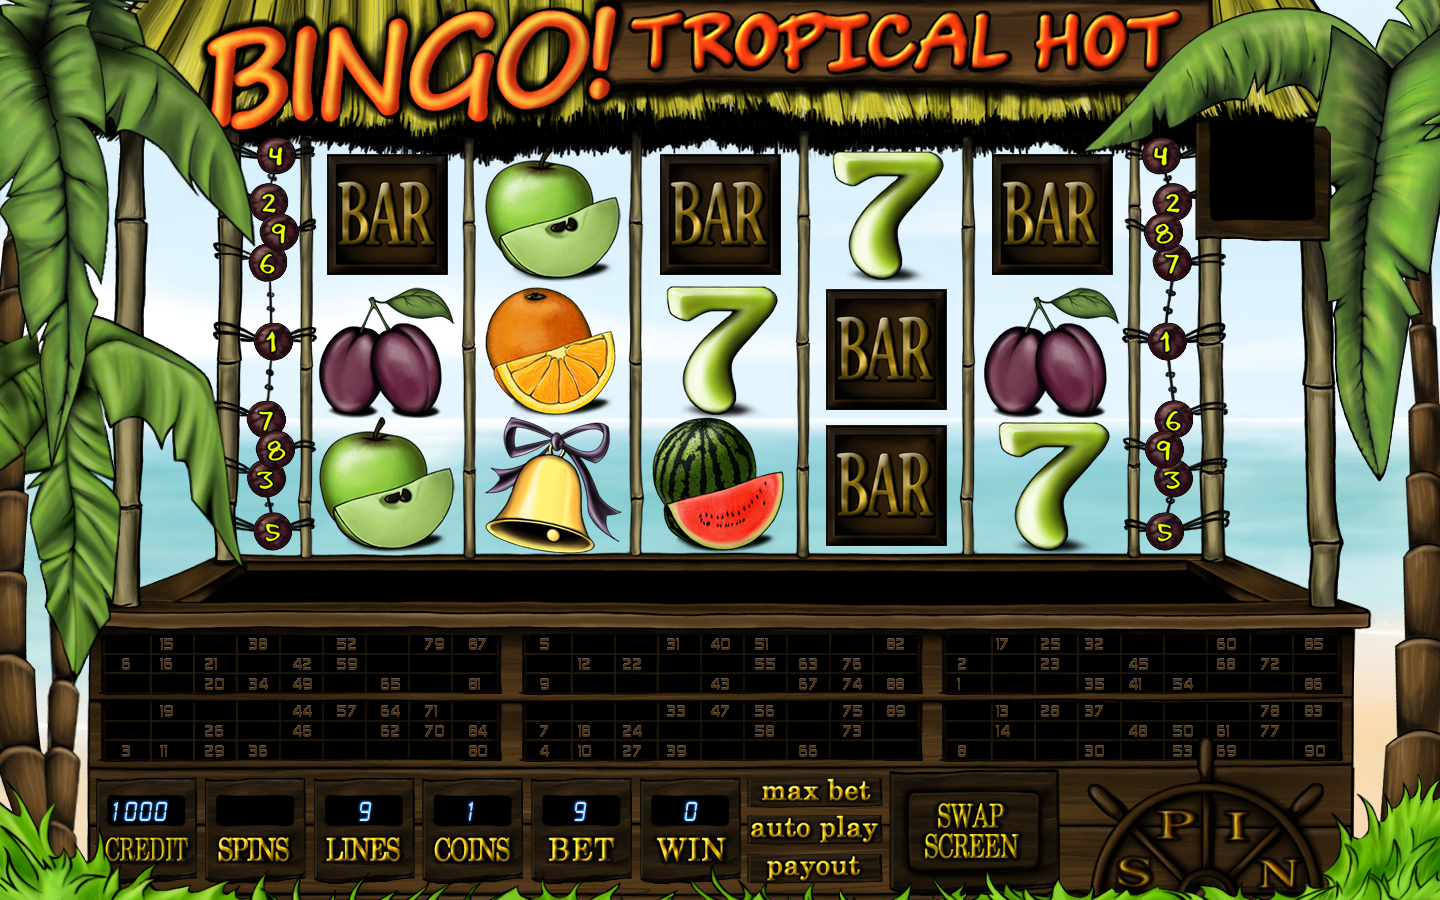
\includegraphics[width=\linewidth]{image002}
  \caption{Bingo Tropical Hot initial screen}
  \url{}
  \label{image002}
\end{figure}

The game consists of 5 reels and 3 visible rows (Figure \ref{image002}). It features 9 pay lines (Figure \ref{image028}). The total bet is calculated by multiplying the bet per line by the number of betting lines.

\begin{figure}[htbp]
  \centering
  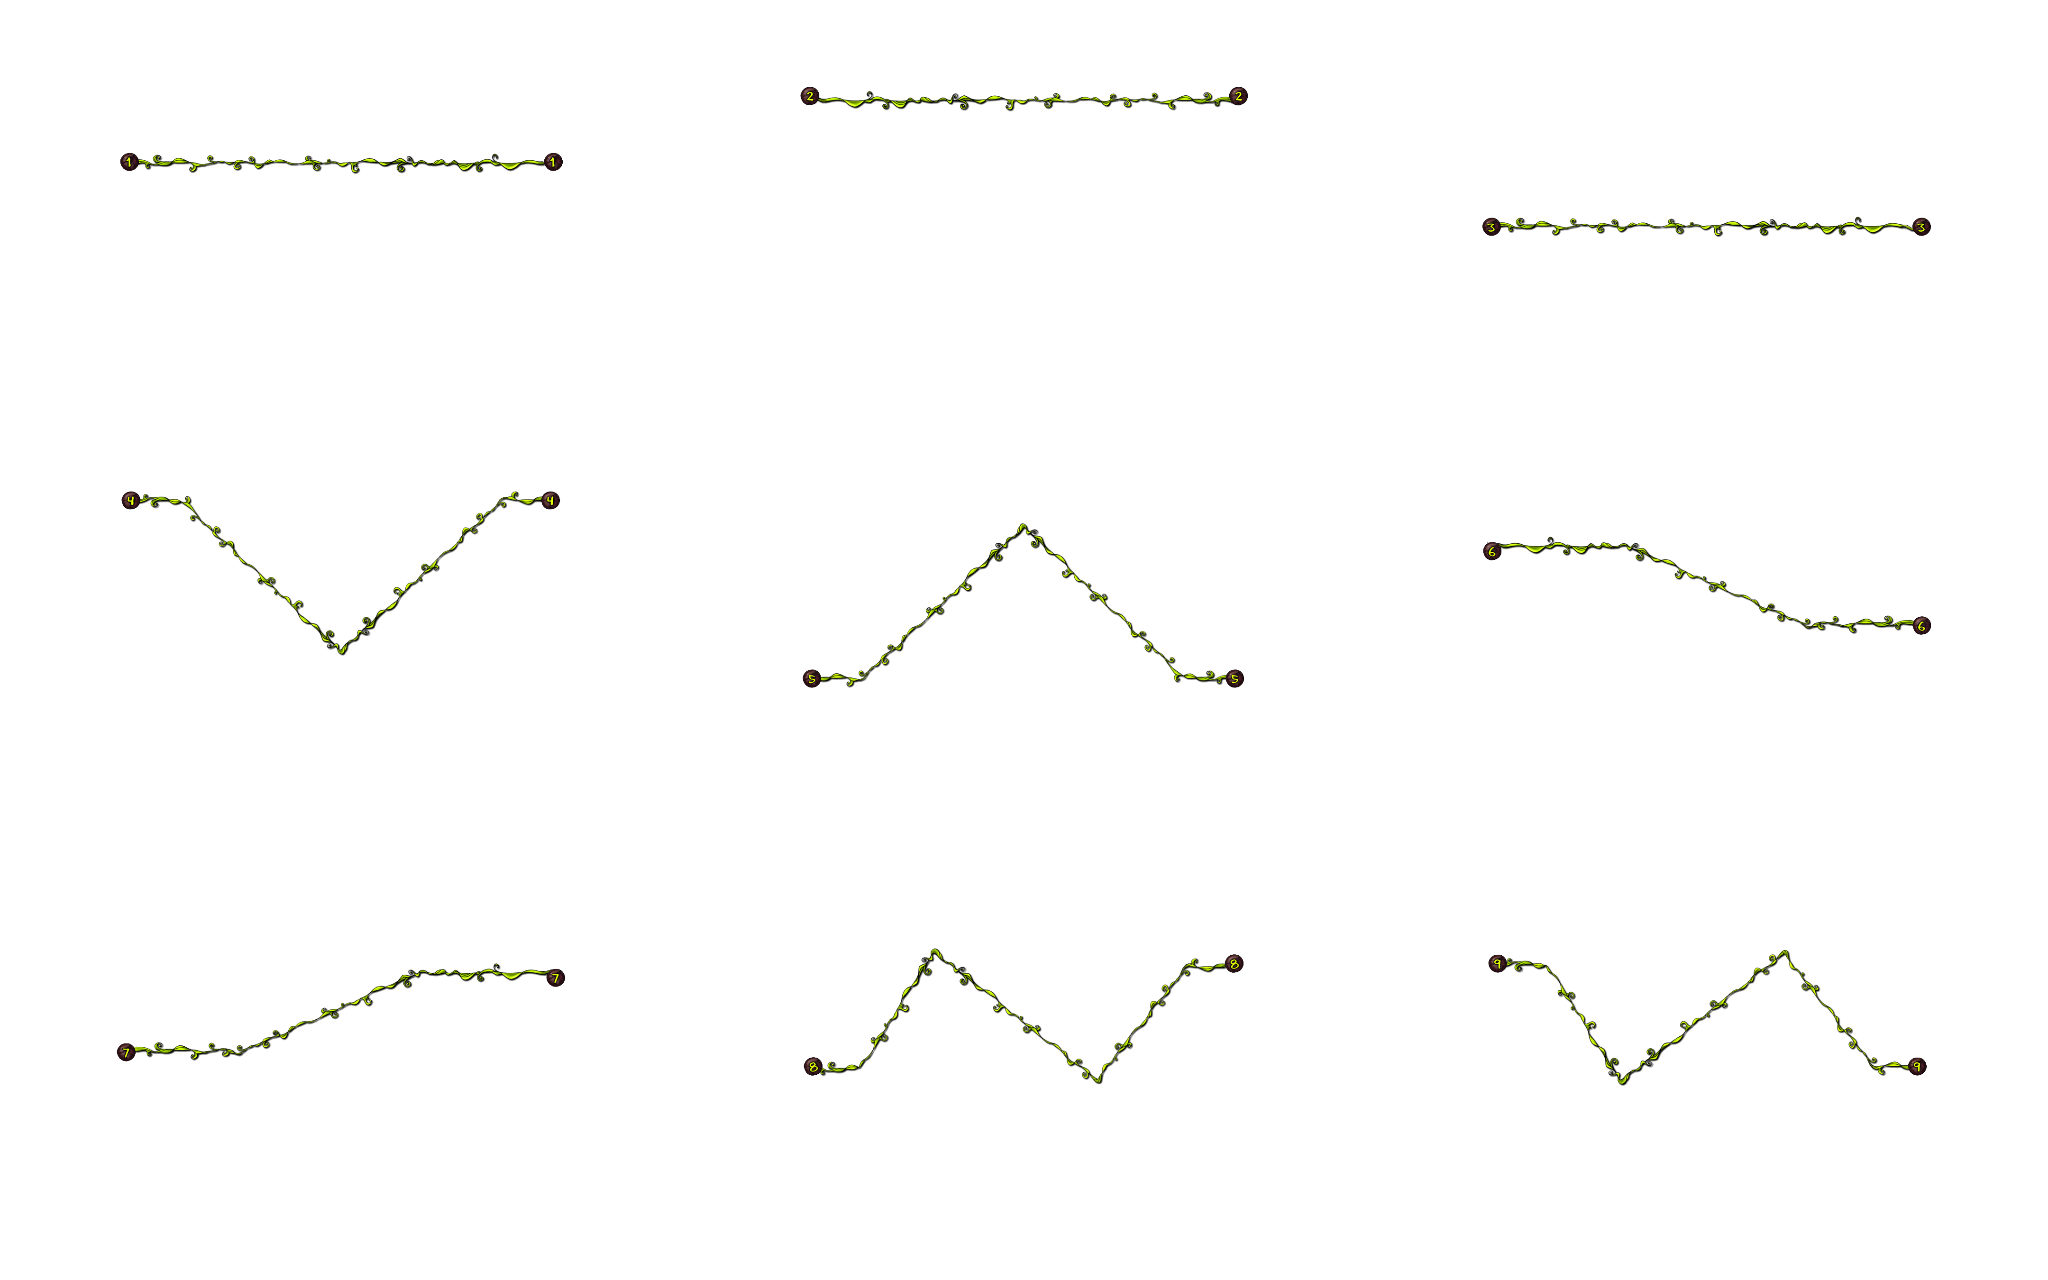
\includegraphics[width=\linewidth]{image028}
  \caption{Pay lines in Bingo Tropical Hot}
  \url{}
  \label{image028}
\end{figure}

All wins are counted from the leftmost reel to the rightmost. Wins are formed only on adjacent reels. There are 9 fixed paylines, and players cannot change the number of betting lines. All wins are multiplied by the bet per line, and only the highest win per line is paid out. The total bet for this game is the bet per line multiplied by 9.

\section*{Game Symbols}

\begin{figure}[htbp]
    \centering
    % === ROW 1 ===
    \begin{subfigure}[b]{0.18\textwidth}
        \centering
        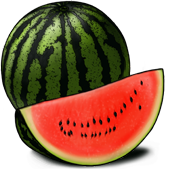
\includegraphics[width=\textwidth]{image004}
        \caption{}
    \end{subfigure}
    \hfill
    \begin{subfigure}[b]{0.18\textwidth}
        \centering
        
\includegraphics[width=\textwidth]{image005}
        \caption{}
    \end{subfigure}
    \hfill
    \begin{subfigure}[b]{0.18\textwidth}
        \centering
        
\includegraphics[width=\textwidth]{image006}
        \caption{}
    \end{subfigure}
    \hfill
    \begin{subfigure}[b]{0.18\textwidth}
        \centering
        
\includegraphics[width=\textwidth]{image007}
        \caption{}
    \end{subfigure}
    \hfill
    \begin{subfigure}[b]{0.18\textwidth}
        \centering
        
\includegraphics[width=\textwidth]{image008}
        \caption{}
    \end{subfigure}
 
    \vspace{1ex}

    % === ROW 2 ===
    \begin{subfigure}[b]{0.18\textwidth}
        \centering
        
\includegraphics[width=\textwidth]{image009}
        \caption{}
    \end{subfigure}
    \hfill
    \begin{subfigure}[b]{0.18\textwidth}
        \centering
        
\includegraphics[width=\textwidth]{image010}
        \caption{}
    \end{subfigure}
    \hfill
    \begin{subfigure}[b]{0.18\textwidth}
        \centering
        
\includegraphics[width=\textwidth]{image011}
        \caption{}
    \end{subfigure}
    \hfill
    \begin{subfigure}[b]{0.18\textwidth}
        \centering
        
\includegraphics[width=\textwidth]{image012}
        \caption{}
    \end{subfigure}
    \hfill
    \begin{subfigure}[b]{0.18\textwidth}
        \centering
        
\includegraphics[width=\textwidth]{image013}
        \caption{}
    \end{subfigure}

    \vspace{1ex}

    % === ROW 3 ===
    \begin{subfigure}[b]{0.18\textwidth}
        \centering
        
\includegraphics[width=\textwidth]{image014}
        \caption{}
    \end{subfigure}
    \hfill
    \begin{subfigure}[b]{0.18\textwidth}
        \centering
        
\includegraphics[width=\textwidth]{image015}
        \caption{}
    \end{subfigure}
    \hfill
    \begin{subfigure}[b]{0.18\textwidth}
        \centering
        
\includegraphics[width=\textwidth]{image016}
        \caption{}
    \end{subfigure}
    \hfill
    \hspace{0.18\textwidth}
    \hfill
    \hspace{0.18\textwidth}

    \caption{Symbols in Bingo Tropical Hot}
    \label{image004016}
\end{figure}

The game features 13 symbols (see Figure \ref{image004016}). When betting 1 coin per line, different regular symbols yield varying prizes. Developing the mathematical model will involve adjusting the rewards for wins based on the number of matching symbol combinations. This game includes a wild symbol, which can substitute for all other symbols except the scatter symbol. However, the wild symbol does not pay out if it is part of a winning combination. This design choice helps simplify the determination of winning combinations. High-paying symbols that appear in smaller quantities can outperform less-paying wilds when they are part of a winning combination with fewer symbols. A standard rule is that only the highest prize per line is awarded.

Regular symbols can form line-winning combinations, but the game also features a scatter symbol. Scatter wins occur when the scatter symbol appears anywhere on the screen, and these symbols do not need to be adjacent to each other. Only the highest number of scatter symbols will be rewarded with a prize. Scatter wins are independent of the single-line bet and are calculated based on the total bet amount. The payout for the scatter symbol is still subject to future modeling.

It is common for the scatter symbol to trigger a free spins feature, and the logic for these free spins will also be modeled in the future.

\section*{Free Spins and Bingo Bonus}

The game includes a free spins scatter symbol, which typically appears only on reels 2, 3, and 4. However, during the math modeling phase, this standard approach can be adjusted. The number of scatter symbols that land will determine how many free spins are activated. Additionally, the quantity of scatters can influence a multiplier for the wins during the free spins, such as x1, x2, or x3. It is also possible to restrict or limit retriggered free spins during this mode according to the base game rules. Free spins retriggering is another option to consider during game modeling.

\begin{figure}[htbp]
  \centering
  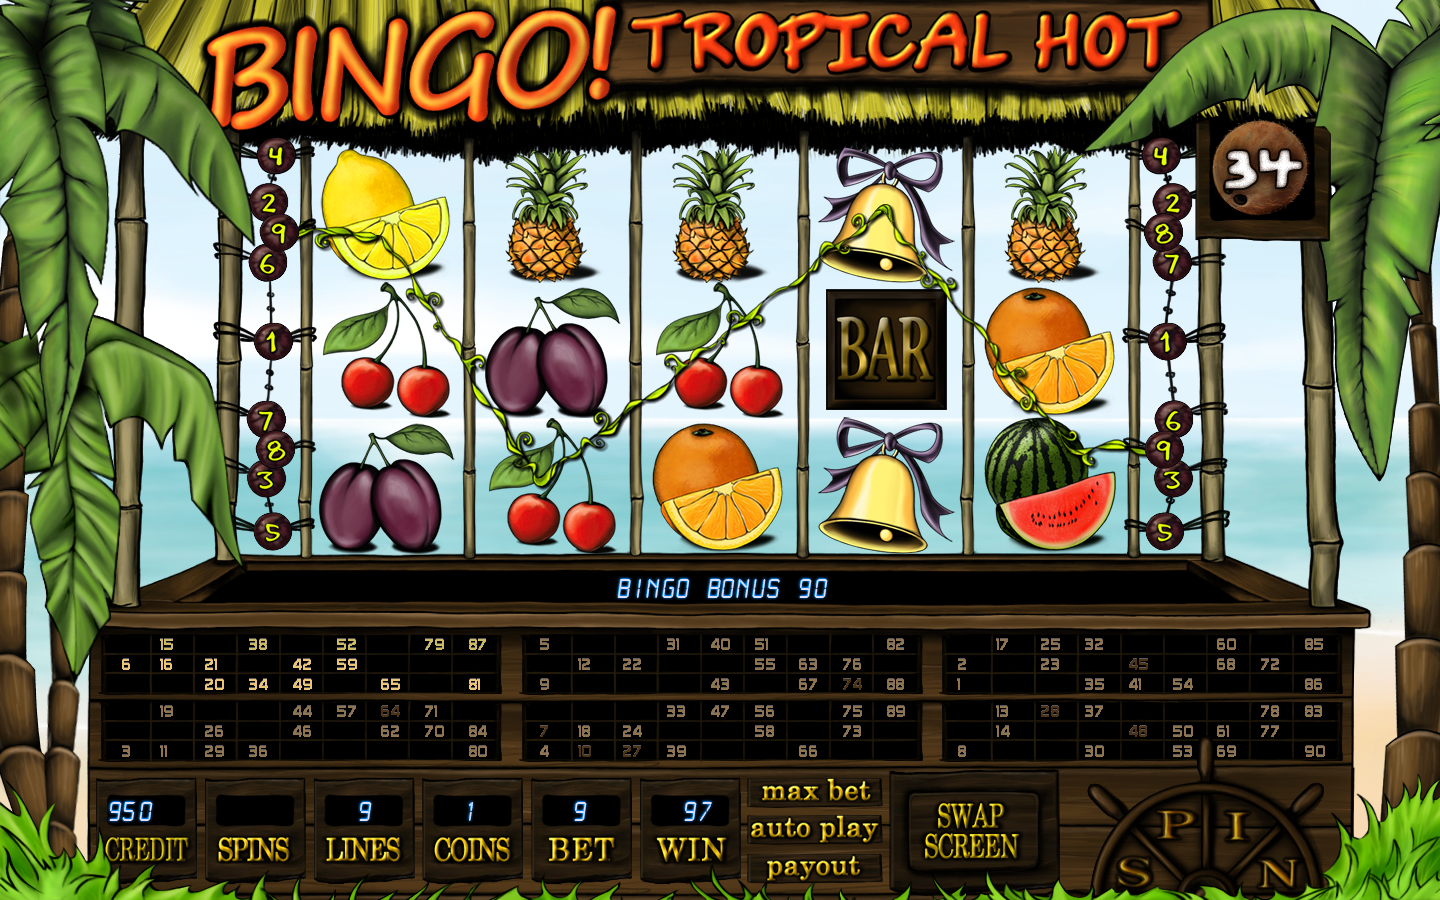
\includegraphics[width=\linewidth]{image003}
  \caption{Bonus screen of Bingo Tropical Hot}
  \url{}
  \label{image003}
\end{figure}

The game features a bingo bonus component at its core. At the bottom of the main screen, six bingo cards are displayed (Figure \ref{image003}). Bingo balls are drawn in the top right corner of the screen, using a standard set of bingo balls. Two types of bonuses are available - line combinations and bingo combinations. The amounts for both bonuses are determined through mathematical modeling. After a bingo bonus is awarded, the cards are reset. The bingo bonus in this slot machine game has a significant impact on the overall RTP, necessitating adjustments to all other prize amounts accordingly.

\chapter{PAR Sheet}

The mathematics behind slot machine games is typically outlined in a document known as a PAR Sheet. Most game studios create their PAR sheet as a Microsoft Excel file, but in current math modeling, a LibreOffice Calc file is used. This document includes all the key numbers and some aggregated statistics.

\section*{Game Summary}

The first section of the PAR sheet usually contains a general description of the game (Figure \ref{image025}).

\begin{figure}[htbp]
  \centering
  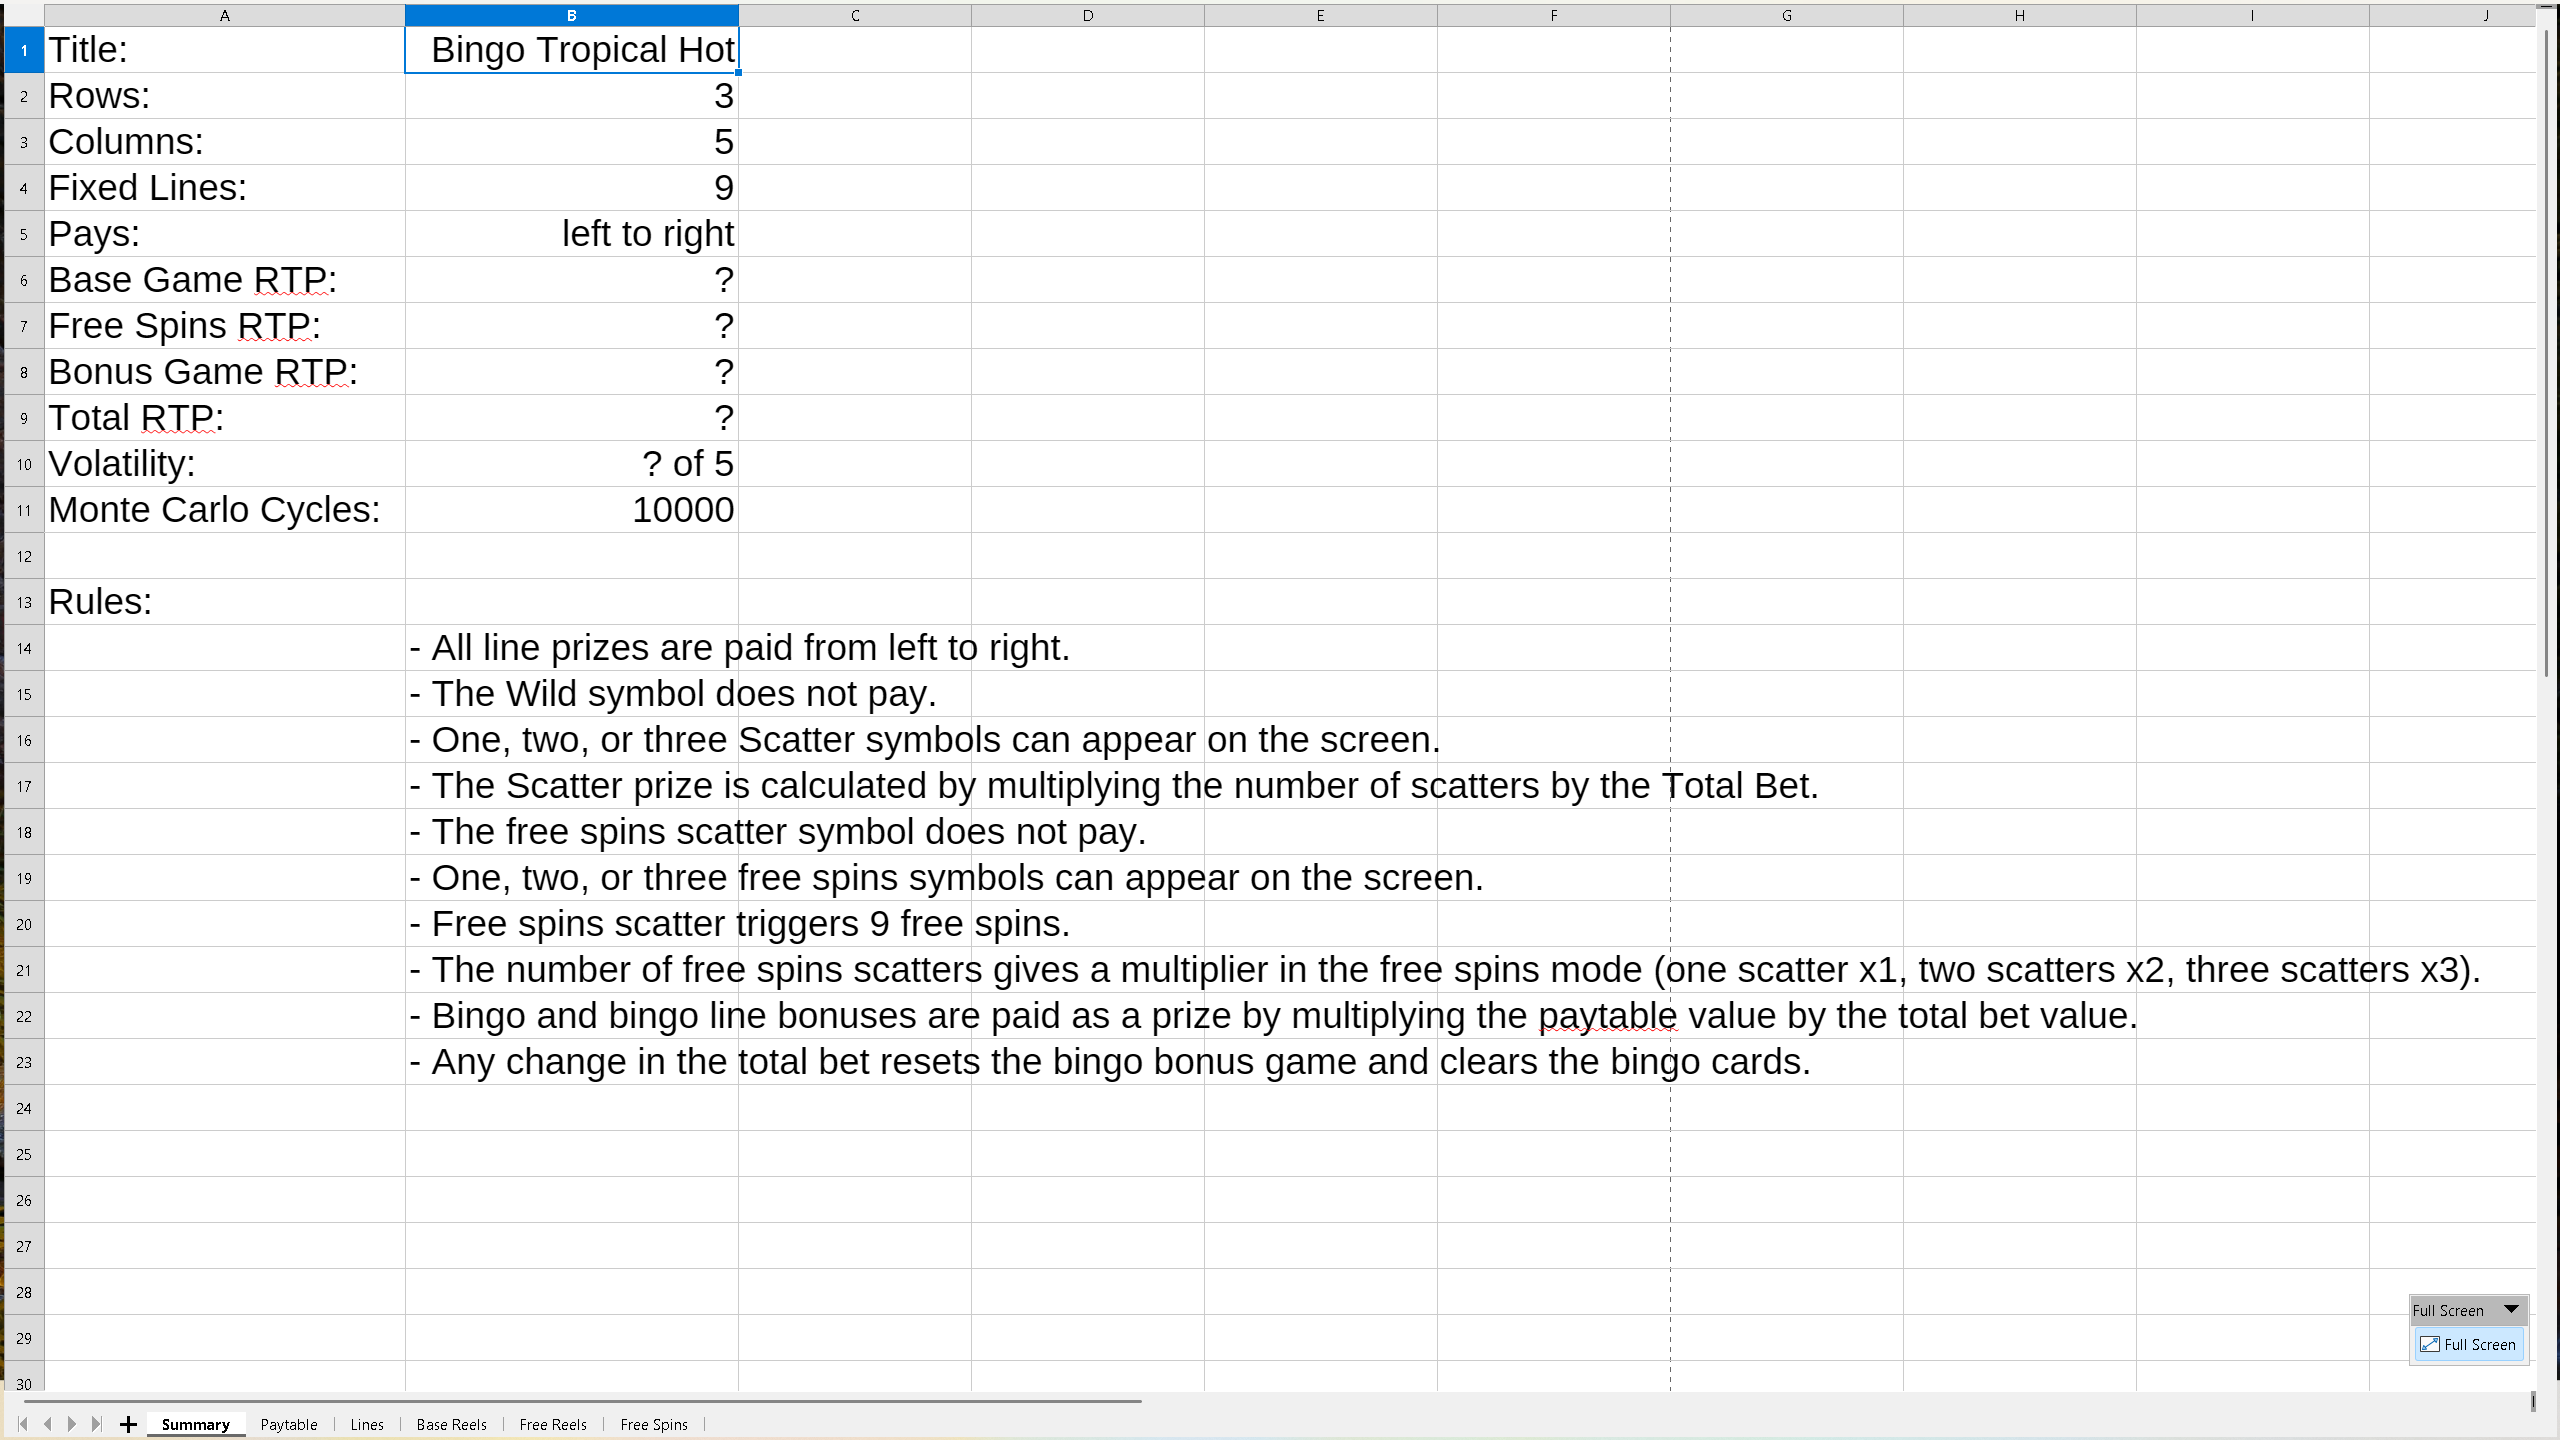
\includegraphics[width=\linewidth]{image025}
  \caption{Game summary}
  \url{}
  \label{image025}
\end{figure}

The game summary sheet gathers various information derived from values in other sheets.

\section*{Game Paytable}

The second sheet holds the list of symbols with the amount of reward each symbol can provide. This data structure is known as the paytable, and it forms the basis of the mathematical model. In some games, wild symbols can award a prize on their own, though this is not always the case. Most games typically include a scatter symbol that grants prizes regardless of its position within a winning combination on the screen (Figrure \ref{image026}).

\begin{figure}[htbp]
  \centering
  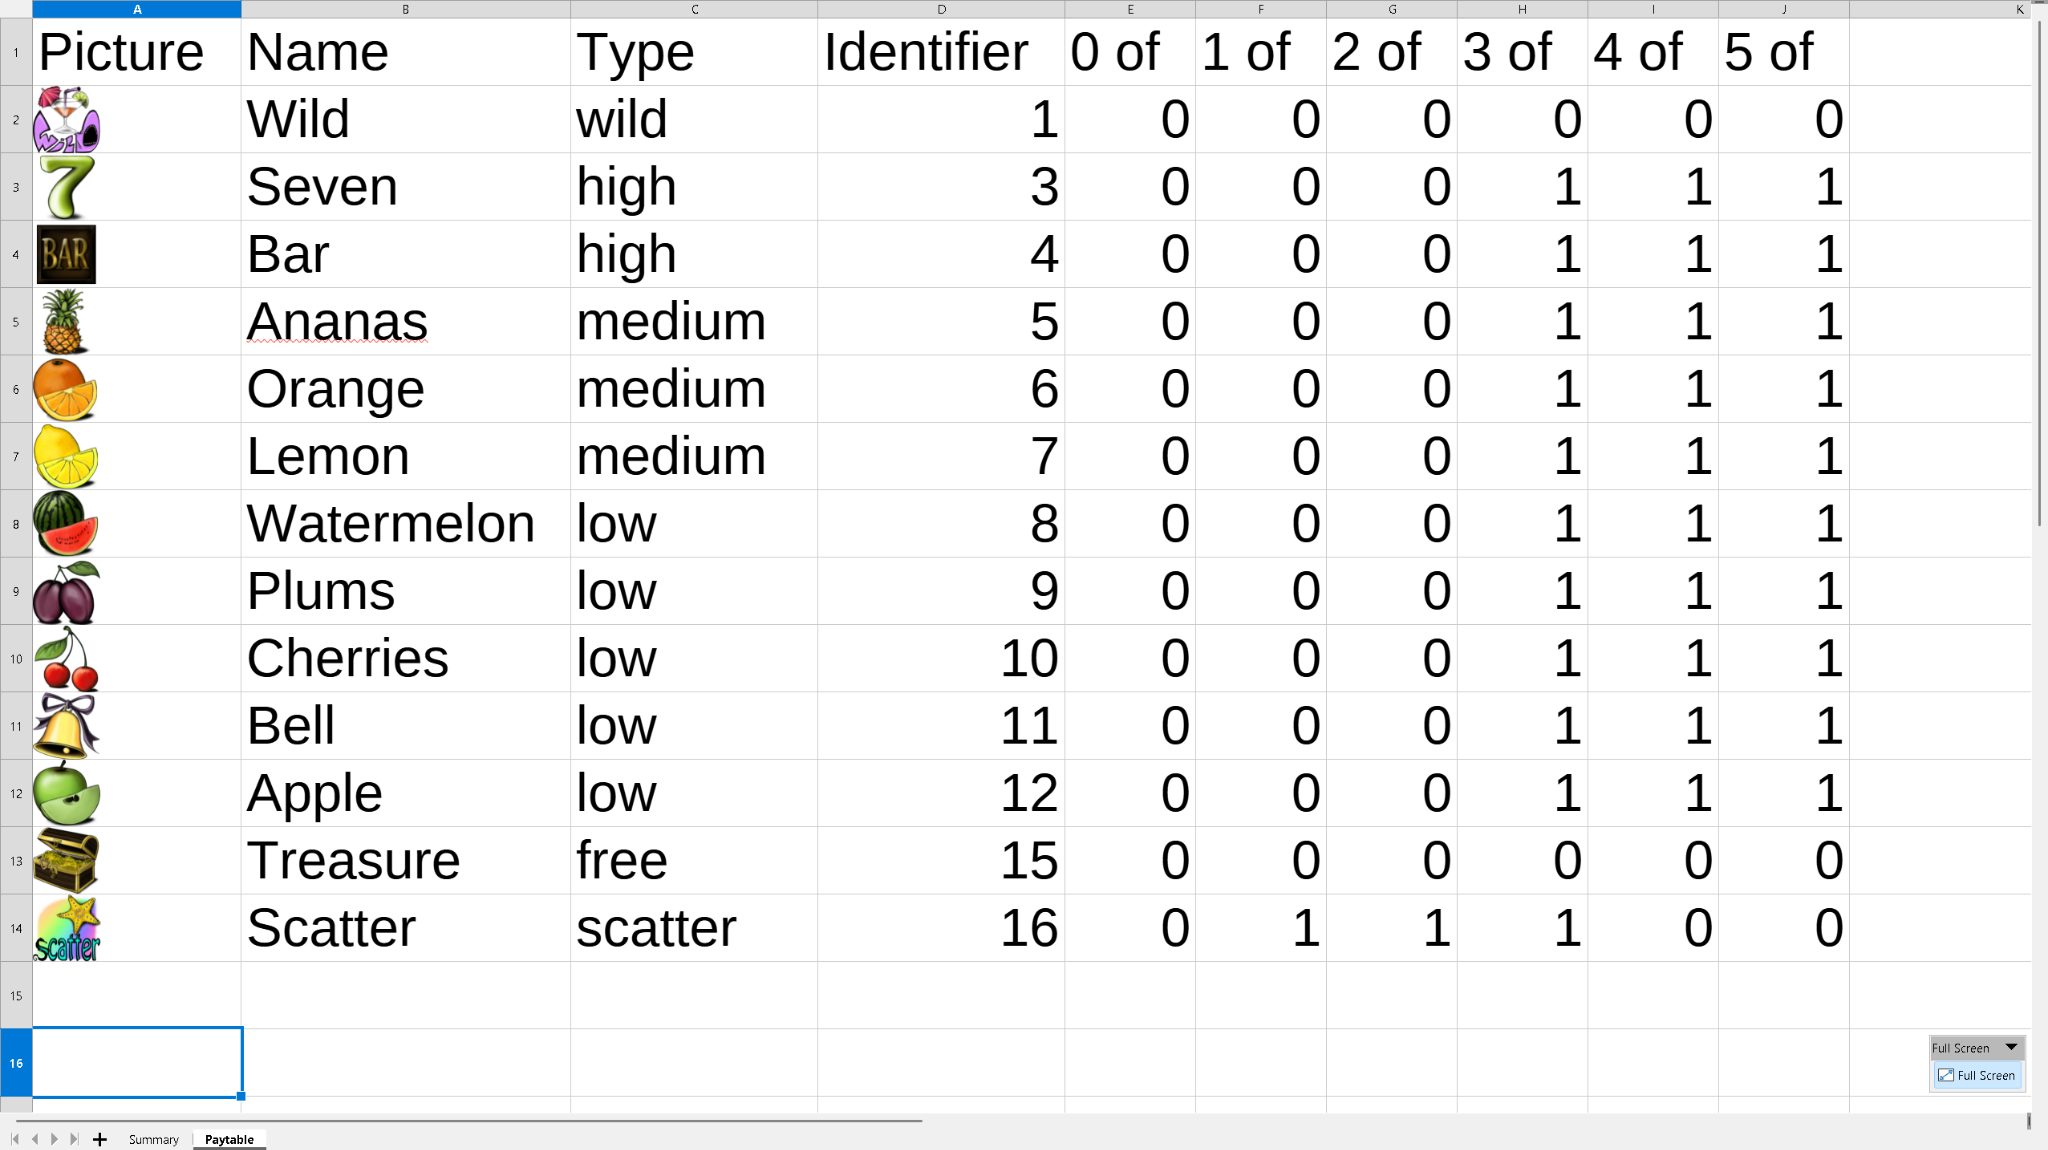
\includegraphics[width=\linewidth]{image026}
  \caption{The paytable of the game}
  \url{}
  \label{image026}
\end{figure}

Wins in this game are determined by the number of consecutive symbols that appear in a betting line combination. A high-paying symbol may award a win with just two symbols, but this will be confirmed in the future optimization of the mathematical model. It is important to note that the wild symbol does not provide a payout on its own. By omitting payouts for wild symbols, we can avoid confusion regarding which combinations are the most profitable on a single line.

The scatter symbol does pay out, but the free spins symbol does not yield a win by itself. There are a total of nine fixed betting lines, and when a bet of one coin is placed on a single line, the total bet for each base game round amounts to nine coins. Prize rewards for regular symbols are displayed in the paytable based on a single bet of one coin per line. In contrast, scatter wins are calculated based on the total bet.

Initially, all prize values in the Paytable are set to one for mathematical modeling. These values will be adjusted later during the optimization process. Specific game parameters, including the number of symbols, the number of betting lines, free spin symbols, and scatter symbols, are determined by the art and game designers. Most of these parameters are not subject to mathematical optimization, as they are focused more on aesthetics and gaming experience.

\section*{Game Lines}

The primary method for winning prizes on slot machines is through line combinations, where symbols must typically align from left to right. The number of betting lines can vary, ranging from a single line to all possible combinations. In some cases, lines may also be calculated from right to left, or even in both vertical directions - top to bottom and vice versa. Additionally, certain games employ cluster mechanics instead of traditional betting lines. For example, in Bingo Tropical Hot, there are only nine lines that are counted from left to right (Figure \ref{image027}).

\begin{figure}[htbp]
  \centering
  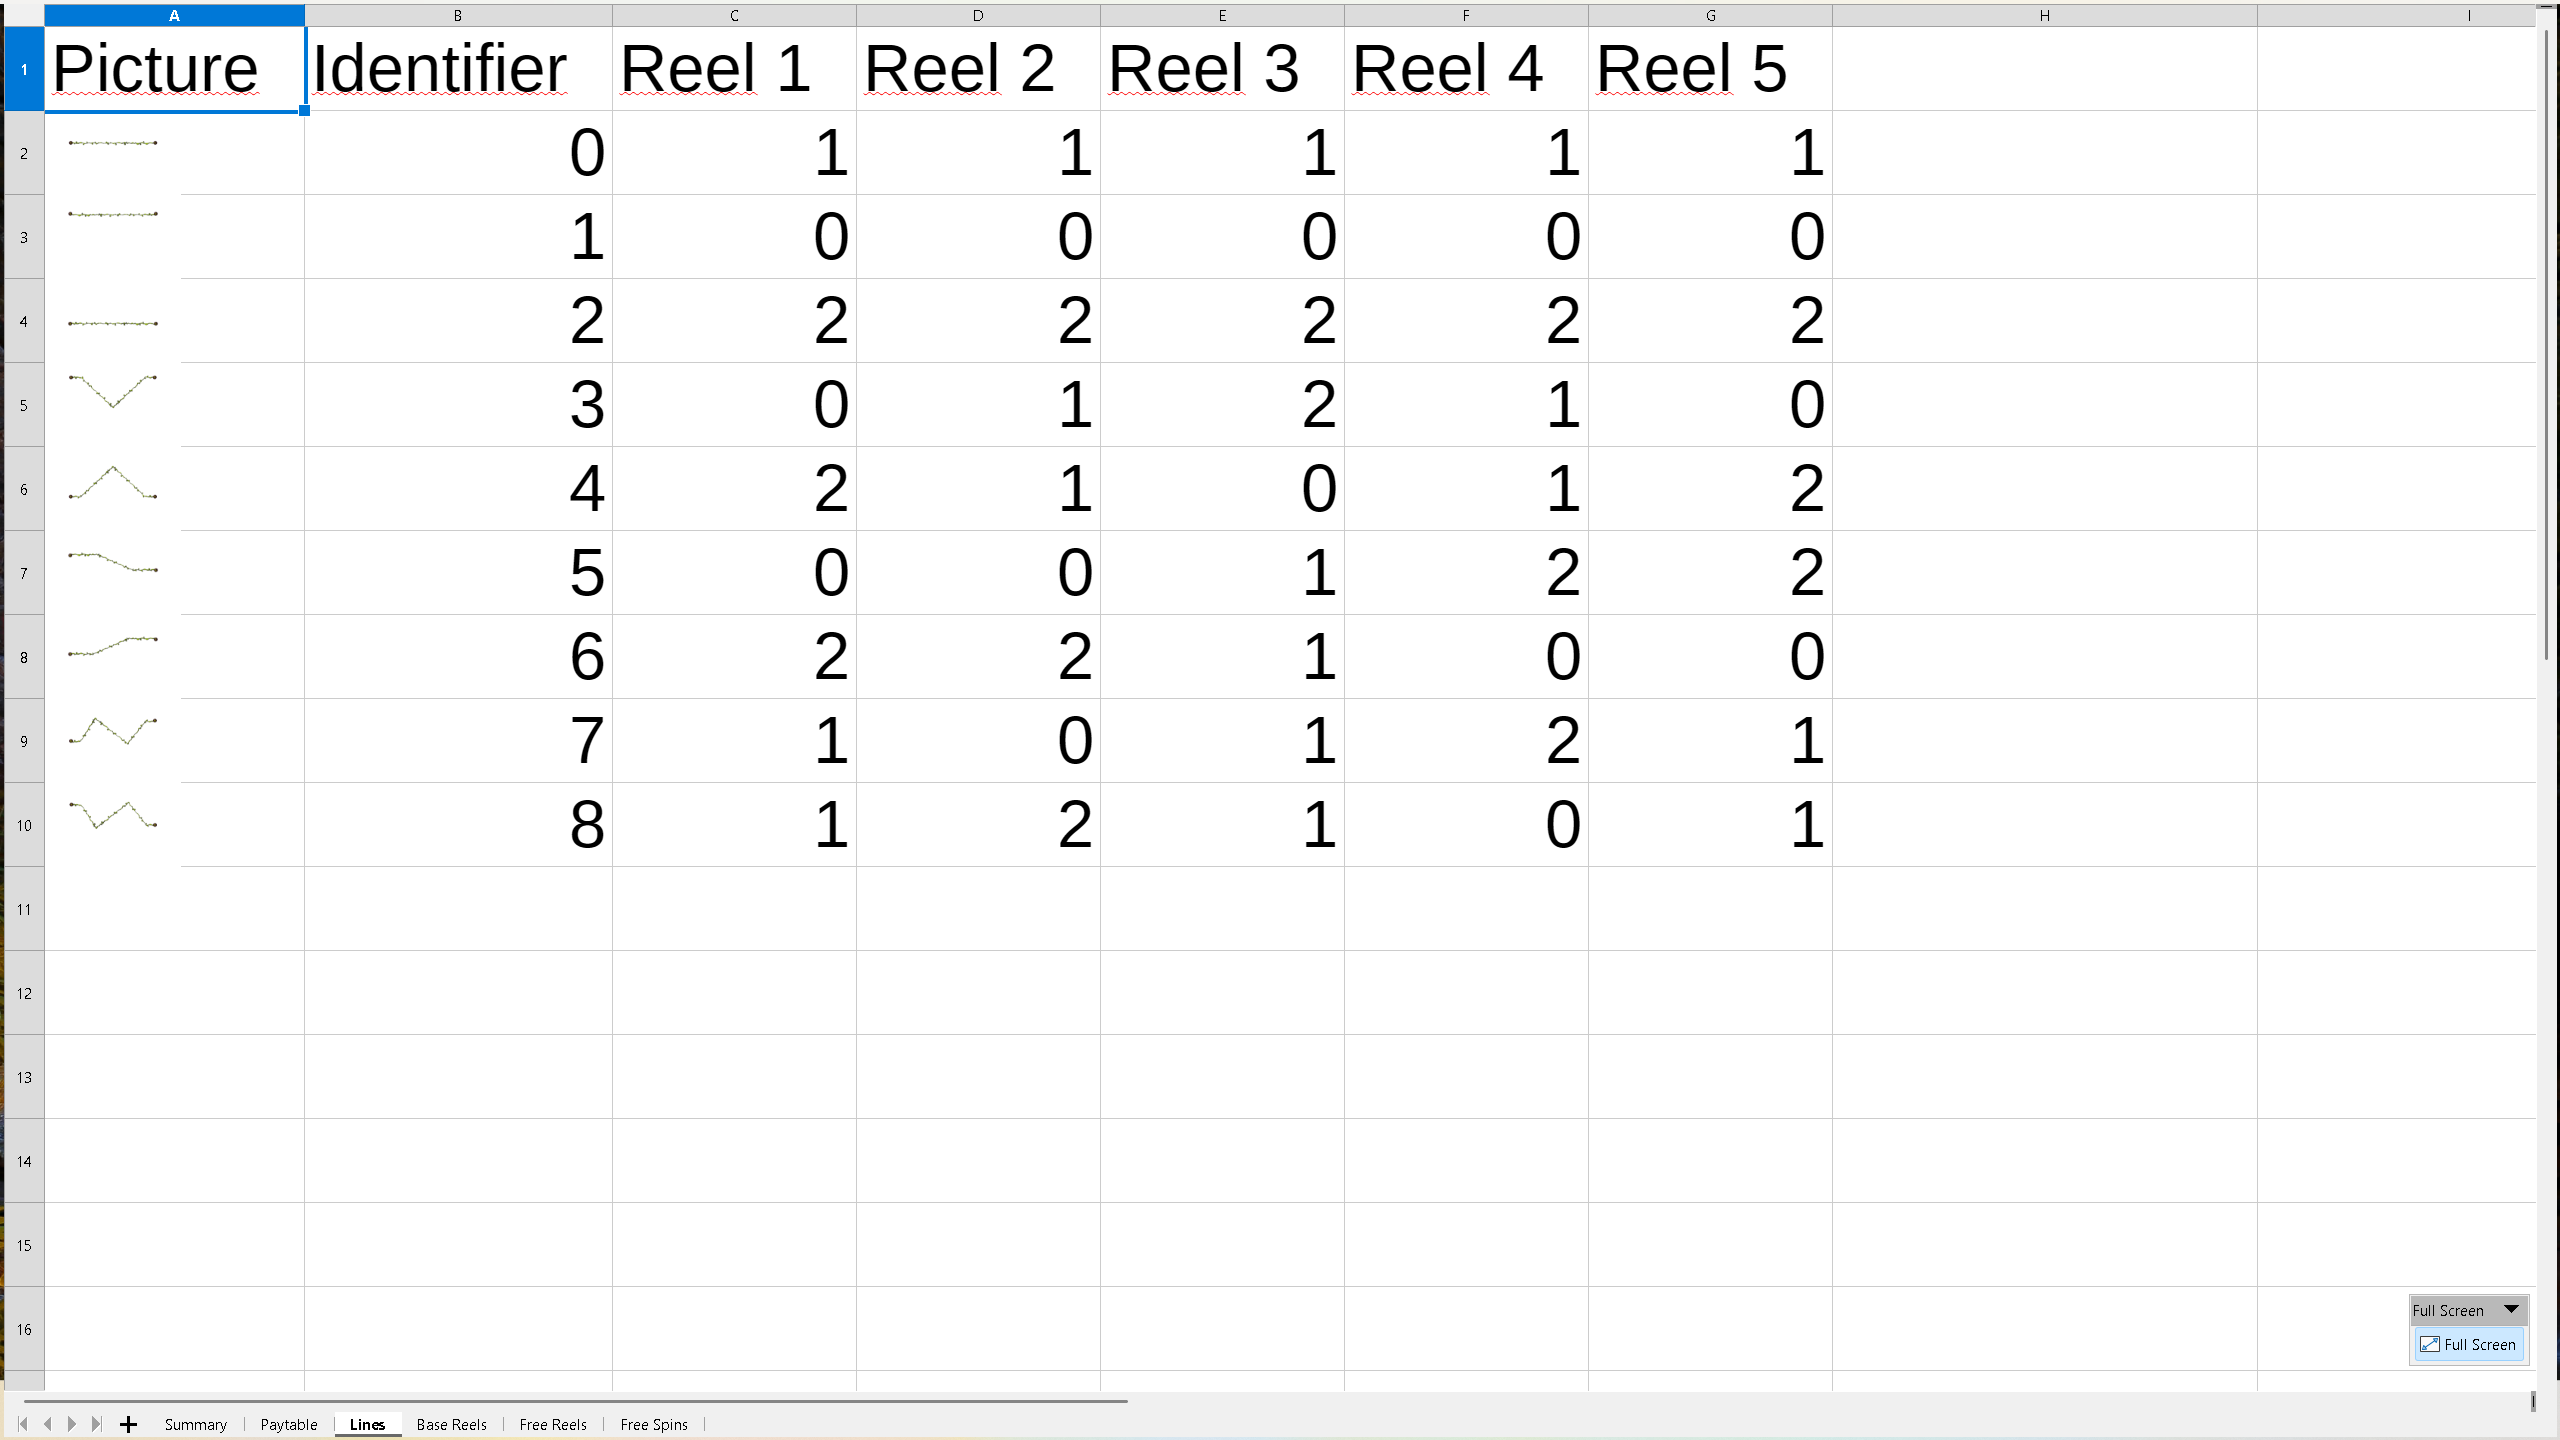
\includegraphics[width=\linewidth]{image027}
  \caption{The betting lines in the game}
  \url{}
  \label{image027}
\end{figure}

Each position in the betting lines sheet indicates the offset from the top of the screen for each reel. This representation simplifies the implementation of win calculations for the different betting lines by programmers.

\section*{Base Game and Free Spins Reels}

There are various approaches to presenting game reels, with the most common being based on traditional mechanical games. This method represents virtual reels as a sequence of numbers that indicate the placement of symbols on each reel. In some rare cases, reels may be represented using a weighted table or in other analytical forms. The discrete probabilistic model of the reels is the most straightforward method for approval of the RTP.

The length of the reels and the specific positions of the symbols are determined through mathematical optimization and game design choices. The final mathematical model must comply with all legal regulatory requirements and align with the financial profit expectations of the gambling game operator. Ultimately, it should also satisfy the players, as they are the ones investing their money into the game.

\begin{figure}[htbp]
  \centering
  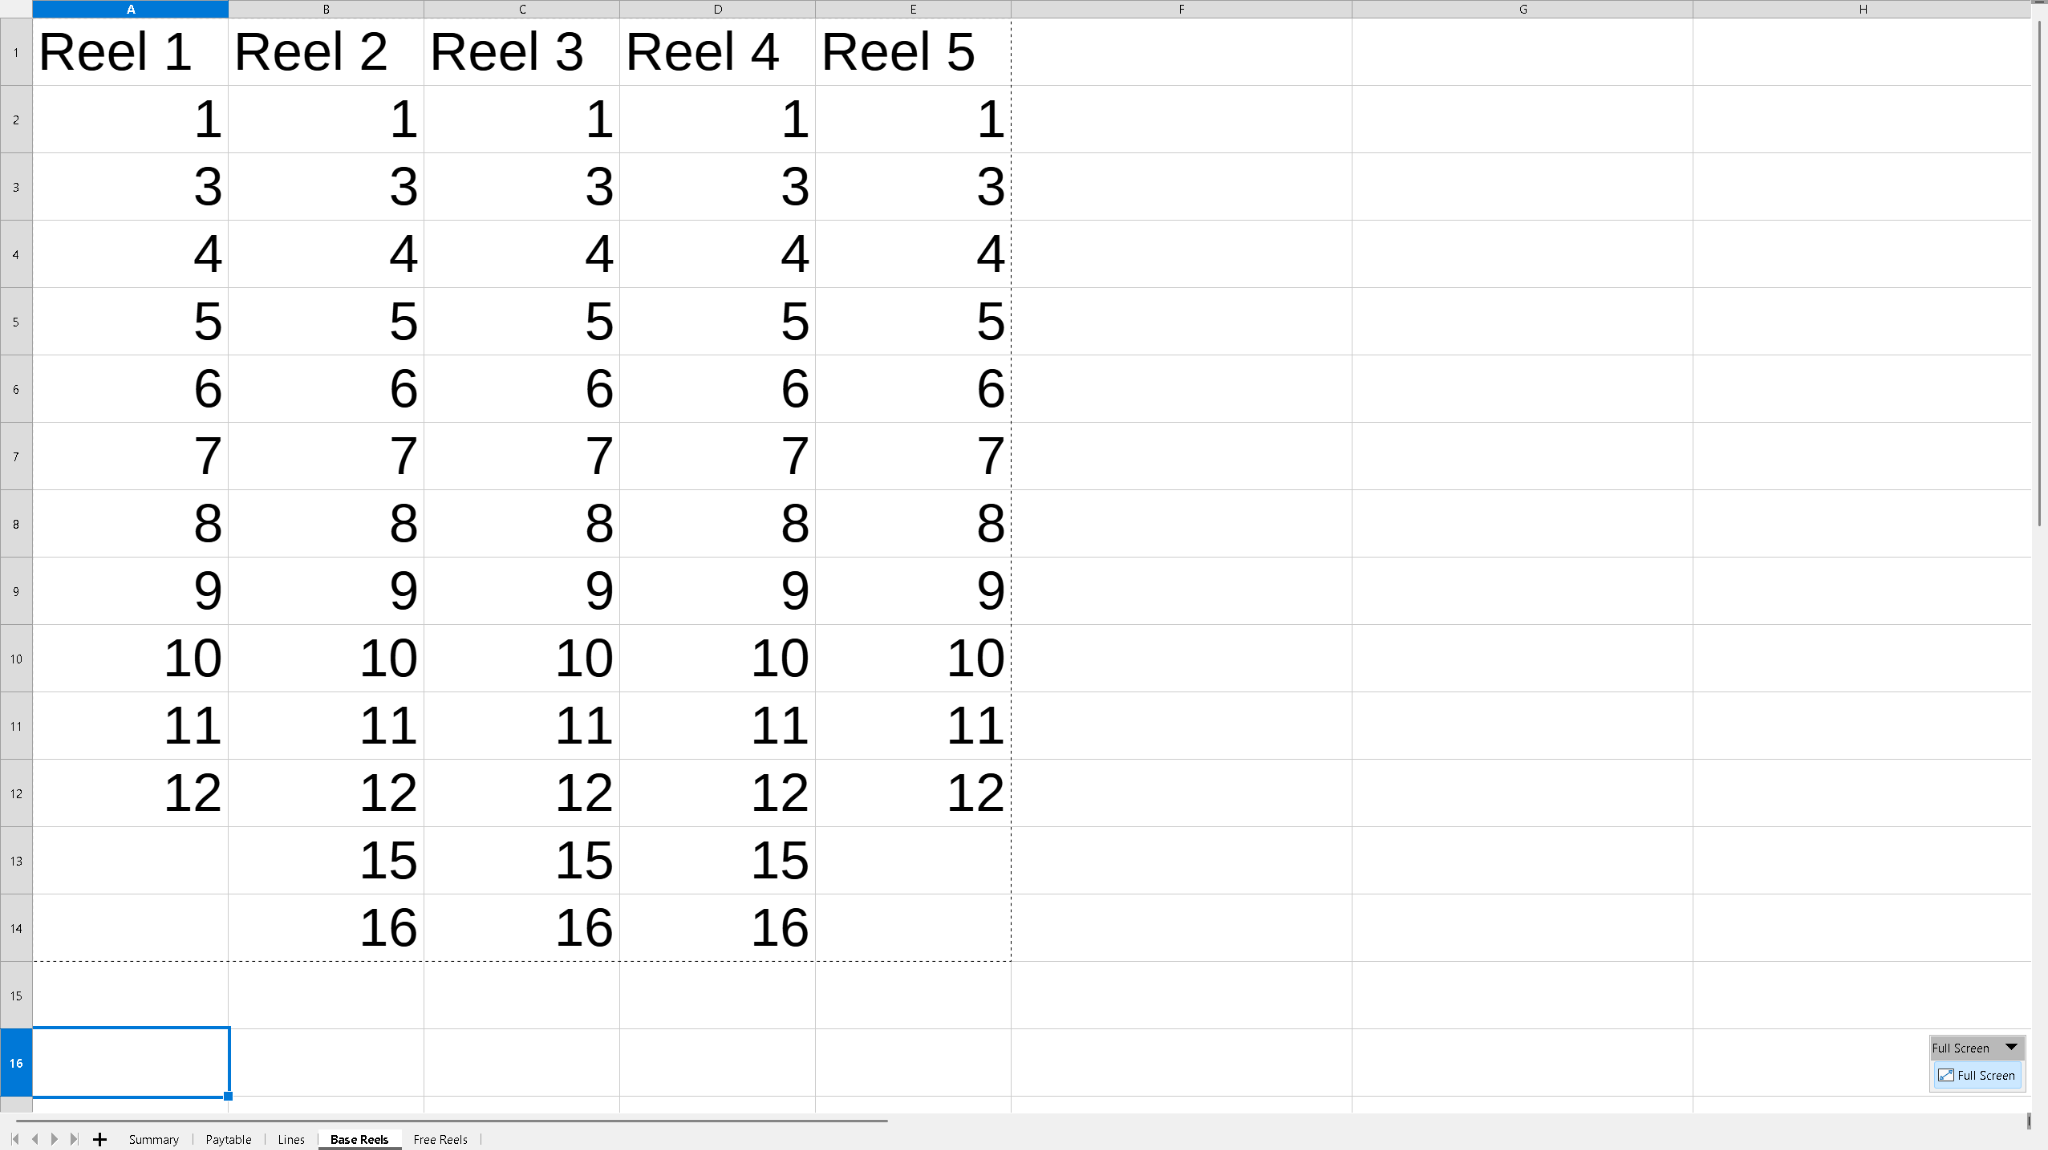
\includegraphics[width=\linewidth]{image023}
  \caption{Base game reels}
  \url{}
  \label{image023}
\end{figure}

In the base game and during free spins, the reel sets typically differ. This difference is due to the expectation that free spins will be more profitable for the player. In some instances, multiple reel sets can be utilized for both the base game and free spins.

For the current optimization of the math model, a single set of reels is used for the base game. Initially, each symbol appears only once on each reel, and the symbols are arranged in consecutive order. The scatter symbols and those that trigger free spins are restricted to the middle reels only (Figure \ref{image023}).

\begin{figure}[htbp]
  \centering
  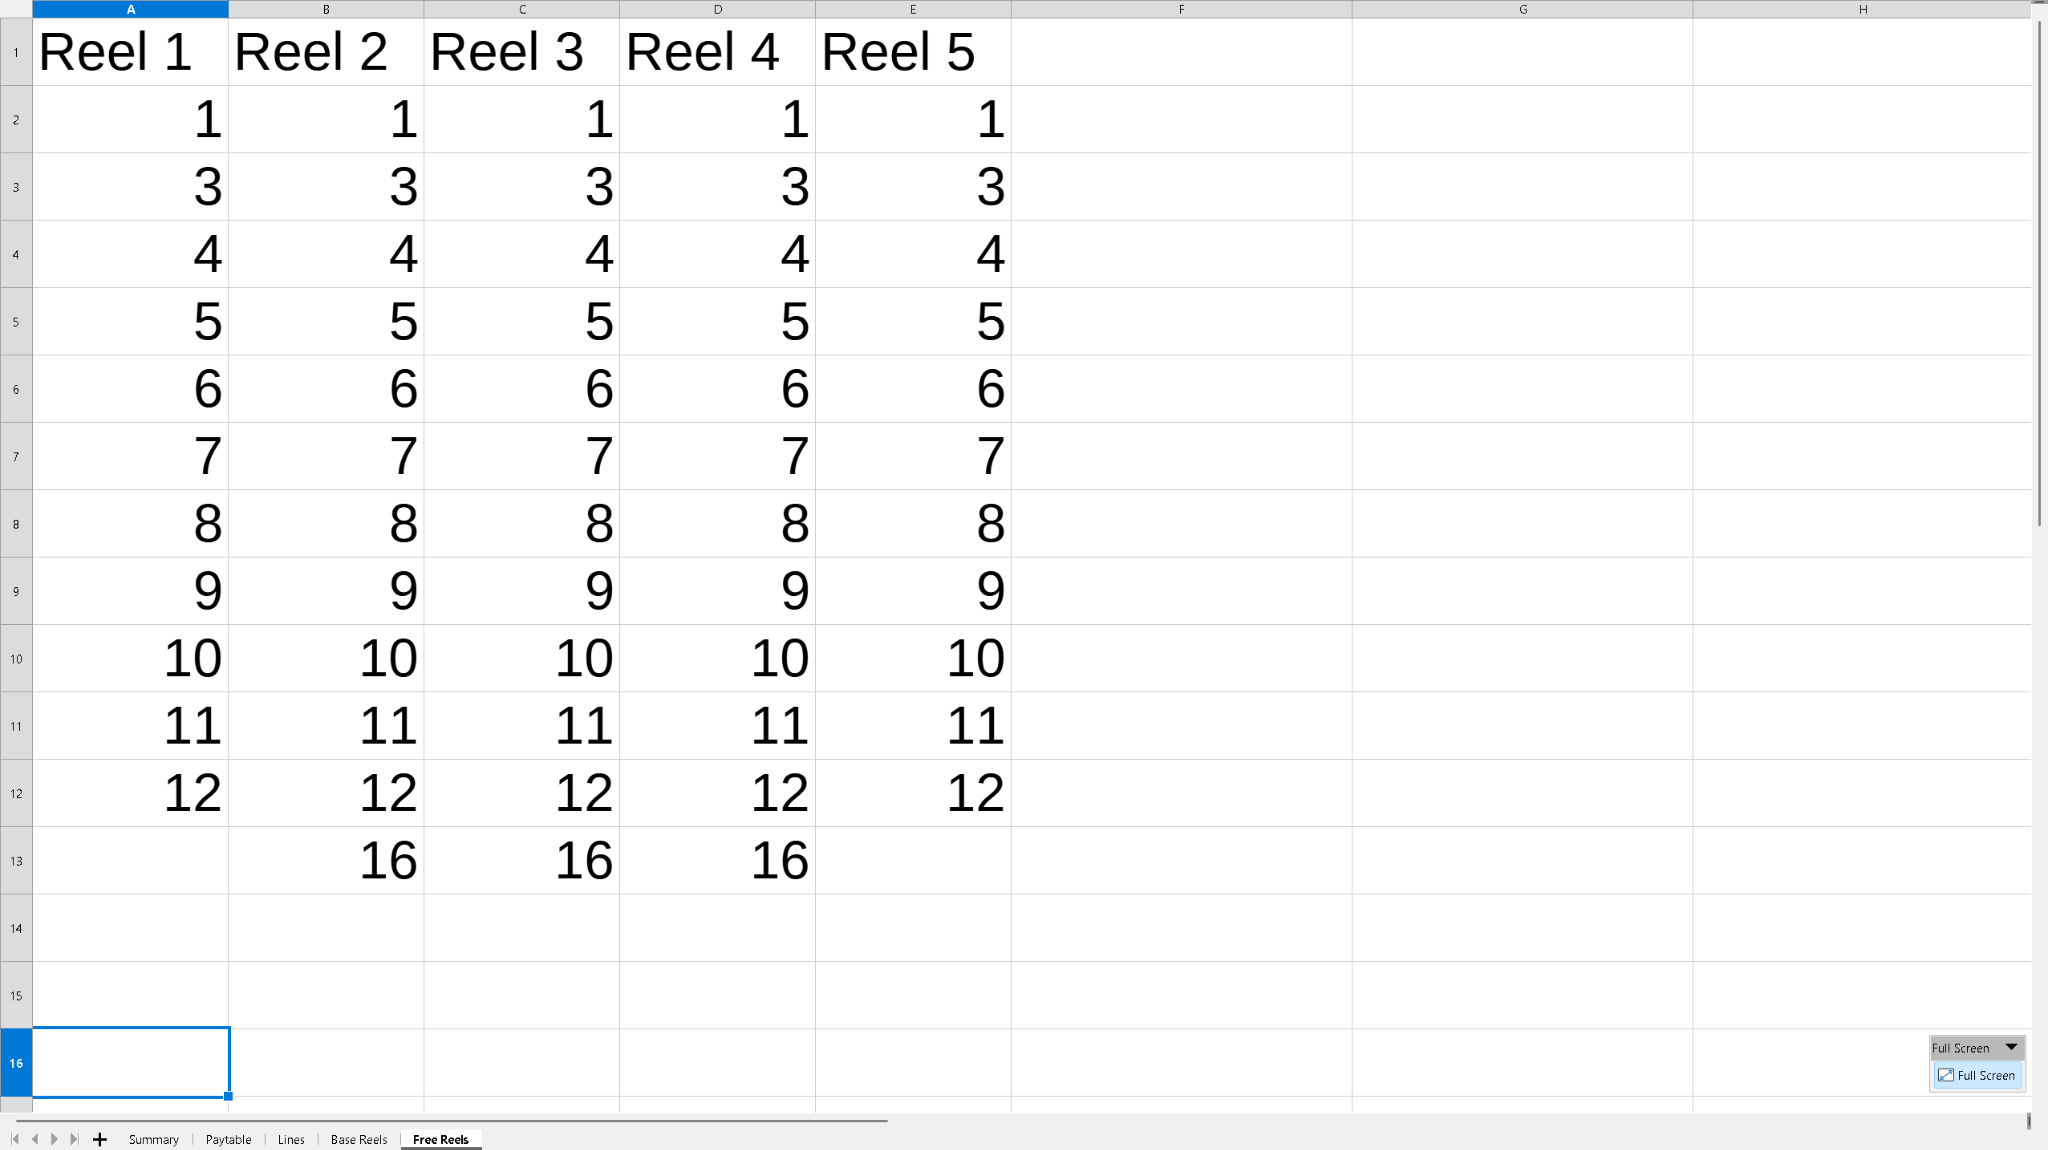
\includegraphics[width=\linewidth]{image024}
  \caption{Free spins reels}
  \url{}
  \label{image024}
\end{figure}

The only change in the initial free spins reels is the removal of the symbol that triggers free spins (Figure \ref{image024}). At this stage of game model optimization, retriggering free spins is not possible.

\chapter{Programming Language Selection}

The gambling industry has widely adopted Microsoft Excel as the standard tool for the mathematical design of slot machine games. While Excel is a powerful resource for creating PAR sheets, LibreOffice Calc can be used even more effectively and is more cost-effective. Calc is compatible with major operating systems such as Windows, macOS, and various Linux distributions. Additionally, Calc offers superior support for programming languages compared to Excel.

The mathematical modeling process for Bingo Tropical Hot will heavily rely on Monte Carlo simulations. Therefore, it’s essential that the simulation source code be closely aligned with Calc's data structures.

\section*{Possible Programming Languages}

LibreOffice Calc supports several scripting languages through its UNO (Universal Network Objects) API. The primary scripting languages available are StarBasic, Python, JavaScript, BeanShell, Java, and other UNO-compatible languages. StarBasic is the most integrated language in LibreOffice and resembles VBA, although it is not entirely compatible with it.

Modern versions of LibreOffice support Python natively, allowing for interaction with LibreOffice Calc through its UNO API. Python scripts can be stored internally within LibreOffice documents. Additionally, LibreOffice supports JavaScript through a Rhino-based variant via the Script Provider, which operates within LibreOffice’s JVM-based scripting framework. BeanShell, a lightweight Java-like scripting language, is also supported through LibreOffice’s Java-based scripting framework.

Java serves as the most advanced programming language for writing macros and extensions in LibreOffice. Since the UNO API is language-independent, scripting can also be performed using C++, .NET, or other languages via the UNO bridge, but these methods are typically used for external programs rather than for embedded macros.

The selection of a programming language is a common consideration in software development projects. Several criteria are used to evaluate languages, with performance, the richness of software libraries, available documentation, and robustness often being the most important factors.

For current mathematical modeling, Java is the preferred choice. Its performance generally surpasses that of most scripting languages. Java utilizes both a compiler and a JVM to interpret its class files. Additionally, the strong integration with LibreOffice is a significant advantage. LibreOffice originated from OpenOffice, which was initially created by Sun Microsystems - the same company that developed the Java programming language. Even in modern versions of LibreOffice, many modules are still written in Java.

Another critical factor in selecting a programming language is the competence of the development team. For instance, if Java and Python have similar scores based on the other criteria, the language that the team is more familiar with should be chosen.

\chapter{Setup of Simulation Project}

To model the slot math, start by installing the LibreOffice software, which is available for the most popular operating systems. Next, install the Java development tools, such as openJDK or Oracle JDK. Finally, configure Java (Figure \ref{image022}) in LibreOffice by navigating to Tools -> Options -> LibreOffice -> Advanced.

\begin{figure}[htbp]
  \centering
  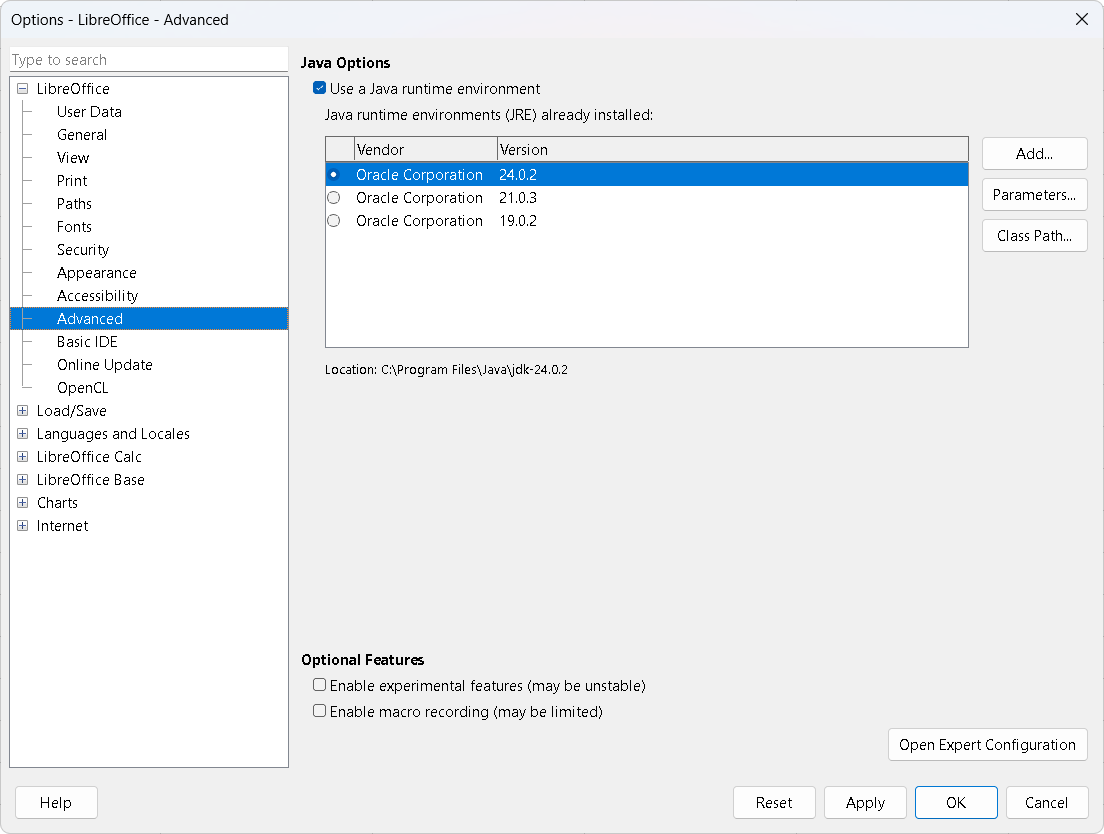
\includegraphics[width=\linewidth]{image022}
  \caption{Java configuration in LibreOffice}
  \url{}
  \label{image022}
\end{figure}

Slot games are based on combinatorial math models. There are various approaches to designing and simulating these games. A slot game can be developed entirely without a computer, using only a pencil and paper. Most elements of a slot game can be fine-tuned by calculating theoretical parameters. This book adopts a practical approach, recreating the game model through empirical adjustments and Monte Carlo simulations ( \url{https://en.wikipedia.org/wiki/Monte_Carlo_method} ).

\section*{Source Code Repository}

The software project of the simulation is publicly available on GitHub:

\url{https://github.com/TodorBalabanov/Secrets-of-Slot-Machine-Mathematics-Development-Revealed}

\section*{Setting-up Gradle Project}

To create a Java plugin for LibreOffice, first establish a proper directory structure for the source code. The recommended structure is as follows (Listing \ref{listing001}).

\begin{lstlisting}[language=bash, caption={Project structure}, label=listing001]
simulator/
   build.gradle
   settings.gradle
   parcel-descriptor.xml
   src/
      main/
         java/
            eu/
               veldsoft/
                  bths/
                     Simulator.java
\end{lstlisting}

In this structure, the files `build.gradle` and `settings.gradle` define the parameters for building the project. The `parcel-descriptor.xml` file contains important information for integrating the Java plugin with LibreOffice. The initial source code for the game simulator will be placed in the `Simulator.java` file.

The Gradle build system settings are specified in the `settings.gradle` file, which for the current project only includes the project name (Listing \ref{listing002}).

\begin{lstlisting}[language=bash, caption={settings.gradle}, label=listing002]
	rootProject.name = 'Bingo-Tropical-Hot-Simulator'
\end{lstlisting}

All important project configuration options are specified in the `build.gradle` file (Listing \ref{listing003}). The version of the JAR file will be 1.0.0, and this version will be reflected in the name of the JAR file. It is considered a best practice for each Java software solution to reside in its own package. For this development project, the package will be `eu.veldsoft.bths`. Within the Gradle script, the exact locations of the LibreOffice directories are defined to ensure that the compiled plugin can be deployed appropriately. The deployment process involves copying the Java archive and the descriptor file into the appropriate LibreOffice directory structure.

\begin{lstlisting}[language=bash, caption={build.gradle}, label=listing003]
plugins {
    id 'java'
}

group = 'eu.veldsoft.bths'
version = '1.0.0'

/**
 * Detect LibreOffice classes folder on different OSes
 */
def detectLibreOfficeClassesDir() {
    def candidates = []

    if (System.properties['os.name'].toLowerCase().contains('win')) {
        candidates <<
        "${System.getenv('ProgramFiles')}\\LibreOffice\\program\\classes"
        candidates <<
        "${System.getenv('ProgramFiles(x86)')}\\LibreOffice\\program\\classes"
    } else if (System.properties['os.name'].toLowerCase().contains('mac')) {
        candidates <<
        "/Applications/LibreOffice.app/Contents/Resources/java"
    } else {
        // Assume Linux/Unix-like
        candidates << "/usr/lib/libreoffice/program/classes"
        candidates << "/usr/share/libreoffice/program/classes"
    }

    return candidates.find { new File(it, "libreoffice.jar").exists() }
}

def libreOfficeClassesDir = detectLibreOfficeClassesDir()

if (libreOfficeClassesDir == null) {
    throw new GradleException(
	"Could not find libreoffice.jar -
	please install LibreOffice or set LIBREOFFICE_HOME.")
}

repositories {
    flatDir {
        dirs libreOfficeClassesDir
    }
}

dependencies {
    implementation name: 'libreoffice'
}

java {
    sourceCompatibility = JavaVersion.VERSION_1_8
    targetCompatibility = JavaVersion.VERSION_1_8
}

jar {
    archiveBaseName = 'Bingo-Tropical-Hot-Simulator'
    from sourceSets.main.output
    manifest {
        attributes(
            'Main-Class': 'eu.veldsoft.bths.Simulator'
        )
    }
}

tasks.register('deploy', Copy) {
    dependsOn jar
    from("${buildDir}/libs/${jar.archiveFileName.get()}")
    from("parcel-descriptor.xml")

    def loUserScripts = System.getProperty('os.name').toLowerCase().
    contains('win') ?
        "${System.getenv('APPDATA')}\\LibreOffice\\4\\user\\
        Scripts\\java\\Bingo-Tropical-Hot-Simulator" :
        "${System.getProperty('user.home')}/.config/libreoffice/4/user/
        Scripts/java/Bingo-Tropical-Hot-Simulator"

    into(loUserScripts)
}
\end{lstlisting}

Each JAR plugin must be accompanied by a descriptor file named `parcel-descriptor.xml` (Listing \ref{listing004}). This descriptor defines the programming language used, provides the name and description of the plugin, and specifies the entry point function. Additionally, it contains crucial information about the JAR file that houses the plugin itself.

\begin{lstlisting}[language=xml, caption={parcel-descriptor.xml}, label=listing004]
<?xml version="1.0" encoding="UTF-8"?>
<parcel language="Java" xmlns:parcel="scripting.dtd">
  <script language="Java">
    <locale lang="en">
      <displayname value="Bingo Tropical Hot Simulator" />
      <description>
      Run simulation of Bingo Tropical Hot slot machine.
      </description>
    </locale>
    <functionname value="eu.veldsoft.bths.Simulator.simulate"/>
    <logicalname value="eu.veldsoft.bths.Simulator.simulate"/>
    <languagedepprops>
      <prop name="classpath" value="Bingo-Tropical-Hot-Simulator-1.0.0.jar"/>
    </languagedepprops>
  </script>
</parcel>
\end{lstlisting}

The macro source code will be provided within a class named `eu.veldsoft.bths.Simulator`.

After creating the directory, a Gradle wrapper should be generated by using the following command (Listing \ref{listing005}).

\begin{lstlisting}[language=bash, caption={Wrapper generation}, label=listing005]
gradle wrapper
\end{lstlisting}

The `gradlew` command is a small script included in Gradle-based projects, which allows anyone to run Gradle without needing to install it system-wide.

To build the JAR file, use this command (Listing \ref{listing006}).

\begin{lstlisting}[language=bash, caption={JAR file building}, label=listing006]
gradlew clean build
\end{lstlisting}

To deploy the created plugin, use the following command (Listing \ref{listing007}).

\begin{lstlisting}[language=bash, caption={Plug-in deployment}, label=listing007]
gradlew deploy
\end{lstlisting}

The commands can be executed in a sequence (Listing \ref{listing008}).

\begin{lstlisting}[language=bash, caption={Chain execution}, label=listing008]
clear && gradlew clean build deploy
\end{lstlisting}

After the deployment process, the JAR file along with the descriptive file will be available in the LibreOffice Java plugins directory, making the plugin ready for use.

\begin{figure}[htbp]
  \centering
  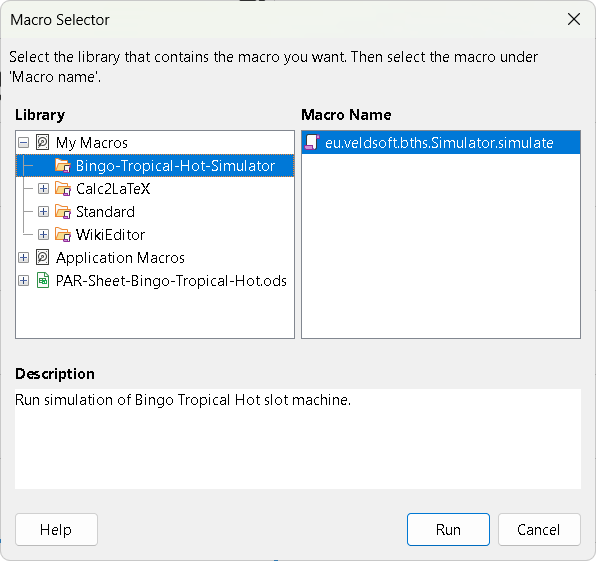
\includegraphics[width=\linewidth]{image017}
  \caption{Running the macro}
  \url{}
  \label{image017}
\end{figure}

Access the newly created plugin from the Tools -> Macros -> Run Macro... menu (Figure \ref{image017}).

\chapter{Common Data Structures}

Software development consists of two main components - data structures and algorithms. These elements are closely interconnected - good data modeling results in efficient and high-performing algorithms. In many software development processes, data structure modeling is completed before implementing algorithms (Listing \ref{listing009}). This same approach will be followed in this writing.

\begin{lstlisting}[language=Java, caption={Macro single entry point}, label=listing009]
package eu.veldsoft.bths;

import com.sun.star.script.provider.XScriptContext;

public class Simulator {
    public static void simulate(XScriptContext ctx) {
    }
}
\end{lstlisting}

To ensure that the development tools are set up correctly and that the building process is accurate, a good approach is to write simple source code in the style of a "Hello World" program. The easiest way to start is by entering some text into cell A1 (Listing \ref{listing010}).

\begin{lstlisting}[language=Java, caption={Writing text in a cell}, label=listing010]
package eu.veldsoft.bths;

import com.sun.star.script.provider.XScriptContext;
import com.sun.star.uno.UnoRuntime;
import com.sun.star.frame.XModel;
import com.sun.star.sheet.XSpreadsheetDocument;
import com.sun.star.container.XIndexAccess;
import com.sun.star.sheet.XSpreadsheet;

public class Simulator {
    public static void simulate(XScriptContext ctx) {
        try {
            XModel model = ctx.getDocument();
            XSpreadsheetDocument document =
            UnoRuntime.queryInterface(XSpreadsheetDocument.class, model);
            XIndexAccess sheets =
            UnoRuntime.queryInterface(XIndexAccess.class, document.getSheets());
            XSpreadsheet first =
            UnoRuntime.queryInterface(XSpreadsheet.class, sheets.getByIndex(0));


            first.getCellByPosition(0, 0).setFormula("Simulation!");
        } catch (Exception e) {
            e.printStackTrace();
        }
    }
}
\end{lstlisting}

Many popular software products utilize a plugin-based architecture, and LibreOffice is among them. This product features a comprehensive internal document object model. One significant advantage of plugin-based software solutions is that they allow access to this internal document object model through various scripting languages.

In the case of the Java plugin, it accesses the active document via the XModel object. A reference to the document itself is provided as an XSpreadsheetDocument object. From this document object, users can access the LibreCalc sheets. Once the first sheet is selected, text can be written in the cell identified by the logical address A1.

\section*{Source of Entropy}

As previously mentioned, modern computerized gambling games depend significantly on a reliable source of entropy. There are several options available, but when it comes to the Java programming language, the two primary choices are the Random class and the SecureRandom class. The SecureRandom class has the advantage of providing cryptographically secure numbers, but it comes at a cost of its performance, which is generally slower compared to the Random class (Listing \ref{listing011}).

\begin{lstlisting}[language=Java, caption={RNG class import}, label=listing011]
package eu.veldsoft.bths;

import java.security.SecureRandom;

import com.sun.star.script.provider.XScriptContext;
import com.sun.star.uno.UnoRuntime;
import com.sun.star.frame.XModel;
import com.sun.star.sheet.XSpreadsheetDocument;
import com.sun.star.container.XIndexAccess;
import com.sun.star.sheet.XSpreadsheet;

public class Simulator {
        private static final SecureRandom PRNG = new SecureRandom();
     
    public static void simulate(XScriptContext ctx) {
        try {
            XModel model = ctx.getDocument();
            XSpreadsheetDocument document =
            UnoRuntime.queryInterface(XSpreadsheetDocument.class, model);
            XIndexAccess sheets =
            UnoRuntime.queryInterface(XIndexAccess.class, document.getSheets());
            XSpreadsheet first =
            UnoRuntime.queryInterface(XSpreadsheet.class, sheets.getByIndex(0));

            first.getCellByPosition(0, 0).setFormula("Simulation!");
        } catch (Exception e) {
            e.printStackTrace();
        }
    }
}
\end{lstlisting}

The instance of the RNG is private, as it will only be used within the simulation class. The field is marked as final because the RNG instance will be created only once. It is also static, ensuring that each method in the class uses the same single instance of the RNG.

\section*{Paytable}

The game paytable is a fundamental element in each slot machine. It shows the payout for each winning combination. Most of the case wins are calculated from left to right. When reels are five, usually wins are formed by 3, 4, or 5 consecutive symbols. The Bingo Tropical Hot paytable can be represented as a two-dimensional array (Listing \ref{listing012}). The first dimension gives the number of consequent symbols. In contrast, the second shows the index of a particular symbol. Each cell in the array provides the prize amount.

\begin{lstlisting}[language=Java, caption={Paytable array model}, label=listing012]
private static int paytable[][] = {};

XSpreadsheet paytable = UnoRuntime.queryInterface(XSpreadsheet.class,
sheets.getByName("Paytable"));
int tableRows = 0;
int tableColumns = 0;
for (int c = 4; paytable.getCellByPosition(c,1).getType()!=
CellContentType.EMPTY; c++) {
	tableColumns++;
}
for (int r = 1; paytable.getCellByPosition(4, r).getType()!=
CellContentType.EMPTY; r++) {
	tableRows++;
}
Simulator.paytable = new int[tableRows][tableColumns];
for (int c = 0; c<tableColumns; c++) {
	for (int r = 0; r<tableRows; r++) {
		Simulator.paytable[r][c] = (int)paytable.getCellByPosition(4+c,
		1+r).getValue();
	}
}
\end{lstlisting}

The first dimension has a size of 6, as it includes 0 for the number of consecutive symbols, with the longest winning combination consisting of 5 consecutive symbols. In the second dimension, the prizes are indexed from 0 to 20. The prize value in each cell indicates the winnings for a 1-coin bet per line for the regular symbols. The simulation will be conducted using a 1-coin bet per line, and all other denominations are invariant.

The Wild symbol itself does not award any prizes. Therefore, it has zeros in its row on the paytable. As designed, line prizes will be awarded only by the regular symbols, with or without the participation of the Wild symbol.

Another symbol that does not grant a prize is the Treasure symbol. Its sole purpose is to trigger the free spins mode.

The Scatter symbol and Bingo bonuses pay out according to the total bet. The prize is calculated by multiplying the paytable value by the total bet. If the total bet is altered, the Bingo bonus game restarts with clean bingo tickets.

All values for the game’s discrete model will be loaded from the PAR sheet document. The initial values in the PAR sheet are only indicative and serve only as a starting point for the mathematical modeling.

\section*{Pay Lines}

The game features 9 paylines, with the possibility of winning combinations of x2, x3, x4, or x5 on each line. To present the paylines efficiently, a data structure will be utilized. Specifically, a two-dimensional array will be employed for this purpose (Listing \ref{listing013}), though other data structures may also be suitable. In this book, simplicity is a primary objective. The paylines are visually represented like images (Figure \ref{image028}).

\begin{lstlisting}[language=Java, caption={Pay lines array model}, label=listing013]
private static int lines[][] = {};

XSpreadsheet lines = UnoRuntime.queryInterface(XSpreadsheet.class,
sheets.getByName("Lines"));
Simulator.lines = new int[numberOfBettingLines][numberOfColumns];
for (int c = 0; c<numberOfColumns; c++) {
	for (int l = 0; l<numberOfBettingLines; l++) {
		Simulator.lines[l][c] =
		(int)lines.getCellByPosition(2+c,1+l).getValue();
	}
}
\end{lstlisting}

The first dimension represents lines by their index. The second dimension indicates the index for each reel that should be used for the winning combination. The value in each cell denotes the offset from the top of the screen. For example, the central line is marked with ones, while the V-shaped line is represented by the sequence: zero, one, two, one, and zero.

\section*{Reels}

Virtual game reels are a fundamental component of slot machine gambling games. Reels represent the discrete arrangement of symbols. In standard games without bonus features, the primary focus of mathematicians is on optimizing these reels. In the game "Bingo Tropical Hot", while the reels are optimized, the discrete distribution also applies to the bonus game values of bingo. Mathematicians aim to develop distributions that satisfy legal authorities, game operators, and, most importantly, the players.

Only the most basic slot games do not offer free spins. Free spins are awarded under specific conditions, such as the appearance of a certain number of scatter symbols on the screen. During free spins, players are not charged a bet, hence they are considered "free". It is common for the reels in the main game to differ from those used during free spins. A highly efficient method for modeling these reels is to use a two-dimensional array (Listing \ref{listing014}). In this array, the first dimension indexes the reel, while the second dimension indexes the group of symbols that are visible on the screen.

\begin{lstlisting}[language=Java, caption={Reels array model}, label=listing014]
private static int baseGameReels[][] = {};

XSpreadsheet baseGameReels = UnoRuntime.queryInterface(XSpreadsheet.class,
sheets.getByName("Base Reels"));
Simulator.baseGameReels = new int[numberOfColumns][];
for (int c = 0; c<numberOfColumns; c++) {
	int length = 0;
	for (int r = 1; baseGameReels.getCellByPosition(c,r).getType()!=
	CellContentType.EMPTY; r++) {
		length++;
	}
	Simulator.baseGameReels[c] = new int[length];
	for (int r = 0; r<length; r++) {
		Simulator.baseGameReels[c][r] = (int)baseGameReels.
		getCellByPosition(c,1+r).getValue();
	}
}

private static int freeSpinsReels[][] = {};

XSpreadsheet freeSpinsReels = UnoRuntime.queryInterface(XSpreadsheet.class,
sheets.getByName("Free Reels"));
Simulator.freeSpinsReels = new int[numberOfColumns][];
for (int c = 0; c<numberOfColumns; c++) {
	int length = 0;
	for (int r = 1; freeSpinsReels.getCellByPosition(c,r).getType()!=
	CellContentType.EMPTY; r++) {
		length++;
	}
	Simulator.freeSpinsReels[c] = new int[length];
	for (int r = 0; r<length; r++) {
		Simulator.freeSpinsReels[c][r] = (int)freeSpinsReels.
		getCellByPosition(c,1+r).getValue();
	}
}
\end{lstlisting}

The length of the reels is a subjective decision, and it is important to note that each reel can have a different length. From a programmer's perspective, varying lengths offer greater flexibility but can also lead to software bugs. Different lengths can help mathematicians more easily achieve the desired statistical parameters for the game.

Another key consideration is the length itself. Longer reels offer more options for statistical adjustments. However, they can also be more challenging to arrange. The current simulation model aims to select a prime number around 61 for the reel length, with the hope that this size will provide enough options to meet the game's statistical requirements.

In real-life production, reel lengths typically range from 10 to 500. For the Bingo Tropical Hot game, there should be prizes for achieving a bingo and for triggering free spins. If the reels are too short, these prizes will appear too frequently, which can disrupt the game's balance.

\section*{List of Supportive Variables}

In addition to the primary data structures, a list of supporting variables should also be included (Listing \ref{listing015}).

\begin{lstlisting}[language=Java, caption={List of supportive variables}, label=listing015]
private static int singleBet = 0;
private static int totalBet = 0;
private static long wonMoney = 0L;
private static long lostMoney = 0L;
private static long totalNumberOfGames = 0L;
private static long totalNumberOfFreeSpins = 0L;
private static long totalNumberOfFreeSpinsStarts = 0L;
private static long totalNumberOfFreeSpinsRestarts = 0L;
private static long baseGameMoney = 0L;
private static long freeSpinsMoney = 0L;
private static long bonusGameMoney = 0L;
private static long maxWin = 0L;
private static long baseGameMaxWin = 0L;
private static long freeSpinsMaxWin = 0L;
private static long bonusGameMaxWin = 0L;
private static long baseGameHitFrequency = 0L;
private static long freeSpinsHitFrequency = 0L;
private static long bonusGameHitFrequency = 0L;
private static long bingoLineMoney = 0L;
private static long bingoFullHouseMoney = 0L;
private static long bingoLineHitFrequency = 0L;
private static long bingoFullHouseHitFrequency = 0L;
private static Set<Integer> wilds = new HashSet<>();
private static Set<Integer> payingScatters = new HashSet<>();
private static Set<Integer> freeSpinsTrigerScatters = new HashSet<>();
private static Set<Integer> bingoLineSymbols = new HashSet<>();
private static Set<Integer> bingoFullHouseSymbols = new HashSet<>();
private static int numbersInRow[] = {};
private static int bingoLineIndex = -1;
private static int bingoCardIndex = -1;
private static int freeSpinsAmount = 0;
private static int freeSpinsMultiplier = 0;
private static long numberOfSimulations = 0L;
\end{lstlisting}

The single bet is stored in a separate variable and is set to 1 coin. For the Monte Carlo simulations, a denomination of 1 coin is considered safe. In a real game, the single bet can vary. The total bet is calculated by multiplying the single bet by the number of betting lines.

Statistics on total losses and total winnings are crucial for calculating the RTP. The total number of different spins is also used for this RTP calculation, alongside varying RTP values. Wins from the base game, free spins, and bingo bonus game contribute to distinguishing the RTP.

While maximum achieved wins are not particularly important, they can be helpful in some comprehensive analyses. Hit frequencies are valuable for estimating the hit rate, which informs the game's volatility. During gameplay, the free spin wheel awards several free spins along with a specific multiplier, and this information is stored in separate variables.

\section*{List of Supportive Arrays}

Some types of supportive information are better organized in arrays (Listing \ref{listing016}) rather than stored in single variables.

\begin{lstlisting}[language=Java, caption={List of supportive arrays}, label=listing016]
private static int view[][] = {};
private static int bingoCards[][] = {
	{  1,  2,  3,  4,  5,  6,  7,  8,  9,  0,  0, 0, 0, 0, 0, 0, 0, 0 },
	{ 10, 11, 12, 13, 14, 15, 16, 17, 18, 19,  0, 0, 0, 0, 0, 0, 0, 0 },
	{ 20, 21, 22, 23, 24, 25, 26, 27, 28, 29,  0, 0, 0, 0, 0, 0, 0, 0 },
	{ 30, 31, 32, 33, 34, 35, 36, 37, 38, 39,  0, 0, 0, 0, 0, 0, 0, 0 },
	{ 40, 41, 42, 43, 44, 45, 46, 47, 48, 49,  0, 0, 0, 0, 0, 0, 0, 0 },
	{ 50, 51, 52, 53, 54, 55, 56, 57, 58, 59,  0, 0, 0, 0, 0, 0, 0, 0 },
	{ 60, 61, 62, 63, 64, 65, 66, 67, 68, 69,  0, 0, 0, 0, 0, 0, 0, 0 },
	{ 70, 71, 72, 73, 74, 75, 76, 77, 78, 79,  0, 0, 0, 0, 0, 0, 0, 0 },
	{ 80, 81, 82, 83, 84, 85, 86, 87, 88, 89, 90, 0, 0, 0, 0, 0, 0, 0 },
};
private static boolean bingoNumbersOut[][] = {
	{ false, false, false, false, false, false, false, false, false, false,
	false, false, false, false, false, false, false, false},
	{ false, false, false, false, false, false, false, false, false, false,
	false, false, false, false, false, false, false, false},
	{ false, false, false, false, false, false, false, false, false, false,
	false, false, false, false, false, false, false, false},
	{ false, false, false, false, false, false, false, false, false, false,
	false, false, false, false, false, false, false, false},
	{ false, false, false, false, false, false, false, false, false, false,
	false, false, false, false, false, false, false, false},
	{ false, false, false, false, false, false, false, false, false, false,
	false, false, false, false, false, false, false, false},
	{ false, false, false, false, false, false, false, false, false, false,
	false, false, false, false, false, false, false, false},
	{ false, false, false, false, false, false, false, false, false, false,
	false, false, false, false, false, false, false, false },
	{ false, false, false, false, false, false, false, false, false, false,
	false, false, false, false, false, false, false, false },
};
private static long baseGameSymbolsMoney[][] = {};
private static long baseGameSymbolsHitFrequency[][] = {};
private static long freeSpinsSymbolsMoney[][] = {};
private static long freeSpinsSymbolsHitFrequency[][] = {};
\end{lstlisting}

Each generated screen in the base game or during free spins is temporarily stored in a 3x5 array. We maintain a record of wins for each winning combination in two-dimensional arrays that match the size of the paytable. The same approach is used to track the hit frequency for each winning combination. Bingo bonus cards are also represented as a temporary array.

\chapter{Common Algorithms}

Once the common data structures have been established, it is time to implement standard algorithms that utilize these structures. The relationship between data structures and algorithms is that efficient algorithms can be achieved through well-designed data structures.

\section*{Bingo Bonus Cards}

By having the discrete distribution of bingo cards, a random number is enough to be generated, and values for the line and bing can be calculated (Listing \ref{listing017}).

\begin{lstlisting}[language=Java, caption={Bingo bonus cards}, label=listing017]
private static void shuffleBingoCards() {
	int length = 0;
	for (int i = 0; i < bingoCards.length; i++) {
		for (int last = bingoCards[i].length - 1, r = -1, swap = -1;
		last > 0; last--) {
			r = PRNG.nextInt(last + 1);
			swap = bingoCards[i][last];
			bingoCards[i][last] = bingoCards[i][r];
			bingoCards[i][r] = swap;
		}

		if(bingoCards[i].length > length) {
			length = bingoCards[i].length;
		}
	}

	numbersInRow = new int[length];
	for (int j = 0; j < length; j++) {
		numbersInRow[j] = 0;
	}

	for (int j = 0; j < numbersInRow.length; j++) {
		for (int i = 0; i < bingoCards.length; i++) {
			numbersInRow[j] += (bingoCards[i][j] != 0 ? 1 : 0);
		}
	}
}

private static boolean fixThreeRows() {
	boolean wasItChanged = false;

	for (int i = 0; i < bingoCards.length; i++) {
		int a = -1;
		int b = -1;

		for (int j = 0; j < numbersInRow.length; j += 3) {
			if (0 == (bingoCards[i][j + 0] != 0 ? 1 : 0)
					+ (bingoCards[i][j + 1] != 0 ? 1 : 0)
					+ (bingoCards[i][j + 2] != 0 ? 1 : 0)) {
				a = j + PRNG.nextInt(3);
			}
			if (3 == (bingoCards[i][j + 0] != 0 ? 1 : 0)
					+ (bingoCards[i][j + 1] != 0 ? 1 : 0)
					+ (bingoCards[i][j + 2] != 0 ? 1 : 0)) {
				b = j + PRNG.nextInt(3);
			}
		}

		if (a == -1 && b == -1) {
			continue;
		}
		if (a == -1) {
			do {
				a = PRNG.nextInt(numbersInRow.length);
			} while (bingoCards[i][a] != 0);
		}
		if (b == -1) {
			do {
				b = PRNG.nextInt(numbersInRow.length);
			} while (bingoCards[i][b] == 0);
		}

		int swap = bingoCards[i][a];
		bingoCards[i][a] = bingoCards[i][b];
		bingoCards[i][b] = swap;
		numbersInRow[a]++;
		numbersInRow[b]--;
		wasItChanged = true;
	}

	return wasItChanged;
}

private static boolean fixThreeRows() {
	boolean wasItChanged = false;

	for (int i = 0; i < bingoCards.length; i++) {
		int a = -1;
		int b = -1;

		for (int j = 0; j < numbersInRow.length; j += 3) {
			if (0 == (bingoCards[i][j + 0] != 0 ? 1 : 0)
					+ (bingoCards[i][j + 1] != 0 ? 1 : 0)
					+ (bingoCards[i][j + 2] != 0 ? 1 : 0)) {
				a = j + PRNG.nextInt(3);
			}
			if (3 == (bingoCards[i][j + 0] != 0 ? 1 : 0)
					+ (bingoCards[i][j + 1] != 0 ? 1 : 0)
					+ (bingoCards[i][j + 2] != 0 ? 1 : 0)) {
				b = j + PRNG.nextInt(3);
			}
		}

		if (a == -1 && b == -1) {
			continue;
		}
		if (a == -1) {
			do {
				a = PRNG.nextInt(numbersInRow.length);
			} while (bingoCards[i][a] != 0);
		}
		if (b == -1) {
			do {
				b = PRNG.nextInt(numbersInRow.length);
			} while (bingoCards[i][b] == 0);
		}

		int swap = bingoCards[i][a];
		bingoCards[i][a] = bingoCards[i][b];
		bingoCards[i][b] = swap;
		numbersInRow[a]++;
		numbersInRow[b]--;
		wasItChanged = true;
	}

	return wasItChanged;
}

private static void generateRandomBingoCard() {
	final int NUMBER_OF_SHAKES = 20 + PRNG.nextInt(11);

	int shakes = 0;
	boolean goOn = false;
	do {
		if (shakes <= 0) {
			shuffleBingoCards();
			shakes = NUMBER_OF_SHAKES;
		}

		goOn = fixRows();
		goOn = fixThreeRows() || goOn;
		shakes--;
	} while (goOn == true);

	for (int i = 0; i < bingoNumbersOut.length; i++) {
		for (int j = 0; j < bingoNumbersOut[0].length; j++) {
			bingoNumbersOut[i][j] = false;
		}
	}

	bingoLineIndex = -1;
	bingoCardIndex = -1;
}
\end{lstlisting}

The values inside the bingo cards are randomly generated. At each bonus game restart event the bingo bonus game starts with fresh bingo cards and complete new bingo game.

\section*{Spin of Virtual Reels}

The spinning reels are the most significant random event in traditional slot games (Listing \ref{listing018}).

\begin{lstlisting}[language=Java, caption={Reels spin}, label=listing018]
private static void spin(int reels[][]) {
	for (int i = 0, up, middle, down; i < reels.length; i++) {
		up = PRNG.nextInt( reels[i].length );
		middle = up + 1;
		down = up + 2;

		middle = middle % reels[i].length;
		down = down % reels[i].length;

		view[i][0] = reels[i][up];
		view[i][1] = reels[i][middle];
		view[i][2] = reels[i][down];
	}
}
\end{lstlisting}

There are five reels, but only three rows are visible at a time. The function is designed to work with various reel arrays. The modulus calculation ensures that array index out-of-range errors will not occur.

\section*{Scatter Win Calculation}

When the game screen is filled with symbols, it is time to calculate the wins. The most straightforward calculation is the scatter win (Listing \ref{listing019}).

\begin{lstlisting}[language=Java, caption={Scatters win calculation}, label=listing019]
private static int scatterWin(int scatter, int multiplier) {
	int numberOfScatters = 0;
	for (int i = 0; i < view.length; i++) {
		for (int j = 0; j < view[i].length; j++) {
			if (view[i][j] == scatter) {
				numberOfScatters++;
			}
		}
	}

	int win = paytable[scatter][numberOfScatters] * multiplier;

	if (win > 0 && freeSpinsAmount == 0) {
		baseGameSymbolsMoney[scatter][numberOfScatters] += win;
		baseGameSymbolsHitFrequency[scatter][numberOfScatters]++;
	} else if (win > 0 && freeSpinsAmount > 0) {
		freeSpinsSymbolsMoney[scatter][numberOfScatters] += win;
		freeSpinsSymbolsHitFrequency[scatter][numberOfScatters]++;
	}

	return win;
}
\end{lstlisting}

The scatter symbol is located at index 16 in the paytable. The scatter symbol at index 15 is specifically used to activate free spins. There is a separate supportive array that contains the identifiers for the scatters. After counting the number of scatters displayed on the screen, it is easy to look up the corresponding prize amount. Keeping track of scatter wins and their frequency can be valuable during the game balance phase.

\begin{lstlisting}[language=Java, caption={Free spins number and multiplier calculation}, label=listing020]
private static int[] rewardFreeSpins(int scatter) {
	int result[] = {0,0};

	int numberOfScatters = 0;
	for (int i = 0; i < view.length; i++) {
		for (int j = 0; j < view[i].length; j++) {
			if (view[i][j] == scatter) {
				numberOfScatters++;
			}
		}
	}

	result[0] = rewardFreeSpins[numberOfScatters];
	result[1] = freeSpinsMultipliers[numberOfScatters];

	return result;
}
\end{lstlisting}

The Treasure symbol is used to trigger the free spins mode, but it does not award a prize as indicated in the paytable. The number of free spins and the multiplier during the free spins mode are calculated in the same way as for the paying scatter (Listing \ref{listing020}). The only difference lies in the index of the symbol in the paytable. Analyzing the statistics of scatter wins and their frequency can be valuable during the game balance phase.

\section*{Single Line Win Calculation}

The main prizes in the game are awarded for lucky combinations formed on nine predefined lines. Each combination is created from left to right, and the Wild symbol can substitute for all other symbols except for scatters.

While the Wild symbol does not directly award a prize, there are games where it can contribute to a payout, especially when it is part of a group of high-paying symbols. Therefore, it is important to separately check for any prizes associated with the Wild symbol (Listing \ref{listing021}).

\begin{lstlisting}[language=Java, caption={Wild combination win calculation}, label=listing021]
private static int[] wildLineWin(int line[], int wild, int multiplier) {
	if( wilds.contains(line[0]) == false) {
		return new int[] {0,-1,0};
	}

	int number = 0;
	for (int i = 0; i < line.length; i++) {
		if (line[i] != wild) {
			break;
		}
		number++;
	}

	int result[] = {0,0,0};
	result[0] = paytable[number][wild] * multiplier;
	result[1] = wild;
	result[2] = number;
	return result;
}
\end{lstlisting}

The line is represented as a one-dimensional array, which is passed as an input parameter. The function returns an array of values that includes the index of the symbol that formed the winning combination and the count of its occurrences. During free spins, a multiplier may be applied, but this is managed outside of this function. The win value is determined by counting the consecutive Wilds and referencing the paytable.

\begin{lstlisting}[language=Java, caption={Regular line win calculation}, label=listing022]
private static int[] lineWin(int line[], int multiplier) {
	if( wilds.contains(line[0]) == true) {
		return new int[] {0,-1,0};
	}

	int symbol = line[0];
	for (int i = 0; i < line.length; i++) {
		if (wilds.contains(line[i])) {
			line[i] = symbol;
		} else {
			break;
		}
	}

	int number = 0;
	for (int i = 0; i < line.length; i++) {
		if (line[i] == symbol) {
			number++;
		} else {
			break;
		}
	}

	int result[] = {0, -1, 0};
	result[0] = paytable[symbol][number] * multiplier;
	result[1] = symbol;
	result[2] = number;

	return result;
}
\end{lstlisting}

Most of the time, prizes in the game will be given by regular lines. For a particular win, the number of consecutive symbols should be counted. The presence of the wild symbol should also be observed. The number of successive symbols is enough to look up in the paytable and get the prize value (Listing \ref{listing022}). In free spins, the win multiplier is also taken into account. The final result of the line win is determined by the highest winning combination. The winning symbol and number of consecutive occurrences are returned as an output reference parameter for statistics collection.

\section*{Lines Wins Calculation}

In most games, Monte Carlo simulation can be done only for a single betting line (mainly the central one). The simulation will be conducted for all 9 lines in this book to enhance confidence in handling scatter wins and free spins (Listing \ref{listing023}).

\begin{lstlisting}[language=Java, caption={All lines wins calculation}, label=listing023]
private static int linesWin() {
	int currentWin = 0;

	for (int l = 0; l < lines.length; l++) {
		int line[] = new int[view.length];
		for (int c = 0; c < view.length; c++) {
			line[c] = view[c][ lines[l][c] ];
		}

		int result[] = {0, -1, 0};
		/* Get bigger win. */ {
			int result1[] = lineWin(line.clone(),
			(freeSpinsAmount > 0 ? freeSpinsMultiplier : 1) );
			int result2[] = wildLineWin(line.clone(), line[0],
			(freeSpinsAmount > 0 ? freeSpinsMultiplier : 1) );
			result = (result1[0] > result2[0]) ? result1 : result2;
		}

		int win = result[0];
		int symbol = result[1];
		int number = result[2];

		if (win > 0) {
			currentWin += win;

			if (freeSpinsAmount == 0) {
				baseGameSymbolsMoney[symbol][number] += win;
				baseGameSymbolsHitFrequency[symbol][number]++;
			} else {
				freeSpinsSymbolsMoney[symbol][number] += win;
				freeSpinsSymbolsHitFrequency[symbol][number]++;
			}
		}
	}

	return currentWin;
}
\end{lstlisting}

Each betting line is extracted as a separate single-dimension array. The information for the index offset is taken from the lines data structure. Statistics for the wins from lines are kept at this point.

\section*{Single Reels Run}

The main gameplay involves rotating the reels. Rotation commonly happens in the base game, but spins are also run when free spins are awarded. For the free spins, a setup procedure is required to clarify the number of spins and the multiplier to be used (Listing \ref{listing024}).

\begin{lstlisting}[language=Java, caption={Setting up free spins parameters}, label=listing024]
private static void setupFreeSpins() {
	boolean isInitialStart = (freeSpinsAmount <= 0);

	if (freeSpinsAmount <= 0) {
		freeSpinsAmount = 0;
		freeSpinsMultiplier = 0;
	}

	for(int scatter: freeSpinsTrigerScatters) {
		int parameters[] = rewardFreeSpins(scatter);

		if(parameters[0] <= 0) {
			continue;
		}

		if(isInitialStart == true) {
			totalNumberOfFreeSpinsStarts++;
		} else {
			totalNumberOfFreeSpinsRestarts++;
		}

		freeSpinsAmount += parameters[0];
		freeSpinsMultiplier = Math.max(freeSpinsMultiplier,
		parameters[1]);
	}
}
\end{lstlisting}

To run the free spins, the condition is that at least 3 free spin scatters appear on the screen. If it is in the base game, the number of free spins and multiplier value are taken from the array distributions. When free spins are awarded during free spins, the multiplier is kept the same, and the newly awarded number of free spins is the same amount as the pointed in the array. Statistics of free spins starts and restarts are also collected.

\begin{lstlisting}[language=Java, caption={Single free spin}, label=listing025]
private static void singleFreeSpin() {
	spin(freeSpinsReels);

	int win2 = 0;
	for(int scatter : payingScatters) {
		win2 += scatterWin(scatter, freeSpinsMultiplier);
	}
	if(win2 > 0) {
		freeSpinsMoney += win2;
	}

	int win1 = linesWin();
	if(win1 > 0) {
		freeSpinsMoney += win1;
	}

	int totalWin = win1 + win2;

	if(totalWin > 0) {
		freeSpinsHitFrequency++;
	}

	if(totalWin > freeSpinsMaxWin) {
		freeSpinsMaxWin = totalWin;
	}

	wonMoney += totalWin;
	totalNumberOfFreeSpins++;
}
\end{lstlisting}

A single free spin starts with a rotation of the free spins reels (Listing \ref{listing025}). Prizes can be awarded from two different sources, and they are calculated. Statistics of total won money and money won in free spins are gathered. Hit frequency is updated, and if needed, the maximum win is also updated.

\begin{lstlisting}[language=Java, caption={Single base game}, label=listing026]
private static void singleBaseGame() {
	spin(baseGameReels);

	setupFreeSpins();

	markBallOut();

	int win3 = 0;
	if (checkForBingoLine() == true) {
		win3 = paytable[bingoLineSymbols.iterator().next()][1];
		bonusGameMoney += win3;
		bingoLineMoney += win3;
		bingoLineHitFrequency++;
		if(bonusGameMaxWin < win3) {
			bonusGameMaxWin = win3;
		}
	}

	int win4 = 0;
	if (checkForFullHouse() == true) {
		win4 = paytable[bingoFullHouseSymbols.iterator().next()][1];
		bonusGameMoney += win4;
		bingoFullHouseMoney += win4;
		bingoFullHouseHitFrequency++;

		if(bonusGameMaxWin < win4) {
			bonusGameMaxWin = win4;
		}

		generateRandomBingoCard();
	}

	if(win3+win4 > 0) {
		bonusGameHitFrequency++;
	}

	int win2 = 0;
	for(int scatter : payingScatters) {
		win2 += scatterWin(scatter, 1);
	}
	if(win2 > 0) {
		baseGameMoney += win2;
	}

	int win1 = linesWin();
	if(win1 > 0) {
		baseGameMoney += win1;
	}

	int totalWin = win1 + win2 + win3 + win4;

	if(totalWin > 0) {
		baseGameHitFrequency++;
	}

	if(totalWin > baseGameMaxWin) {
		baseGameMaxWin = totalWin;
	}

	wonMoney += totalWin;
	totalNumberOfGames++;
}
\end{lstlisting}

The base game goes similarly to free spins (Listing \ref{listing026}). First, the reels are rotated. Second, the calculation of the win from the four components is handled. Third, statistics for total won money, money won in the base game, hit frequency, and maximum win statistics are collected. If there were free spins, set up for the free spins, and execution of all free spins is performed.

\begin{lstlisting}[language=Java, caption={Monte Carlo simulation run}, label=listing027]
public static void simulate(XScriptContext ctx) {
	readDataStructures(ctx);
	resetStatistics();

	for(int g=0; g<numberOfSimulations; g++) {
		long beforePlay = wonMoney;
		lostMoney += totalBet;
		singleBaseGame();
		while(freeSpinsAmount > 0) {
			singleFreeSpin();
			freeSpinsAmount--;
		}
		long roundWin = wonMoney - beforePlay;
		if(maxWin < roundWin) {
			maxWin = roundWin;
		}
	}

	reportStatistics(ctx);
}
\end{lstlisting}

The Monte Carlo simulation involves a large number of game plays (Listing \ref{listing027}). Empirically, it is well known in the industry that 100 million runs are reasonable for statistics collection. In a highly volatile game, this number can be increased. For each base game run, the total amount of lost money is increased by the size of the total bet, and the counter of played games has risen. For estimating the game volatility, at each 10 thousand games, the RTP is written into the sheet.

\chapter{Simulation Results Reporting}

Input data reading and two standard reports from the simulation are needed - a data structures report and a calculated statistics report (Listing \ref{listing028}).

\begin{lstlisting}[language=Java, caption={Simulation and reports run}, label=listing028]
public static void simulate(XScriptContext ctx) {
	readDataStructures(ctx);
	resetStatistics();

	for(int g=0; g<numberOfSimulations; g++) {
		long beforePlay = wonMoney;
		lostMoney += totalBet;
		singleBaseGame();
		while(freeSpinsAmount > 0) {
			singleFreeSpin();
			freeSpinsAmount--;
		}
		long roundWin = wonMoney - beforePlay;
		if(maxWin < roundWin) {
			maxWin = roundWin;
		}
	}

	reportStructures(ctx);
	reportStatistics(ctx);
}
\end{lstlisting}

\section*{Input Information}

In the game math modeling process, the most convenient way is to present the model as separate electronic table sheets. Such representation should be read and presented into the Java simulation objects (Listing \ref{listing036}).

\begin{lstlisting}[language=Java, caption={Input information reading}, label=listing036]
private static void readDataStructures(XScriptContext ctx) @throws Exception {
	XModel model = ctx.getDocument();
	XSpreadsheetDocument document =
	UnoRuntime.queryInterface(XSpreadsheetDocument.class, model);
	XSpreadsheets sheets = UnoRuntime.queryInterface(XSpreadsheets.class,
	document.getSheets());

	XSpreadsheet summary = UnoRuntime.queryInterface(XSpreadsheet.class,
	sheets.getByName("Summary"));
	int numberOfRows = (int)summary.getCellByPosition(1,1).getValue();
	int numberOfColumns = (int)summary.getCellByPosition(1,2).getValue();
	int numberOfBettingLines =
	(int)summary.getCellByPosition(1,3).getValue();
	numberOfSimulations = (long)summary.getCellByPosition(1,10).getValue();
	rtpMeasurementInterval =
	(long)summary.getCellByPosition(1,11).getValue();

	view = new int[numberOfColumns][numberOfRows];

	XSpreadsheet paytable = UnoRuntime.queryInterface(XSpreadsheet.class,
	sheets.getByName("Paytable"));
	int tableRows = 0;
	int tableColumns = 0;
	for (int c = 4;
	paytable.getCellByPosition(c,1).getType()!=CellContentType.EMPTY; c++) {
		tableColumns++;
	}
	for (int r = 1; paytable.getCellByPosition(4,
	r).getType()!=CellContentType.EMPTY; r++) {
		tableRows++;
	}
	Simulator.paytable = new int[tableRows][tableColumns];
	for (int c = 0; c<tableColumns; c++) {
		for (int r = 0; r<tableRows; r++) {
			Simulator.paytable[r][c] =
			(int)paytable.getCellByPosition(4+c,1+r).getValue();
		}
	}
	wilds = new HashSet<>();
	payingScatters = new HashSet<>();
	freeSpinsTrigerScatters = new HashSet<>();
	bingoLineSymbols = new HashSet<>();
	bingoFullHouseSymbols = new HashSet<>();
	for (int r = 0; r<tableRows; r++) {
		if(UnoRuntime.queryInterface(XText.class,
		paytable.getCellByPosition(2,1+r)).getString().equals("wild")) {
			wilds.add( (int)paytable.getCellByPosition(3,1+r).
			getValue() );
		}
		if(UnoRuntime.queryInterface(XText.class,
		paytable.getCellByPosition(2,1+r)).getString().
		equals("scatter")) {
			payingScatters.add(
			(int)paytable.getCellByPosition(3,1+r).getValue() );
		}
		if(UnoRuntime.queryInterface(XText.class,
		paytable.getCellByPosition(2,1+r)).getString().equals("free")) {
			freeSpinsTrigerScatters.add(
			(int)paytable.getCellByPosition(3,1+r).getValue() );
		}
		if(UnoRuntime.queryInterface(XText.class,
		paytable.getCellByPosition(2,1+r)).getString().equals("bonus")) {
			if(UnoRuntime.queryInterface(XText.class,
			paytable.getCellByPosition(1,1+r)).getString().
			equals("Line Bonus")) {
				bingoLineSymbols.add((int)
				paytable.getCellByPosition(3,1+r).getValue() );
			}
		}
		if(UnoRuntime.queryInterface(XText.class,
		paytable.getCellByPosition(2,1+r)).getString().equals("bonus")) {
			if(UnoRuntime.queryInterface(XText.class,
			paytable.getCellByPosition(1,1+r)).getString().
			equals("Bingo Bonus")) {
				bingoFullHouseSymbols.add((int)
				paytable.getCellByPosition(3,1+r).getValue() );
			}
		}
	}
	symbols = new String[tableRows];
	for (int r = 0; r<tableRows; r++) {
		symbols[r] = UnoRuntime.queryInterface(XText.class,
		paytable.getCellByPosition(1,1+r)).getString();
	}

	XSpreadsheet lines = UnoRuntime.queryInterface(XSpreadsheet.class,
	sheets.getByName("Lines"));
	Simulator.lines = new int[numberOfBettingLines][numberOfColumns];
	for (int c = 0; c<numberOfColumns; c++) {
		for (int l = 0; l<numberOfBettingLines; l++) {
			Simulator.lines[l][c] =
			(int)lines.getCellByPosition(2+c,1+l).getValue();
		}
	}

	XSpreadsheet baseGameReels =
	UnoRuntime.queryInterface(XSpreadsheet.class, sheets.
	getByName("Base	Reels"));
	Simulator.baseGameReels = new int[numberOfColumns][];
	for (int c = 0; c<numberOfColumns; c++) {
		int length = 0;
		for (int r = 1;
		baseGameReels.getCellByPosition(c,r).getType()!=CellContentType.
		EMPTY; r++) {
			length++;
		}
		Simulator.baseGameReels[c] = new int[length];
		for (int r = 0; r<length; r++) {
			Simulator.baseGameReels[c][r] =
			(int)baseGameReels.getCellByPosition(c,1+r).getValue();
		}
	}

	XSpreadsheet freeSpinsReels =
	UnoRuntime.queryInterface(XSpreadsheet.class, sheets.
	getByName("Free	Reels"));
	Simulator.freeSpinsReels = new int[numberOfColumns][];
	for (int c = 0; c<numberOfColumns; c++) {
		int length = 0;
		for (int r = 1;
		freeSpinsReels.getCellByPosition(c,r).getType()!=CellContentType.
		EMPTY; r++) {
			length++;
		}
		Simulator.freeSpinsReels[c] = new int[length];
		for (int r = 0; r<length; r++) {
			Simulator.freeSpinsReels[c][r] =
			(int)freeSpinsReels.getCellByPosition(c,1+r).getValue();
		}
	}

	XSpreadsheet freeSpinsParameters =
	UnoRuntime.queryInterface(XSpreadsheet.class,
	sheets.getByName("Free	Spins"));
	{
		List<Integer> values = new ArrayList<>();
		for (int c = 1;
		freeSpinsParameters.getCellByPosition(c,1).getType()!=
		CellContentType.EMPTY; c++) {
			values.add((int)freeSpinsParameters.
			getCellByPosition(c,1).	getValue());
		}
		Simulator.rewardFreeSpins = new int[values.size()];
		for (int i = 0; i < values.size(); i++) {
			Simulator.rewardFreeSpins[i] = values.get(i);
		}
	}
	{
		List<Integer> values = new ArrayList<>();
		for (int c = 1;
		freeSpinsParameters.getCellByPosition(c,2).getType()!=
		CellContentType.EMPTY; c++) {
			values.add((int)freeSpinsParameters.
			getCellByPosition(c,2).	getValue());
		}
		Simulator.freeSpinsMultipliers = new int[values.size()];
		for (int i = 0; i < values.size(); i++) {
			Simulator.freeSpinsMultipliers[i] = values.get(i);
		}
	}
}
\end{lstlisting}

\section*{Data Structures}

Printing data structures is necessary to verify the information used during the simulation (Listing \ref{listing029}).

\begin{lstlisting}[language=Java, caption={Data structures report}, label=listing029]
private static void reportStructures(XScriptContext ctx) {
	try {
		XModel model = ctx.getDocument();
		XSpreadsheetDocument document = UnoRuntime.queryInterface(
		XSpreadsheetDocument.class, model);
		XSpreadsheets sheets = document.getSheets();

		short index = (short)sheets.getElementNames().length;
		String name = "Structure Report - " + (new Date()).toString().
		replace(":", " ");
		sheets.insertNewByName(name, index);

		XSpreadsheet structures = UnoRuntime.queryInterface(
		XSpreadsheet.class,sheets.getByName(name));

		int offset = 0;
		int resize = 0;

		structures.getCellByPosition(0, offset).setFormula("Paytable:");
		offset += 1;
		for(int j = 0; j < paytable.
		length; j++) {
			for(int i = 0, l=paytable[j].
			length; i < paytable[j].length; i++) {
				structures.getCellByPosition(i, offset+j).
				setFormula("" + paytable[j][i]);
				setDigits(document, structures, 1+l+i, offset+j);
				resize = (1+l+i > resize) ? 1+l+i : resize;
			}
		}
		offset += paytable.length;
		offset += 1;

		structures.getCellByPosition(0, offset).setFormula("Lines:");
		offset += 1;
		for(int j = 0; j < lines.length; j++) {
			for(int i = 0, l=lines[j].
			length; i < lines[j].length; i++) {
				structures.getCellByPosition(i, offset+j).
				setFormula("" + lines[j][i]);
				setDigits(document, structures, 1+l+i, offset+j);
				resize = (1+l+i > resize) ? 1+l+i : resize;
			}
		}
		offset += lines.length;
		offset += 1;

		structures.getCellByPosition(0, offset).
		setFormula("Base Game Reels:");
		offset += 1;
		for(int j = 0; j < baseGameReels.length; j++) {
			for(int i = 0, l=baseGameReels[j].length; i <
			baseGameReels[j].length; i++) {
				structures.getCellByPosition(i, offset+j).
				setFormula("" + baseGameReels[j][i]);
				setDigits(document, structures, 1+l+i, offset+j);
				resize = (1+l+i > resize) ? 1+l+i : resize;
			}
		}
		offset += baseGameReels.length;
		offset += 1;

		structures.getCellByPosition(0, offset).
		setFormula("Free Spin Reels:");
		offset += 1;
		for(int j = 0; j < freeSpinsReels.length; j++) {
			for(int i = 0, l=freeSpinsReels[j].length; i <
			freeSpinsReels[j].length; i++) {
				structures.getCellByPosition(i, offset+j).
				setFormula("" + freeSpinsReels[j][i]);
				setDigits(document, structures, 1+l+i, offset+j);
				resize = (1+l+i > resize) ? 1+l+i : resize;
			}
		}
		offset += freeSpinsReels.length;
		offset += 1;

		int[][] freeSpinsSetup = new int[][]{rewardFreeSpins,
		freeSpinsMultipliers};
		structures.getCellByPosition(0, offset).
		setFormula("Free Spin Setup:");
		offset += 1;
		for(int j = 0; j < freeSpinsSetup.length; j++) {
			for(int i = 0, l=freeSpinsSetup[j].length; i <
			freeSpinsSetup[j].length; i++) {
				structures.getCellByPosition(i, offset+j).
				setFormula("" + freeSpinsSetup[j][i]);
				setDigits(document, structures, 1+l+i, offset+j);
				resize = (1+l+i > resize) ? 1+l+i : resize;
			}
		}
		offset += freeSpinsSetup.length;
		offset += 1;
	} catch (Exception e) {
		e.printStackTrace();
	}
}
\end{lstlisting}

All common data structures are printed - paytable, lines, raw symbols on the reels, counted symbols on the reels, free and bonus coefficients. The most valuable part of the Monte Carlo simulation is the statistical report (Listing \ref{listing030}).

\section*{Collected Statistics}

\begin{lstlisting}[language=Java, caption={Statistical report}, label=listing030]
private static void reportStatistics(XScriptContext ctx) {
	try {
		XModel model = ctx.getDocument();
		XSpreadsheetDocument document = UnoRuntime.queryInterface(
		XSpreadsheetDocument.class, model);
		XSpreadsheets sheets = document.getSheets();

		/* Simulation report sheet. */
		short index = (short)sheets.getElementNames().length;
		String name = "Simulaton Report - " + (new Date()).toString().
		replace(":", " ");
		sheets.insertNewByName(name, index);

		XSpreadsheet report = UnoRuntime.queryInterface(
		XSpreadsheet.class,sheets.getByName(name));

		/* Sheet offset for rows. */
		int offset = 0;
		int resize = 0;

		report.getCellByPosition(0, offset).setFormula("Total Loss:");
		report.getCellByPosition(1, offset).setFormula("" + lostMoney);
		offset += 1;

		report.getCellByPosition(0, offset).setFormula("Total Win:");
		report.getCellByPosition(1, offset).setFormula("" + wonMoney);
		offset += 1;

		/* Prevent division by zero exception. */
		lostMoney = (lostMoney == 0L ? 1L : lostMoney);

		report.getCellByPosition(0, offset).setFormula("Total RTP [%]:");
		report.getCellByPosition(1, offset).
		setFormula("" + (double)wonMoney / (double)lostMoney);
		setPercent(document, report, 1, offset);

		offset += 2;

		report.getCellByPosition(0, offset).
		setFormula("Number of Games:");
		report.getCellByPosition(1, offset).
		setFormula("" + totalNumberOfGames);
		offset += 1;

		report.getCellByPosition(0, offset).
		setFormula("Number of Free Spins:");
		report.getCellByPosition(1, offset).
		setFormula("" + totalNumberOfFreeSpins);
		offset += 1;

		report.getCellByPosition(0, offset).
		setFormula("Number of Free Spins Starts:");
		report.getCellByPosition(1, offset).
		setFormula("" + totalNumberOfFreeSpinsStarts);
		offset += 1;

		report.getCellByPosition(0, offset).
		setFormula("Number of Free Spins Restarts:");
		report.getCellByPosition(1, offset).
		setFormula("" + totalNumberOfFreeSpinsRestarts);
		offset += 2;

		report.getCellByPosition(0, offset).setFormula("Base Game Win:");
		report.getCellByPosition(1, offset).
		setFormula("" + baseGameMoney);
		offset += 1;

		report.getCellByPosition(0, offset).
		setFormula("Free Spins Win:");
		report.getCellByPosition(1, offset).
		setFormula("" + freeSpinsMoney);
		offset += 1;

		report.getCellByPosition(0, offset).
		setFormula("Bonus Game Win:");
		report.getCellByPosition(1, offset).
		setFormula("" + bonusGameMoney);
		offset += 2;

		report.getCellByPosition(0, offset).
		setFormula("Base Game RTP [%]:");
		report.getCellByPosition(1, offset).
		setFormula("" + ( (double)baseGameMoney / (double)lostMoney ) );
		setPercent(document, report, 1, offset);
		offset += 1;

		report.getCellByPosition(0, offset).
		setFormula("Free Spins RTP [%]:");
		report.getCellByPosition(1, offset).
		setFormula("" + ( (double)freeSpinsMoney / (double)lostMoney ) );
		setPercent(document, report, 1, offset);
		offset += 1;

		report.getCellByPosition(0, offset).
		setFormula("Bonus Game RTP [%]:");
		report.getCellByPosition(1, offset).
		setFormula("" + ( (double)bonusGameMoney / (double)lostMoney ) );
		setPercent(document, report, 1, offset);
		offset += 2;

		report.getCellByPosition(0, offset).setFormula("Max Win:");
		report.getCellByPosition(1, offset).setFormula("" + maxWin);
		offset += 1;

		report.getCellByPosition(0, offset).
		setFormula("Base Game Max Win:");
		report.getCellByPosition(1, offset).
		setFormula("" + baseGameMaxWin);
		offset += 1;

		report.getCellByPosition(0, offset).
		setFormula("Free Spins Max Win:");
		report.getCellByPosition(1, offset).
		setFormula("" + freeSpinsMaxWin);
		offset += 1;

		report.getCellByPosition(0, offset).
		setFormula("Bonus Game Max Win:");
		report.getCellByPosition(1, offset).
		setFormula("" + bonusGameMaxWin);
		offset += 2;

		report.getCellByPosition(0, offset).
		setFormula("Base Game Hit Frequency:");
		report.getCellByPosition(1, offset).
		setFormula("" + baseGameHitFrequency);
		offset += 1;

		report.getCellByPosition(0, offset).
		setFormula("Free Spins Hit Frequency:");
		report.getCellByPosition(1, offset).
		setFormula("" + freeSpinsHitFrequency);
		offset += 1;

		report.getCellByPosition(0, offset).
		setFormula("Bonus Game Hit Frequency:");
		report.getCellByPosition(1, offset).
		setFormula("" + bonusGameHitFrequency);
		offset += 2;

		report.getCellByPosition(0, offset).
		setFormula("Bingo Line Win:");
		report.getCellByPosition(1, offset).
		setFormula("" + bingoLineMoney);
		offset += 1;

		report.getCellByPosition(0, offset).
		setFormula("Bingo Full House Win:");
		report.getCellByPosition(1, offset).
		setFormula("" + bingoFullHouseMoney);
		offset += 2;

		report.getCellByPosition(0, offset).
		setFormula("Bingo Line RTP [%]:");
		report.getCellByPosition(1, offset).
		setFormula("" + ( (double)bingoLineMoney / (double)lostMoney ) );
		setPercent(document, report, 1, offset);
		offset += 1;

		report.getCellByPosition(0, offset).
		setFormula("Bingo Full House RTP [%]:");
		report.getCellByPosition(1, offset).setFormula("" +
		( (double)bingoFullHouseMoney / (double)lostMoney ) );
		setPercent(document, report, 1, offset);
		offset += 2;

		report.getCellByPosition(0, offset).
		setFormula("Bingo Line Hit Frequency:");
		report.getCellByPosition(1, offset).
		setFormula("" + bingoLineHitFrequency);
		offset += 1;

		report.getCellByPosition(0, offset).
		setFormula("Bingo Full House Hit Frequency:");
		report.getCellByPosition(1, offset).
		setFormula("" + bingoFullHouseHitFrequency);
		offset += 2;

		report.getCellByPosition(0, offset).
		setFormula("Base Game Symbols Win:");
		offset += 1;
		for(int i = 0, l=baseGameSymbolsMoney[0].length; i <
		baseGameSymbolsMoney[0].length; i++) {
			report.getCellByPosition(1+i, offset).
			setFormula( "" + i + " of" );
			resize = (1+i > resize) ? 1+i : resize;
			report.getCellByPosition(2+l+i, offset).
			setFormula( "" + i + " of" );
			resize = (2+l+i > resize) ? 2+l+i : resize;
		}
		offset += 1;
		for(int j = 0; j < symbols.length; j++) {
			report.getCellByPosition(0, offset+j).
			setFormula( symbols[j] );
		}
		for(int j = 0; j < baseGameSymbolsMoney.length; j++) {
			for(int i = 0, l=baseGameSymbolsMoney[j].length; i <
			baseGameSymbolsMoney[j].length; i++) {
				report.getCellByPosition(1+i, offset+j).
				setFormula("" + baseGameSymbolsMoney[j][i]);
				resize = (1+i > resize) ? 1+i : resize;
				report.getCellByPosition(2+l+i, offset+j).
				setFormula("" + baseGameSymbolsMoney[j][i]/
				(double)lostMoney);
				setDigits(document, report, 2+l+i, offset+j);
				resize = (2+l+i > resize) ? 2+l+i : resize;
			}
		}
		offset += baseGameSymbolsMoney.length;
		offset += 1;

		report.getCellByPosition(0, offset).
		setFormula("Free Spins Symbols Win:");
		offset += 1;
		for(int i = 0, l=freeSpinsSymbolsMoney[0].length; i <
		freeSpinsSymbolsMoney[0].length; i++) {
			report.getCellByPosition(1+i, offset).
			setFormula("" + i + " of");
			resize = (1+i > resize) ? 1+i : resize;
			report.getCellByPosition(2+l+i, offset).
			setFormula( "" + i + " of" );
			resize = (2+l+i > resize) ? 2+l+i : resize;
		}
		offset += 1;
		for(int j = 0; j < symbols.length; j++) {
			report.getCellByPosition(0, offset+j).
			setFormula( symbols[j] );
		}
		for(int j = 0; j < freeSpinsSymbolsMoney.length; j++) {
			for(int i = 0, l=freeSpinsSymbolsMoney[j].length; i <
			freeSpinsSymbolsMoney[j].length; i++) {
				report.getCellByPosition(1+i, offset+j).
				setFormula("" + freeSpinsSymbolsMoney[j][i]);
				resize = (1+i > resize) ? 1+i : resize;
				report.getCellByPosition(2+l+i, offset+j).
				setFormula("" + freeSpinsSymbolsMoney[j][i]/
				(double)lostMoney);
				setDigits(document, report, 2+l+i, offset+j);
				resize = (2+l+i > resize) ? 2+l+i : resize;
			}
		}
		offset += freeSpinsSymbolsMoney.length;
		offset += 1;

		report.getCellByPosition(0, offset).
		setFormula("Base Game Symbols Frequencies:");
		offset += 1;
		for(int i = 0, l=baseGameSymbolsHitFrequency[0].length; i <
		baseGameSymbolsHitFrequency[0].length; i++) {
			report.getCellByPosition(1+i, offset).
			setFormula( "" + i + " of" );
			resize = (1+i > resize) ? 1+i : resize;
			report.getCellByPosition(2+l+i, offset).
			setFormula( "" + i + " of" );
			resize = (2+l+i > resize) ? 2+l+i : resize;
		}
		offset += 1;
		for(int j = 0; j < symbols.length; j++) {
			report.getCellByPosition(0, offset+j).
			setFormula( symbols[j] );
		}
		for(int j = 0; j < baseGameSymbolsHitFrequency.length; j++) {
			for(int i = 0, l=baseGameSymbolsHitFrequency[j].length;
			i < baseGameSymbolsHitFrequency[j].length; i++) {
				report.getCellByPosition(1+i, offset+j).
				setFormula("" +
				baseGameSymbolsHitFrequency[j][i]);
				resize = (1+i > resize) ? 1+i : resize;
				report.getCellByPosition(2+l+i, offset+j).
				setFormula("" +
				baseGameSymbolsHitFrequency[j][i]/
				(double)totalNumberOfGames);
				setDigits(document, report, 2+l+i, offset+j);
				resize = (2+l+i > resize) ? 2+l+i : resize;
			}
		}
		offset += baseGameSymbolsHitFrequency.length;
		offset += 1;

		report.getCellByPosition(0, offset).
		setFormula("Free Spins Symbols Frequencies:");
		offset += 1;
		for(int i = 0, l=freeSpinsSymbolsHitFrequency[0].length; i <
		freeSpinsSymbolsHitFrequency[0].length; i++) {
			report.getCellByPosition(1+i, offset).setFormula( "" + i
			+ " of" );
			resize = (1+i > resize) ? 1+i : resize;
			report.getCellByPosition(2+l+i, offset).setFormula( "" +
			i + " of" );
			resize = (2+l+i > resize) ? 2+l+i : resize;
		}
		offset += 1;
		for(int j = 0; j < symbols.length; j++) {
			report.getCellByPosition(0, offset+j).
			setFormula( symbols[j] );
		}
		for(int j = 0; j < freeSpinsSymbolsHitFrequency.length; j++) {
			for(int i = 0, l=freeSpinsSymbolsHitFrequency[j].length;
			i < freeSpinsSymbolsHitFrequency[j].length; i++) {
				report.getCellByPosition(1+i, offset+j).
				setFormula("" +
				freeSpinsSymbolsHitFrequency[j][i]);
				resize = (1+i > resize) ? 1+i : resize;
				report.getCellByPosition(2+l+i, offset+j).
				setFormula("" +
				freeSpinsSymbolsHitFrequency[j][i]/
				(double)totalNumberOfFreeSpins);
				setDigits(document, report, 2+l+i, offset+j);
				resize = (2+l+i > resize) ? 2+l+i : resize;
			}
		}
		offset += freeSpinsSymbolsHitFrequency.length;
		offset += 1;

		autoSizeColums(report, resize);
	} catch (Exception e) {
		e.printStackTrace();
	}
}
\end{lstlisting}

The most important values are lost money and won money. The ratio of won to lost games, multiplied by 100, gives the RTP. The RTP, differentiated by base game, free spins, and different components, is also reported. Such differentiation can be extremely valuable in bug hunting.

\chapter{Manual Paytable Design}

The paytable of a slot game lies at the core of the game model. The paytable lists the prize for each symbol combination that appears on the screen. Usually, there are low-paying symbols, high-paying symbols, and special symbols. Special symbols can be Wilds, Scatters, or some other kind of symbols related to specific bonus games.

The paytable is at the core of the game because it is involved in prize calculation. It is a common instrument for adjusting a game's RTP and volatility. When a low-volatility game is required, symbols pay less in order for the winning combinations to appear more often. The paytable can be given in its base form, considering a single bet, or it can include the total bet.

Scatter symbols do not participate in line combination. Scatters can appear everywhere on the screen. Because of these specifics, scatter symbols form the win without a relation to the single bet value.

In some games, wild symbols reward a prize, but it can be tricky because only the high-paying combination is usually paid. Such a complication can be bypassed by removing the Wild symbol in the first reel. In the common case, the Wild symbol does not substitute the Scatter symbol.

The idea in the paytable is that high-paying symbols will appear less frequently on the reels. The information listed in the paytable is publicly available. Each player is familiar with the outcome of the different winning combinations. Because the paytable is not considered a trade secret, examples of different paytables can be found on the public Internet.

For the Bingo Tropical Hot game, a basic paytable is proposed. It will be a low-volatility game, and different prizes will be relatively small. The paytable will include information on scatter wins. The Wild symbol will not pay. The paytable will also include the values for the Bingo bonus game. The numbers have no special meaning, but the rule for exponential or semi-exponential price increases is maintained. The slot has nine fixed betting lines, and it is reasonable to expect the minimum prize to be at least 9 (Figure \ref{image029}). The paytable is one of the elements of a slot game that can be optimized.

\begin{figure}[htbp]
  \centering
  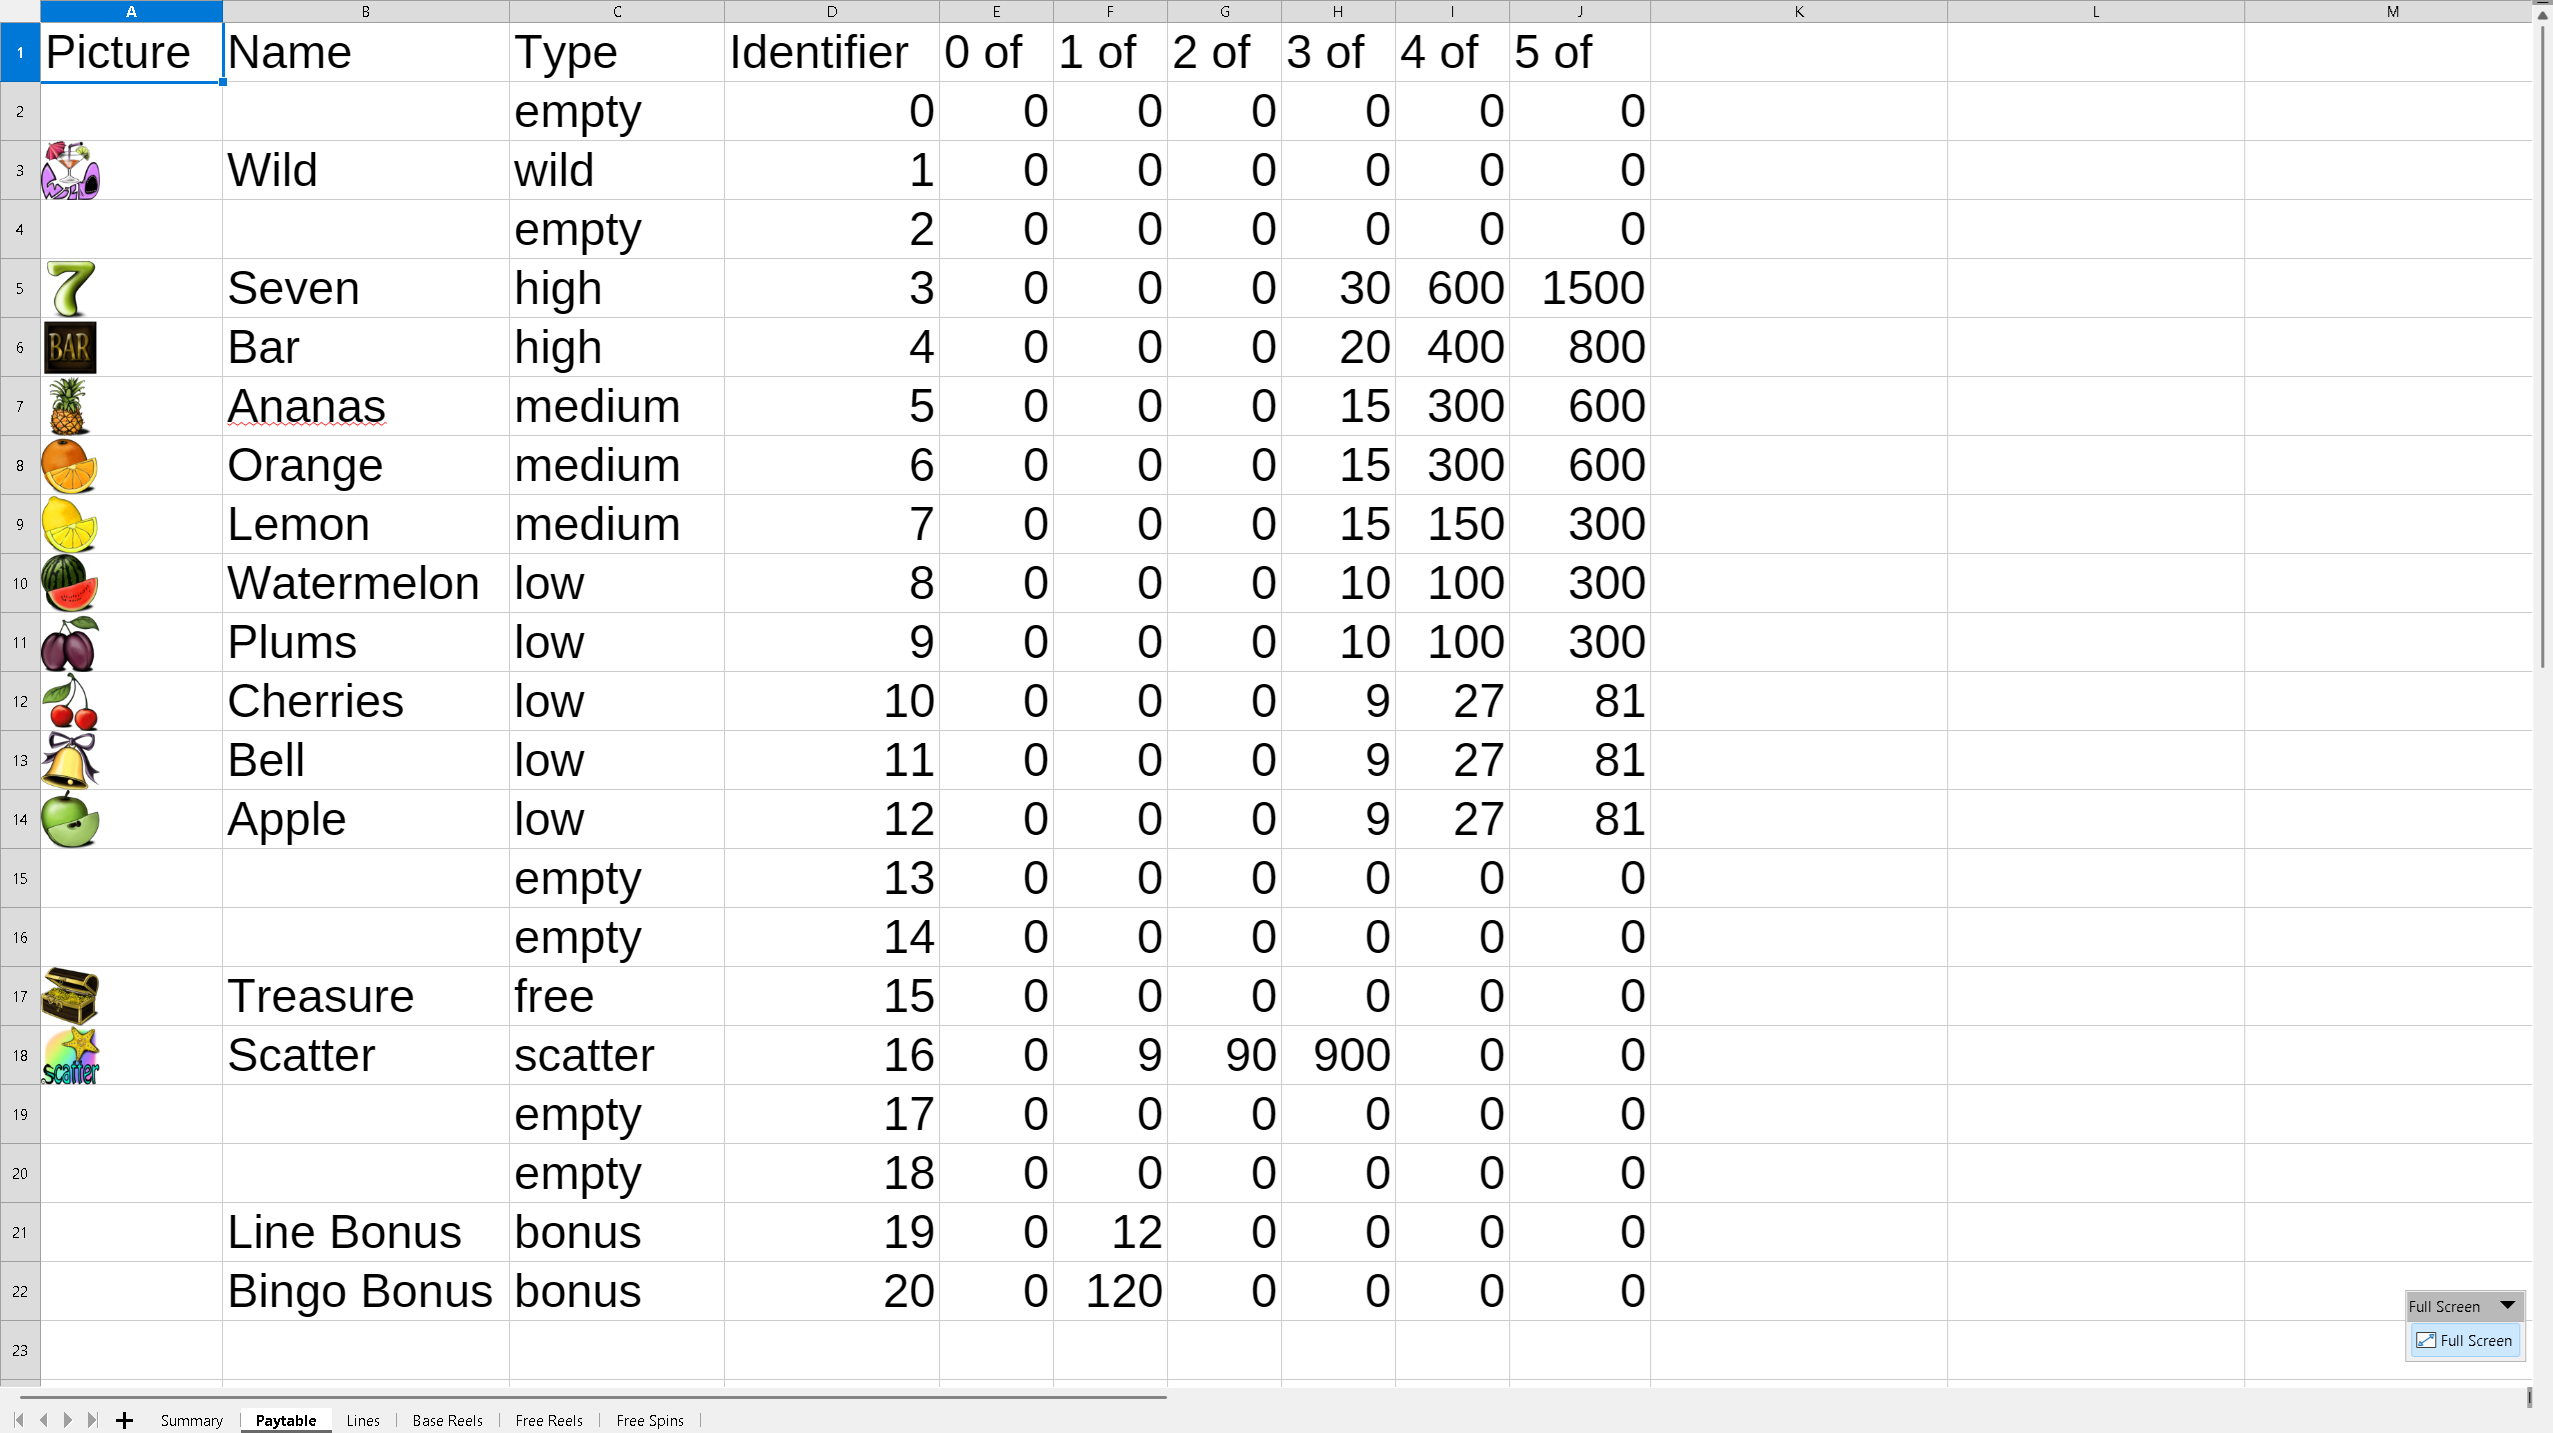
\includegraphics[width=\linewidth]{image029}
  \caption{Initial values for prizes in the paytable}
  \url{}
  \label{image029}
\end{figure}

The scatter, which triggers free spins, also does not reward a prize. It is easier to calculate the total win in each betting spin this way. It also keeps the RTP lower.

\chapter{Manual Reels Design}

The simulation is only a tool that helps game designers and mathematicians build the game model. There have been some attempts at automating game model building, but this work is still done manually. The free spins distribution was roughly designed. Because it is a book example, no special attention will be given to this. The free spins distribution could be used for fine adjustment if it were a real-life product.

\section*{Initial Reels}

Game reels are usually considered trade secrets of the game manufacturer. There is no problem with this information being revealed to players, but it keeps the game's mystery high, and gambling companies are hiding their reels very zealously. The art of slot game modeling comes in arranging the numbers on the reels.

The main goal in reel design is to achieve an RTP closer to the widely accepted levels (95.00\% for example). With the initialization of the reels, as shown in Listing \ref{listing031}, the achieved RTP is roughly in the range (96.17\%). The reason for this is how reels are initialized. The symbols are distributed relatively less often when winning combinations are high.

\begin{lstlisting}[language=bash, caption={Initial reels (histogram)}, label=listing031]
Base Game Symbol Frequencies:
0	0	0	0	0
1	1	1	1	1
0	0	0	0	0
1	1	1	1	1
2	2	2	2	2
3	3	3	3	3
4	4	4	4	4
3	5	5	5	7
7	5	5	5	3
5	5	8	2	5
7	7	4	10	7
15	4	9	9	10
5	14	9	9	10
0	0	0	0	0
0	0	0	0	0
0	1	1	1	0
0	1	1	1	0
0	0	0	0	0
0	0	0	0	0
0	0	0	0	0
0	0	0	0	0
0	0	0	0	0
0	0	0	0	0
0	0	0	0	0
0	0	0	0	0
0	0	0	0	0
0	0	0	0	0
0	0	0	0	0
0	0	0	0	0
0	0	0	0	0
0	0	0	0	0
0	0	0	0	0
0	0	0	0	0
0	0	0	0	0
0	0	0	0	0
0	0	0	0	0
0	0	0	0	0
0	0	0	0	0
0	0	0	0	0
0	0	0	0	0
0	0	0	0	0
0	0	0	0	0
0	0	0	0	0
0	0	0	0	0
0	0	0	0	0
0	0	0	0	0
0	0	0	0	0
0	0	0	0	0
0	0	0	0	0
0	0	0	0	0
0	0	0	0	0
0	0	0	0	0
0	0	0	0	0

53	53	53	53	53	418195493

Free Spins Symbol Frequencies:
0	0	0	0	0
0	1	1	1	0
0	0	0	0	0
1	1	1	1	1
2	2	2	2	2
3	3	3	3	3
4	4	4	4	4
5	5	5	5	5
5	5	5	5	5
5	5	5	5	5
7	7	7	7	7
10	9	9	9	10
11	10	10	10	11
0	0	0	0	0
0	0	0	0	0
0	0	0	0	0
0	1	1	1	0
0	0	0	0	0
0	0	0	0	0
0	0	0	0	0
0	0	0	0	0
0	0	0	0	0
0	0	0	0	0
0	0	0	0	0
0	0	0	0	0
0	0	0	0	0
0	0	0	0	0
0	0	0	0	0
0	0	0	0	0
0	0	0	0	0
0	0	0	0	0
0	0	0	0	0
0	0	0	0	0
0	0	0	0	0
0	0	0	0	0
0	0	0	0	0
0	0	0	0	0
0	0	0	0	0
0	0	0	0	0
0	0	0	0	0
0	0	0	0	0
0	0	0	0	0
0	0	0	0	0
0	0	0	0	0
0	0	0	0	0
0	0	0	0	0
0	0	0	0	0
0	0	0	0	0
0	0	0	0	0
0	0	0	0	0
0	0	0	0	0
0	0	0	0	0
0	0	0	0	0

53	53	53	53	53	418195493
\end{lstlisting}

There are different ways to form initial reels. The simplest method is to place symbols randomly. Random placement will lead to an almost equal distribution of each symbol. According to the paytable, it is not rational to expect an equal distribution of symbols. A more effective approach is subjective placement based on the intuition of each symbol's significance. In this initial version of the distribution, all symbols are grouped and sorted in each reel.

The base game reels and free spins reels are almost the same. Changes are made in both sets. The major difference is that free spins can not be retriggered from the free spins themselves. The free spins scatter is missing in the free spins reels.

After numerous manual adjustments, the triggering of free spins and scatter wins was significantly improved, and the total RTP reached 96.17\%. The problem in this stage is that symbols are still relatively sorted in the reels (Listing \ref{listing032}). After shuffling, the statistical parameters will not be the same.

\begin{lstlisting}[language=bash, caption={Initial reels (raw data)}, label=listing032]
Base Game Reels:
1	1	1	1	1
3	3	3	3	3
4	4	4	4	4
4	4	4	4	4
5	5	5	5	5
5	5	5	5	5
5	5	5	5	5
6	6	6	6	6
6	6	6	6	6
6	6	6	6	6
6	6	6	6	6
7	7	7	7	7
7	7	7	7	7
7	7	7	7	7
8	7	7	7	7
8	7	7	7	7
8	8	8	8	7
8	8	8	8	7
8	8	8	8	8
8	8	8	8	8
8	8	8	8	8
9	9	9	9	9
9	9	9	9	9
9	9	9	10	9
9	9	9	10	9
9	9	9	10	9
10	10	9	10	10
10	10	9	10	10
10	10	9	10	10
10	10	10	10	10
10	10	10	10	10
10	10	10	10	10
10	10	10	10	10
11	11	11	11	11
11	11	11	11	11
11	11	11	11	11
11	11	11	11	11
11	12	11	11	11
11	12	11	11	11
11	12	11	11	11
11	12	11	11	11
11	12	11	11	11
11	12	12	12	11
11	12	12	12	12
11	12	12	12	12
11	12	12	12	12
11	12	12	12	12
11	12	12	12	12
12	12	12	12	12
12	12	12	12	12
12	12	12	12	12
12	15	15	15	12
12	16	16	16	12

Free Spins Reels:
3	1	1	1	3
4	3	3	3	4
4	4	4	4	4
5	4	4	4	5
5	5	5	5	5
5	5	5	5	5
6	5	5	5	6
6	6	6	6	6
6	6	6	6	6
6	6	6	6	6
7	6	6	6	7
7	7	7	7	7
7	7	7	7	7
7	7	7	7	7
7	7	7	7	7
8	7	7	7	8
8	8	8	8	8
8	8	8	8	8
8	8	8	8	8
8	8	8	8	8
9	8	8	8	9
9	9	9	9	9
9	9	9	9	9
9	9	9	9	9
9	9	9	9	9
10	9	9	9	10
10	10	10	10	10
10	10	10	10	10
10	10	10	10	10
10	10	10	10	10
10	10	10	10	10
10	10	10	10	10
11	10	10	10	11
11	11	11	11	11
11	11	11	11	11
11	11	11	11	11
11	11	11	11	11
11	11	11	11	11
11	11	11	11	11
11	11	11	11	11
11	11	11	11	11
11	11	11	11	11
12	12	12	12	12
12	12	12	12	12
12	12	12	12	12
12	12	12	12	12
12	12	12	12	12
12	12	12	12	12
12	12	12	12	12
12	12	12	12	12
12	12	12	12	12
12	12	12	12	12
12	16	16	16	12
\end{lstlisting}

\section*{Shuffling and Final Adjustment}

Partially sorted reels are now handy in a real game. Because of this, each reel should be shuffled, and some rules should be observed. Shuffling can be done in many different ways, including manual inclusion. Developed reels are shuffled by putting reels in LibreOffice Calc as columns and adding an extra column with randomly generated numbers. Consecutive sortings are done by giving the sorting order from the randomly generated numbers column. It is not industry-reliable shuffling, but it is acceptable as a quick example.

\begin{lstlisting}[language=bash, caption={Shuffled reels (raw data)}, label=listing033]
Base Game Reels:
7	10	12	7	9
3	5	12	5	9
11	16	5	5	7
7	8	11	16	4
11	10	9	6	6
11	10	11	5	12
6	12	4	6	10
10	12	6	11	12
10	12	7	7	6
5	10	6	12	9
12	9	9	10	10
8	11	10	12	10
4	8	11	12	9
10	12	9	1	10
10	12	7	4	10
11	7	7	6	11
11	8	11	11	4
12	12	9	8	12
8	10	7	12	12
8	6	11	10	12
12	7	7	10	9
5	12	12	6	1
11	12	3	8	6
11	7	11	12	8
9	6	12	9	6
6	4	6	8	11
8	12	8	10	10
4	10	4	9	7
9	15	8	12	11
9	12	12	12	11
11	11	8	11	5
11	9	11	4	11
11	7	11	10	12
9	12	9	11	10
8	4	12	10	7
7	8	5	11	11
6	9	9	8	12
11	11	6	11	5
11	6	11	7	7
12	3	9	15	3
10	6	8	11	11
10	5	12	7	7
12	1	1	7	7
10	12	12	12	12
1	11	10	12	12
11	9	12	10	11
8	8	8	3	5
9	5	5	8	7
6	10	10	11	11
11	12	15	10	8
11	9	16	11	11
8	12	10	10	12
5	7	9	10	8

Free Spins Reels:
7	11	8	11	9
8	10	7	12	12
6	12	12	10	9
9	8	9	12	12
10	12	9	12	5
6	10	4	9	8
11	11	1	9	7
12	11	11	7	11
11	11	5	6	9
4	8	10	7	8
12	8	9	12	12
12	12	6	12	11
9	11	10	9	10
10	12	12	10	12
5	10	12	1	9
10	7	3	6	7
10	12	8	12	4
10	4	4	11	7
10	11	6	10	11
12	9	7	9	12
8	6	6	3	10
4	4	10	4	10
9	5	12	6	9
11	12	16	10	12
7	12	10	8	11
11	5	11	8	12
12	9	9	8	6
11	16	7	10	11
12	7	10	11	8
6	11	11	8	10
11	6	6	12	8
8	10	7	10	5
9	3	5	12	12
12	5	12	7	12
7	10	12	11	7
12	9	11	11	12
3	7	12	4	7
12	12	12	12	6
11	12	11	11	11
9	11	10	5	12
7	10	7	11	6
8	7	11	10	10
11	6	8	11	8
5	12	11	16	11
12	9	8	12	4
11	9	8	5	11
8	6	11	11	10
5	1	12	7	11
10	8	5	6	6
11	8	9	5	5
7	11	11	7	11
6	10	10	8	3
12	7	12	9	10
\end{lstlisting}

After shuffling the symbols on the reels, the RTP decreases slightly to 96.06\% (Listing \ref{listing033}).

\chapter{Volatility Analysis}

Slot game volatility is a key aspect of the game's mathematical design. Generally, game volatility is rated from 1 (low) to 5 (high) stars in published games. Low volatility is typically associated with games offering small prizes, but often given, while high volatility is associated with games offering big prizes, but given rarely. Volatility is essential for the markets in which the game will be operated. Markets with risk-taking players are proper for high-volatility games. Markets with no risk-taking players are appropriate for low-volatility games. Here comes the question of how volatility is to be estimated.

\section*{Low and High Volatility Reels}

An engineering approach to estimating a game's volatility is to arrange high- and low-volatility reels. By analyzing RTP dynamics across designed game reels and high/low-volatility reels, the game can be categorized under the 5-star scheme.

Free spins can be skipped for a low-volatility version of the designed math, and only a low-paying symbol can form winning combinations. Free spins will not be awarded if the free spins scatter symbol is not presented on the reels (Listing \ref{listing034}).

\begin{lstlisting}[language=bash, caption={Low volatile reels (raw data)}, label=listing034]
Base Game Reels:
12	11	10	9	8
12	11	10	9	8
12	11	10	9	8
12	12	10	9	8
12	11	10	9	8
12	11	10	9	8
12	12	10	9	8
12	11	10	9	8
12	11	10	9	8
12	11	12	9	8
12	11	10	9	8
12	11	12	9	8
12	11	10	9	8
12	11	10	9	8
12	11	12	9	8
12	12	10	9	8
12	12	10	9	8
12	11	10	9	8
12	11	10	9	8
12	11	10	9	8
12	12	10	9	8
12	11	12	9	8
12	11	10	9	8
12	11	10	9	8
12	12	12	9	8
12	11	10	9	8
12	12	10	9	8
12	12	10	9	8
12	11	10	9	8
12	11	10	9	8
12	11	10	9	8
12	11	10	9	8
12	11	12	9	8
12	11	12	9	8
12	11	10	9	8
12	11	12	9	8
12	11	10	9	8
12	12	10	9	8
12	11	10	9	8
12	11	10	9	8
12	12	12	9	8
12	11	10	9	8
12	11	12	9	8
12	11	12	9	8
12	12	10	9	8
12	12	10	9	8
12	11	10	9	8
12	11	10	9	8
12	11	10	9	8
12	11	10	9	8
12	11	10	9	8
12	11	10	9	8
12	11	12	9	8
\end{lstlisting}

Reels are used in 30 independent game simulations (Figure \ref{image021}). The number 30 is taken empirically from the statistics and the theory of the Normal Probability Distribution. As it is seen, there is a funnel representing the RTP convergence. Measurements are done in increments of 10 thousand base game spins for a total of 10 million spins.

\begin{figure}[htbp]
  \centering
  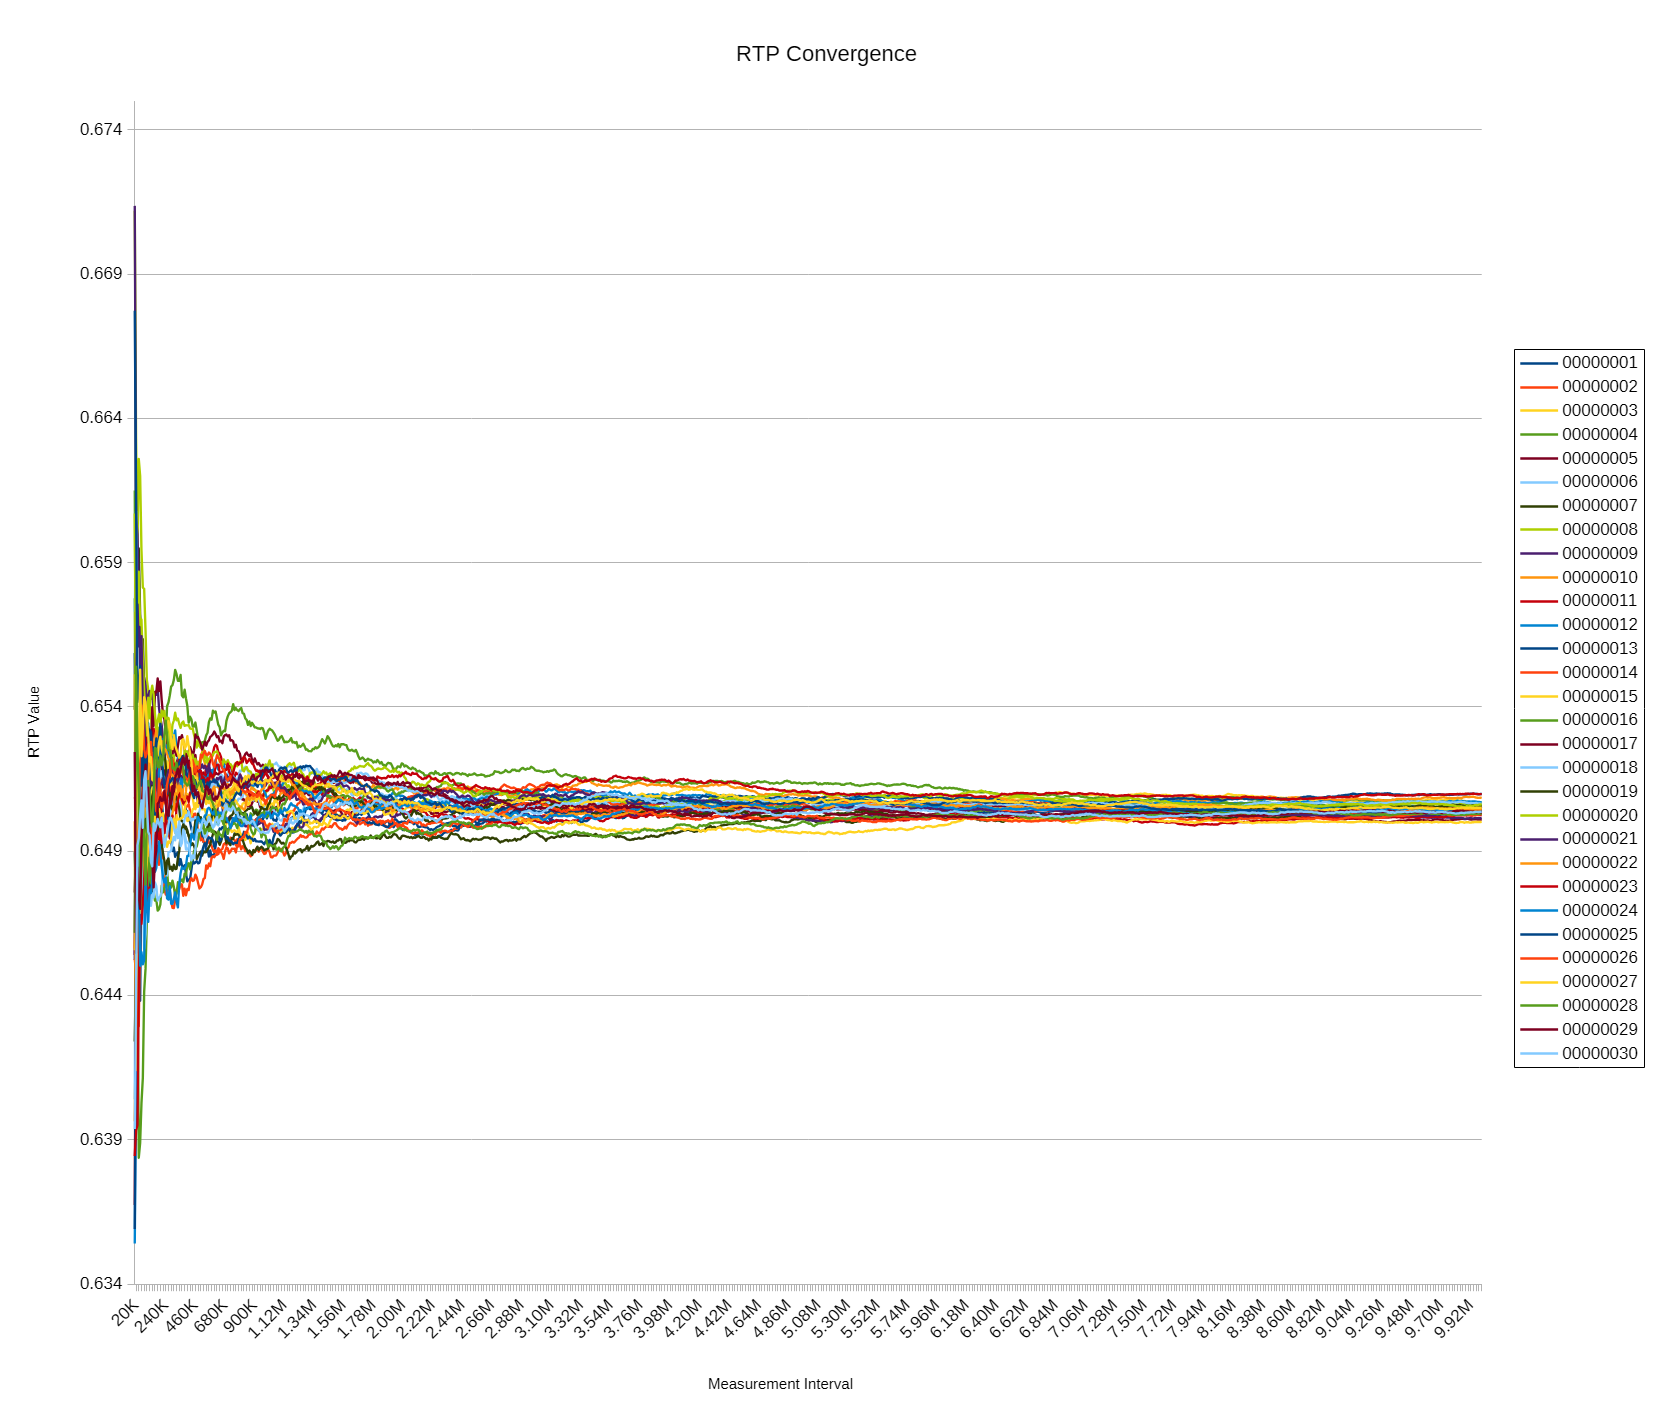
\includegraphics[width=\linewidth]{image021}
  \caption{Low-volatile RTP convergence}
  \url{}
  \label{image021}
\end{figure}

High-volatility reels can be designed by skipping the free spins and offering only prizes from the highest-paying symbol (Listing \ref{listing035}). According to the paytable used, such a symbol is the Seven.

\begin{lstlisting}[language=bash, caption={Highly volatile reels (raw data)}, label=listing035]
Base Game Reels:
4	5	3	3	3
4	5	6	3	3
4	5	3	3	3
4	5	3	3	3
4	5	3	3	3
4	5	3	3	3
4	5	3	3	3
4	5	3	3	3
4	5	3	3	3
4	5	3	3	3
4	5	3	3	3
4	5	3	3	3
4	5	3	3	3
4	5	3	3	3
4	5	3	3	3
4	5	6	3	3
4	5	3	3	3
4	5	6	3	3
4	5	6	3	3
4	5	3	3	3
4	5	3	3	3
4	5	3	3	3
4	5	3	3	3
4	5	6	3	3
4	5	3	3	3
4	5	3	3	3
4	5	3	3	3
4	5	3	3	3
4	5	3	3	3
4	5	3	3	3
4	5	3	3	3
4	5	3	3	3
4	5	3	3	3
4	5	3	3	3
4	5	3	3	3
4	5	6	3	3
4	5	3	3	3
4	5	6	3	3
4	5	3	3	3
4	5	3	3	3
4	5	3	3	3
4	5	3	3	3
4	5	3	3	3
4	5	3	3	3
3	5	3	3	3
4	5	3	3	3
4	5	3	3	3
4	5	3	3	3
4	5	3	3	3
4	3	3	3	3
4	5	3	3	3
4	5	3	3	3
4	5	3	3	3
\end{lstlisting}

Once again, 30 independent spins are done (Figure \ref{image018}). The funnel is much wider because the prizes are more distant from the central tendency.

\begin{figure}[htbp]
  \centering
  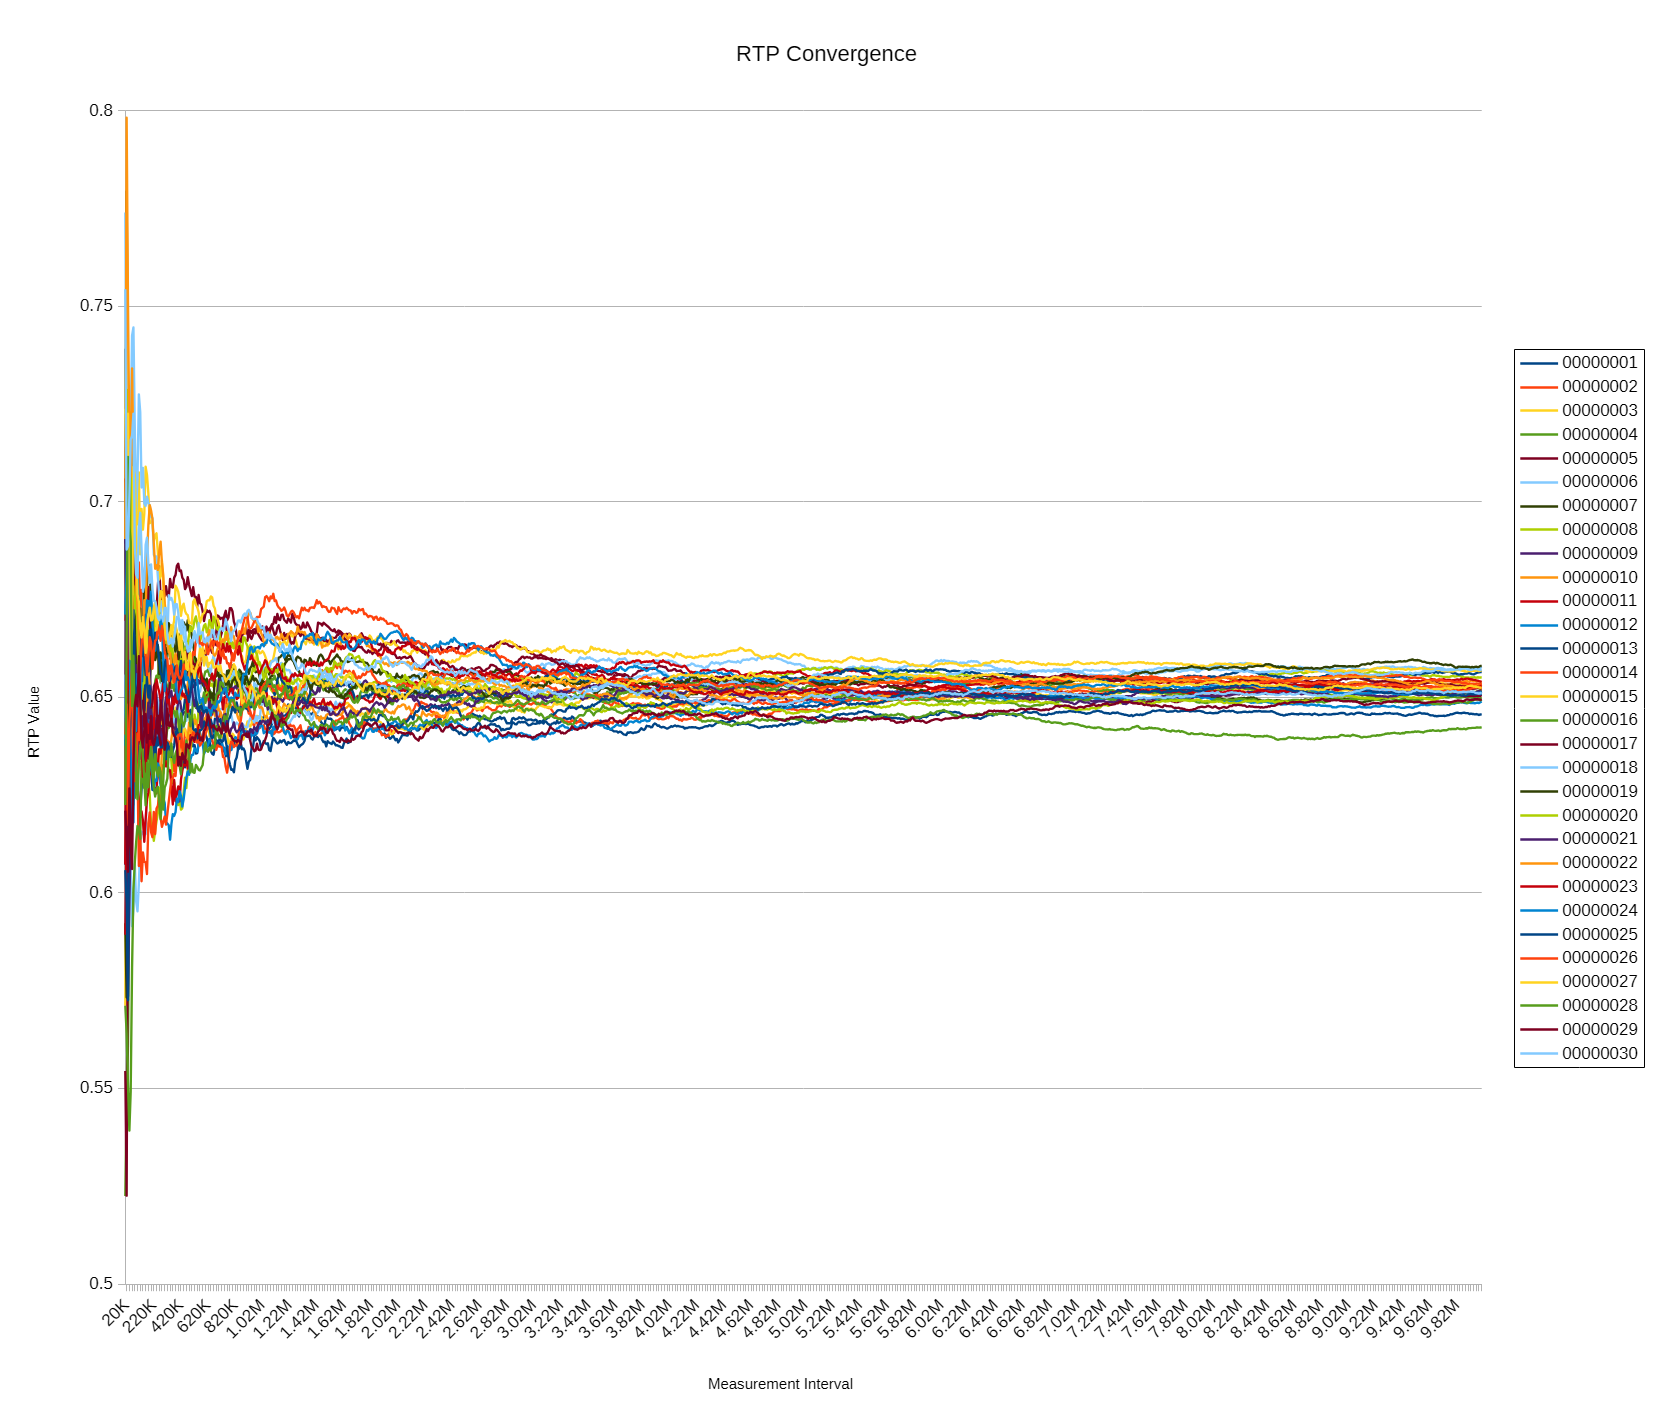
\includegraphics[width=\linewidth]{image018}
  \caption{High-volatility RTP convergence}
  \url{}
  \label{image018}
\end{figure}

An additional 30 independent runs are simulated using the original reels (Figure \ref{image020}).

\begin{figure}[htbp]
  \centering
  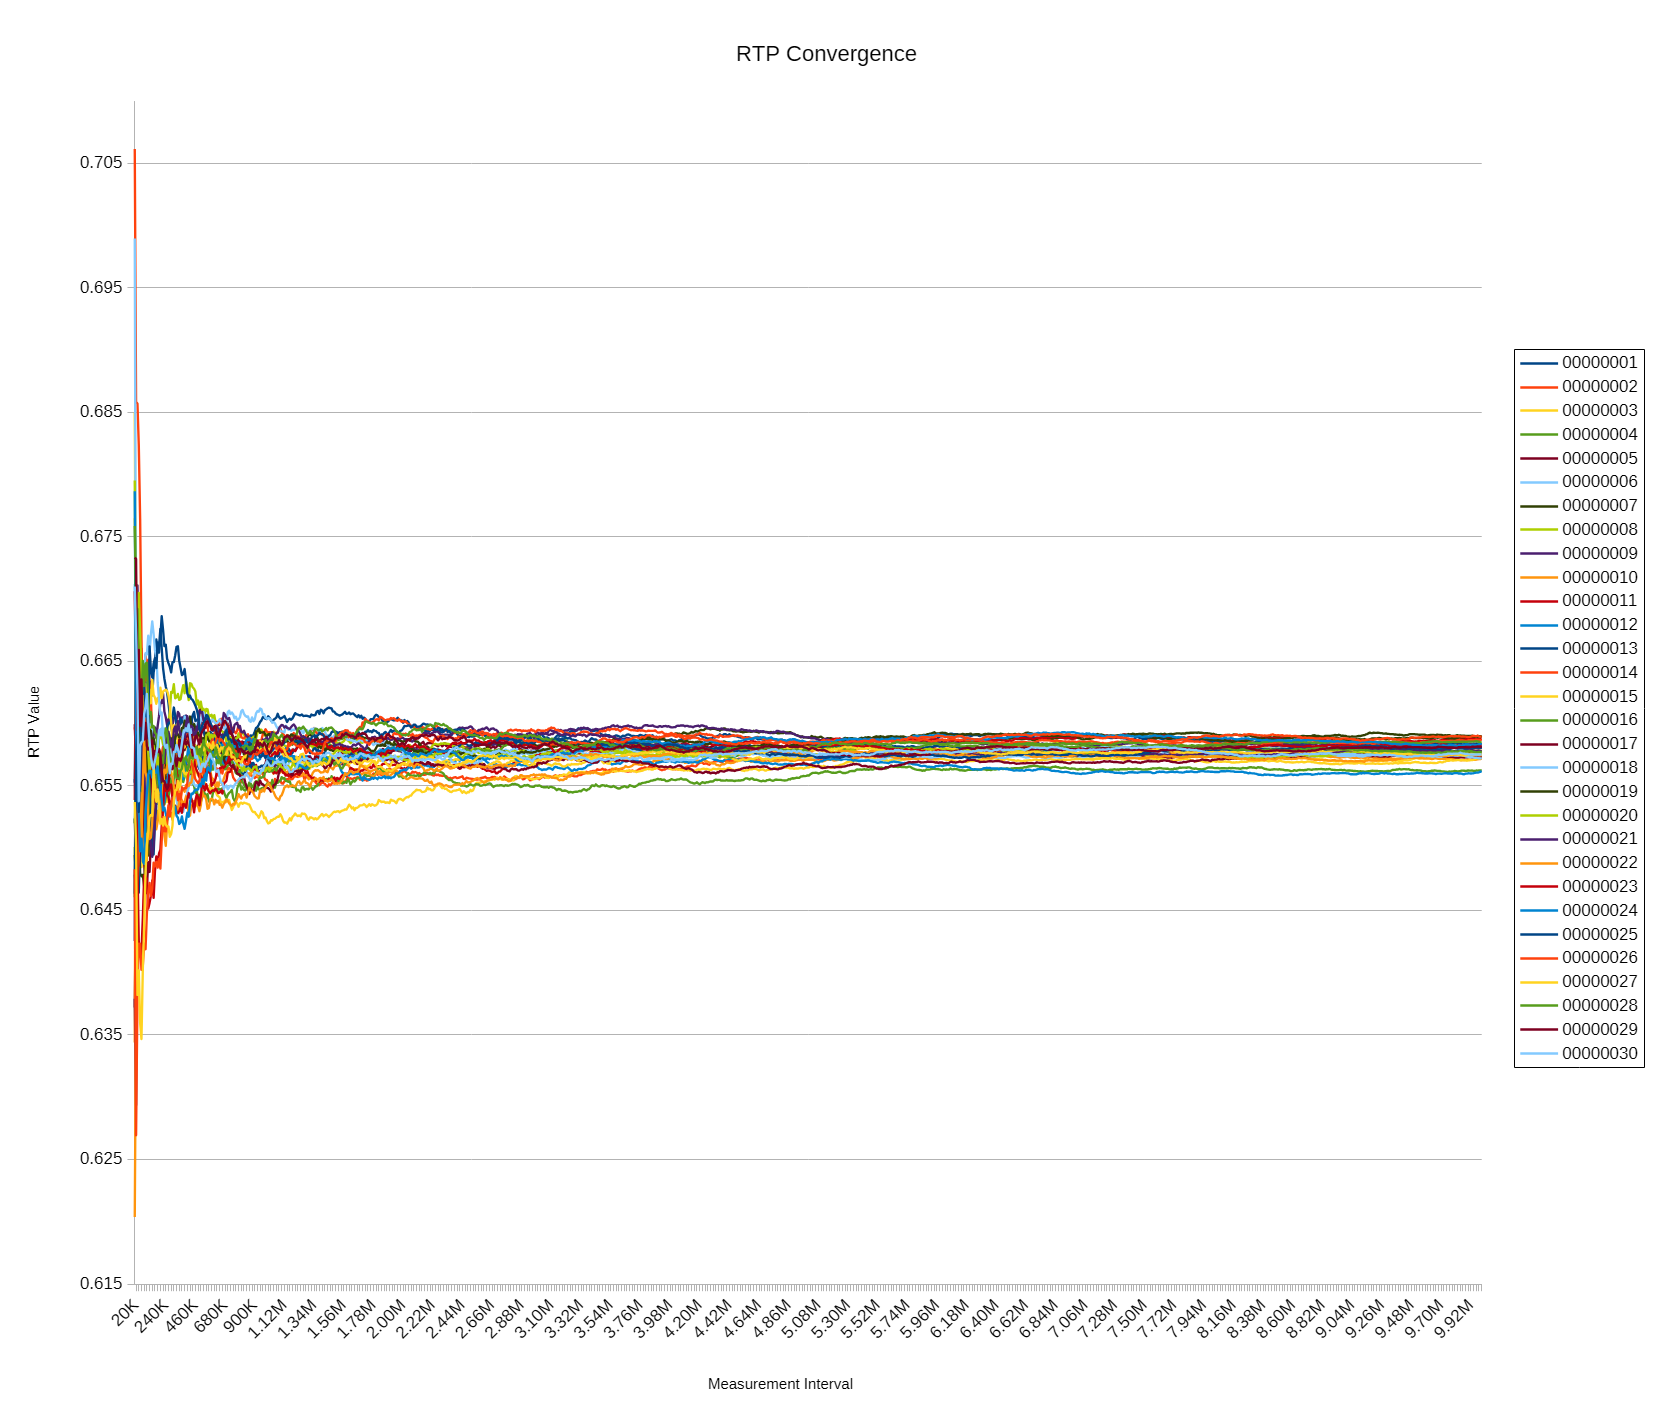
\includegraphics[width=\linewidth]{image020}
  \caption{Designed reels RTP convergence}
  \url{}
  \label{image020}
\end{figure}

\section*{Comparison of Volatilities}

A comparison of volatilities can estimate the volatility achieved by designed reels. Such comparisons can be made numerically, but only visual analysis is given in the current situation (Figure \ref{image019}).

\begin{figure}[htbp]
  \centering
  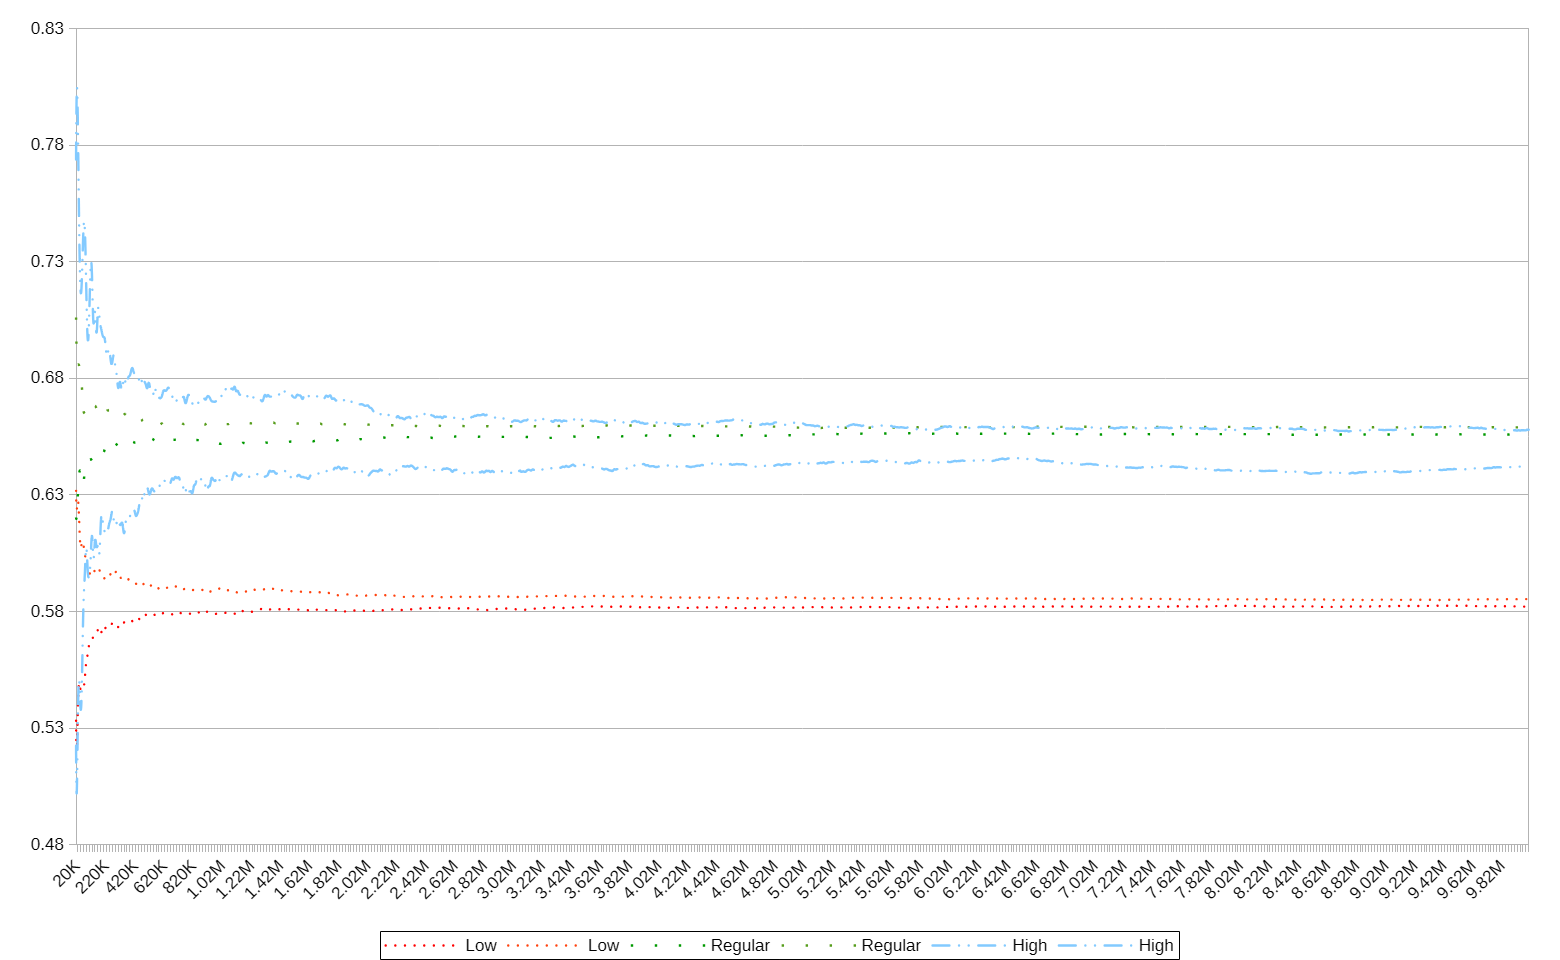
\includegraphics[width=\linewidth]{image019}
  \caption{Volatility funnels}
  \url{}
  \label{image019}
\end{figure}

The convergence funnels are in different colors and dot patterns. The blue line (marked as High in the legend) shows the highly volatile reels, the red line (marked as Low in the legend) shows the low volatile reels, and the green line (marked as Regular in the legend) shows the designed reels. The central tendency differs slightly on the graph. The reason is that the target RTP was not followed strictly. The main accent was RTP deviation. By examining the graph, it is evident that designed reels are suitable for relatively low volatility. Volatility can be adjusted by redesigning the reels further, which involves raising the number of big prizes and lowering the number of small prizes. Another way to adjust for volatility is by regulating the scatter win frequency.

\chapter{Analytical RTP}



\chapter*{Final Remarks}

This book introduces the practical aspects of mathematical modeling in slot machine games. For the base of the modeling, a Monte Carlo simulation is used. Even though a theoretical approach can be applied, when the games are very complicated, the Monte Carlo simulation remains the only option. The book shows only the standard steps for creating a mathematical model. There are many other factors to consider in actual industrial production. Game studio managers may require many parameters to have values within particular ranges, except for the RTP. It is up to the reader to extend the knowledge acquired from this book.

The author would like to thank all readers for taking the time to read this book. The reader is encouraged to develop his/her knowledge and skills in this field and to share discoveries with the author if they wish.

% --- BACK MATTER ---
\backmatter

\chapter*{About the Author}
Todor has a Ph.D. in Informatics and Computer Sciences. He also has an MSc in Internet Software Technologies, an MSc in Data Analysis with Specialized Software, a BSc in Computer Systems and Technologies, and a BSc in Informatics. Currently, he is an associate at the Institute of Information and Communication Technologies, part of the Bulgarian Academy of Sciences. He has taught at some of the most highly rated Bulgarian universities, like New Bulgarian University, Technical University of Sofia, and Sofia University. He has written books about software development and applied statistics. Todor has many scientific publications. What he likes the most are good challenges. In his leisure time, he enjoys traveling and going out with friends. He is unmarried and has one child.

\begin{thebibliography}{99}
\bibitem{Parvanov-2021} Parvanov, D., Mateeva, G., Balabanov, T.: Classification of Images for Reverse Engineering of Slot Machines, Abstracts of the 16th Annual Meeting of the Bulgarian Section of SIAM, Fastumprint, 36-37, 2021, ISSN 1313-3357
\bibitem{Balabanov-2021a} Balabanov, T.: Volatility Index Estimation by Reverse Engineering, Proceedings of the International Scientific Conference UNITECH, vol. 1, 229-234, 2021, ISSN 1313-230X
\bibitem{Balabanov-2021b} Balabanov, T.: Estimation of Volatility based on the Estimation of Segmentation, Problems of Engineering Cybernetics and Robotics, vol. 77, 3-10, 2021, ISSN 2738-7356
\bibitem{Petrov-2020} Petrov, P., Kostadinov, G., Zhivkov, P., Velichkova, V., Balabanov, T.: Approximate Sequencing of Virtual Reels with Genetic Algorithms, Proceedings of the 23rd International Conference on Distributed Computer and Communication Networks: Control, Computation, Communications, 507-514, 2020, ISBN 978-5-91450-248-2
\bibitem{Tomov-2017a} Tomov, P., Zankinski. I., Balabanov, T.: Slot Machine Reels Reconstruction with Genetic Algorithms, Abstracts of the 12th Annual Meeting of the Bulgarian Section of SIAM, Fastumprint, 102-103, 2017, ISSN 1313-3357
\bibitem{Tomov-2017b} Tomov, P., Zankinski. I.., Balabanov, T.: Slot Machine Reels Reconstruction with Monte-Carlo Search, Proceedings of the International Scientific Conference UNITECH, vol. 2, 384-387, 2017, ISSN 1313-230X
\bibitem{Balabanov-2015} Balabanov, T., Zankinski. I.., Shumanov, B.: Slot Machine RTP Optimization and Symbols Wins Equalization with Discrete Differential Evolution, Proceedings of the International Conference on Large-Scale Scientific Computing, vol. 9374, 210–217, 2015, ISBN 978-3-319-26519-3
\bibitem{Balabanov-2014} Balabanov, T., Zankinski. I.., Shumanov, B.: Slot Machines RTP Optimization with Genetic Algorithms, Proceedings of the International Conference on Numerical Methods and Applications, vol. 8962, 55-61, 2014, ISBN 978-3-319-15584-5
\bibitem{Keremedchiev-2017} Keremedchiev, D., Tomov, P., Barova, M.: Slot Machine Base Game Evolutionary RTP Optimization, Proceedings of the International Conference on Numerical Analysis and Its Applications, vol. 10187, 406-413, 2017, ISBN 978-3-319-57098-3
\bibitem{Kamana-2021a} Kamana, P.A., Sifaleras, A., Samaras, N.: Slot Machine RTP Optimization Using Variable Neighborhood Search, Mathematical Problems in Engineering, 8784065, 2021, ISSN 1024-123X
\bibitem{Kamana-2021b} Kamana, P.A.: Design and Analysis of Slot Machine Games and RTP Optimization Using Variable Neighborhood Search (VNS), Master of Science Thesis, Thessaloniki, 2021
\end{thebibliography}

\end{document}
